% Options for packages loaded elsewhere
\PassOptionsToPackage{unicode}{hyperref}
\PassOptionsToPackage{hyphens}{url}
%
\documentclass[
]{book}
\usepackage{amsmath,amssymb}
\usepackage{lmodern}
\usepackage{iftex}
\ifPDFTeX
  \usepackage[T1]{fontenc}
  \usepackage[utf8]{inputenc}
  \usepackage{textcomp} % provide euro and other symbols
\else % if luatex or xetex
  \usepackage{unicode-math}
  \defaultfontfeatures{Scale=MatchLowercase}
  \defaultfontfeatures[\rmfamily]{Ligatures=TeX,Scale=1}
\fi
% Use upquote if available, for straight quotes in verbatim environments
\IfFileExists{upquote.sty}{\usepackage{upquote}}{}
\IfFileExists{microtype.sty}{% use microtype if available
  \usepackage[]{microtype}
  \UseMicrotypeSet[protrusion]{basicmath} % disable protrusion for tt fonts
}{}
\makeatletter
\@ifundefined{KOMAClassName}{% if non-KOMA class
  \IfFileExists{parskip.sty}{%
    \usepackage{parskip}
  }{% else
    \setlength{\parindent}{0pt}
    \setlength{\parskip}{6pt plus 2pt minus 1pt}}
}{% if KOMA class
  \KOMAoptions{parskip=half}}
\makeatother
\usepackage{xcolor}
\IfFileExists{xurl.sty}{\usepackage{xurl}}{} % add URL line breaks if available
\IfFileExists{bookmark.sty}{\usepackage{bookmark}}{\usepackage{hyperref}}
\hypersetup{
  pdftitle={Lecture notes for "Introduction to Stochastic Processes"},
  pdfauthor={Gordan Zitkovic},
  hidelinks,
  pdfcreator={LaTeX via pandoc}}
\urlstyle{same} % disable monospaced font for URLs
\usepackage{color}
\usepackage{fancyvrb}
\newcommand{\VerbBar}{|}
\newcommand{\VERB}{\Verb[commandchars=\\\{\}]}
\DefineVerbatimEnvironment{Highlighting}{Verbatim}{commandchars=\\\{\}}
% Add ',fontsize=\small' for more characters per line
\usepackage{framed}
\definecolor{shadecolor}{RGB}{248,248,248}
\newenvironment{Shaded}{\begin{snugshade}}{\end{snugshade}}
\newcommand{\AlertTok}[1]{\textcolor[rgb]{0.94,0.16,0.16}{#1}}
\newcommand{\AnnotationTok}[1]{\textcolor[rgb]{0.56,0.35,0.01}{\textbf{\textit{#1}}}}
\newcommand{\AttributeTok}[1]{\textcolor[rgb]{0.77,0.63,0.00}{#1}}
\newcommand{\BaseNTok}[1]{\textcolor[rgb]{0.00,0.00,0.81}{#1}}
\newcommand{\BuiltInTok}[1]{#1}
\newcommand{\CharTok}[1]{\textcolor[rgb]{0.31,0.60,0.02}{#1}}
\newcommand{\CommentTok}[1]{\textcolor[rgb]{0.56,0.35,0.01}{\textit{#1}}}
\newcommand{\CommentVarTok}[1]{\textcolor[rgb]{0.56,0.35,0.01}{\textbf{\textit{#1}}}}
\newcommand{\ConstantTok}[1]{\textcolor[rgb]{0.00,0.00,0.00}{#1}}
\newcommand{\ControlFlowTok}[1]{\textcolor[rgb]{0.13,0.29,0.53}{\textbf{#1}}}
\newcommand{\DataTypeTok}[1]{\textcolor[rgb]{0.13,0.29,0.53}{#1}}
\newcommand{\DecValTok}[1]{\textcolor[rgb]{0.00,0.00,0.81}{#1}}
\newcommand{\DocumentationTok}[1]{\textcolor[rgb]{0.56,0.35,0.01}{\textbf{\textit{#1}}}}
\newcommand{\ErrorTok}[1]{\textcolor[rgb]{0.64,0.00,0.00}{\textbf{#1}}}
\newcommand{\ExtensionTok}[1]{#1}
\newcommand{\FloatTok}[1]{\textcolor[rgb]{0.00,0.00,0.81}{#1}}
\newcommand{\FunctionTok}[1]{\textcolor[rgb]{0.00,0.00,0.00}{#1}}
\newcommand{\ImportTok}[1]{#1}
\newcommand{\InformationTok}[1]{\textcolor[rgb]{0.56,0.35,0.01}{\textbf{\textit{#1}}}}
\newcommand{\KeywordTok}[1]{\textcolor[rgb]{0.13,0.29,0.53}{\textbf{#1}}}
\newcommand{\NormalTok}[1]{#1}
\newcommand{\OperatorTok}[1]{\textcolor[rgb]{0.81,0.36,0.00}{\textbf{#1}}}
\newcommand{\OtherTok}[1]{\textcolor[rgb]{0.56,0.35,0.01}{#1}}
\newcommand{\PreprocessorTok}[1]{\textcolor[rgb]{0.56,0.35,0.01}{\textit{#1}}}
\newcommand{\RegionMarkerTok}[1]{#1}
\newcommand{\SpecialCharTok}[1]{\textcolor[rgb]{0.00,0.00,0.00}{#1}}
\newcommand{\SpecialStringTok}[1]{\textcolor[rgb]{0.31,0.60,0.02}{#1}}
\newcommand{\StringTok}[1]{\textcolor[rgb]{0.31,0.60,0.02}{#1}}
\newcommand{\VariableTok}[1]{\textcolor[rgb]{0.00,0.00,0.00}{#1}}
\newcommand{\VerbatimStringTok}[1]{\textcolor[rgb]{0.31,0.60,0.02}{#1}}
\newcommand{\WarningTok}[1]{\textcolor[rgb]{0.56,0.35,0.01}{\textbf{\textit{#1}}}}
\usepackage{longtable,booktabs,array}
\usepackage{calc} % for calculating minipage widths
% Correct order of tables after \paragraph or \subparagraph
\usepackage{etoolbox}
\makeatletter
\patchcmd\longtable{\par}{\if@noskipsec\mbox{}\fi\par}{}{}
\makeatother
% Allow footnotes in longtable head/foot
\IfFileExists{footnotehyper.sty}{\usepackage{footnotehyper}}{\usepackage{footnote}}
\makesavenoteenv{longtable}
\usepackage{graphicx}
\makeatletter
\def\maxwidth{\ifdim\Gin@nat@width>\linewidth\linewidth\else\Gin@nat@width\fi}
\def\maxheight{\ifdim\Gin@nat@height>\textheight\textheight\else\Gin@nat@height\fi}
\makeatother
% Scale images if necessary, so that they will not overflow the page
% margins by default, and it is still possible to overwrite the defaults
% using explicit options in \includegraphics[width, height, ...]{}
\setkeys{Gin}{width=\maxwidth,height=\maxheight,keepaspectratio}
% Set default figure placement to htbp
\makeatletter
\def\fps@figure{htbp}
\makeatother
\setlength{\emergencystretch}{3em} % prevent overfull lines
\providecommand{\tightlist}{%
  \setlength{\itemsep}{0pt}\setlength{\parskip}{0pt}}
\setcounter{secnumdepth}{5}
\usepackage{booktabs}
\usepackage{longtable}
\usepackage{array}
\usepackage{multirow}
\usepackage{wrapfig}
\usepackage{float}
\usepackage{colortbl}
\usepackage{pdflscape}
\usepackage{tabu}
\usepackage{threeparttable}
\usepackage{threeparttablex}
\usepackage[normalem]{ulem}
\usepackage{makecell}
\usepackage{xcolor}
\ifLuaTeX
  \usepackage{selnolig}  % disable illegal ligatures
\fi

\title{Lecture notes for "Introduction to Stochastic Processes"}
\author{Gordan Zitkovic}
\date{last updated - 2021-12-11}

\usepackage{amsthm}
\newtheorem{theorem}{Theorem}[chapter]
\newtheorem{lemma}{Lemma}[chapter]
\newtheorem{corollary}{Corollary}[chapter]
\newtheorem{proposition}{Proposition}[chapter]
\newtheorem{conjecture}{Conjecture}[chapter]
\theoremstyle{definition}
\newtheorem{definition}{Definition}[chapter]
\theoremstyle{definition}
\newtheorem{example}{Example}[chapter]
\theoremstyle{definition}
\newtheorem{exercise}{Problem}[chapter]
\theoremstyle{definition}
\newtheorem{hypothesis}{Hypothesis}[chapter]
\theoremstyle{remark}
\newtheorem*{remark}{Remark}
\newtheorem*{solution}{Solution}
\begin{document}
\maketitle

{
\setcounter{tocdepth}{1}
\tableofcontents
}
\hypertarget{preface}{%
\chapter*{Preface}\label{preface}}
\addcontentsline{toc}{chapter}{Preface}

This is an ever-evolving set of lecture notes for \textbf{Introduction to Stochastic Processes (M362M)}. It should start with me explaining what stochastic processes are. Instead, here is a list of several questions you will be able to give answers to when you complete this course.

\textbf{Question 1} In a simplistic model, the price of a share of a stock goes either up or down by \(\$1\) each day, with probability \(1/2\). You own a single share whose value today is \(\$100\), so that its tomorrow's price will be \(\$101\) or \(\$99\) with probability \(1/2\), etc. Your strategy is to hold onto your share until one of the following two things happen: you go bankrupt (the stock price hits \(0\)), or you make a \(\$50\) dollar profit (the stock price hits \(\$150\).)

\begin{enumerate}
\def\labelenumi{\arabic{enumi}.}
\tightlist
\item
  How likely is it that you will make a profit before you go bankrupt?
\item
  How long will it take?
\item
  Is it possible that it takes forever, i.e., that the stock price hovers between \(\$1\) and \(\$149\) forever?
\end{enumerate}

\textbf{Question 2.} A person carrying a certain disease infects a random number of people in a week, and then stops being infectious. Each of the infected people transmits the disease in the same way, etc. Suppose that the number of people each (infectious) individual infects is either \(0\), \(1\) or \(2\) or \(3\), each with probability \(1/4\) and that different infectious individuals may infect different number of people and behave independently of each other.

\begin{enumerate}
\def\labelenumi{\arabic{enumi}.}
\tightlist
\item
  What is the probability that the disease will ever be eradicated?
\item
  What is the probability that every single individual in the population of \(328,000,000\) will eventually be infected?
\end{enumerate}

\textbf{Question 3.} In a game of tennis, Player \(1\) wins against Player \(2\) in each rally (the smallest chunk of the match that leads to point, i.e., to a score change from \(15-30\) to \(30-30\), for example) with probability \(p\).
What is the probability that Player \(1\) wins

\begin{enumerate}
\def\labelenumi{\arabic{enumi}.}
\tightlist
\item
  a game (the chunk of the match that leads to a score change such as \(5-3\) to \(6-3\) within a set)?
\item
  a set? the entire match?
\item
  Is the game of tennis set up in such a way that is \emph{amplifies} or \emph{reduces} the difference in skill between players?
\end{enumerate}

\begin{center}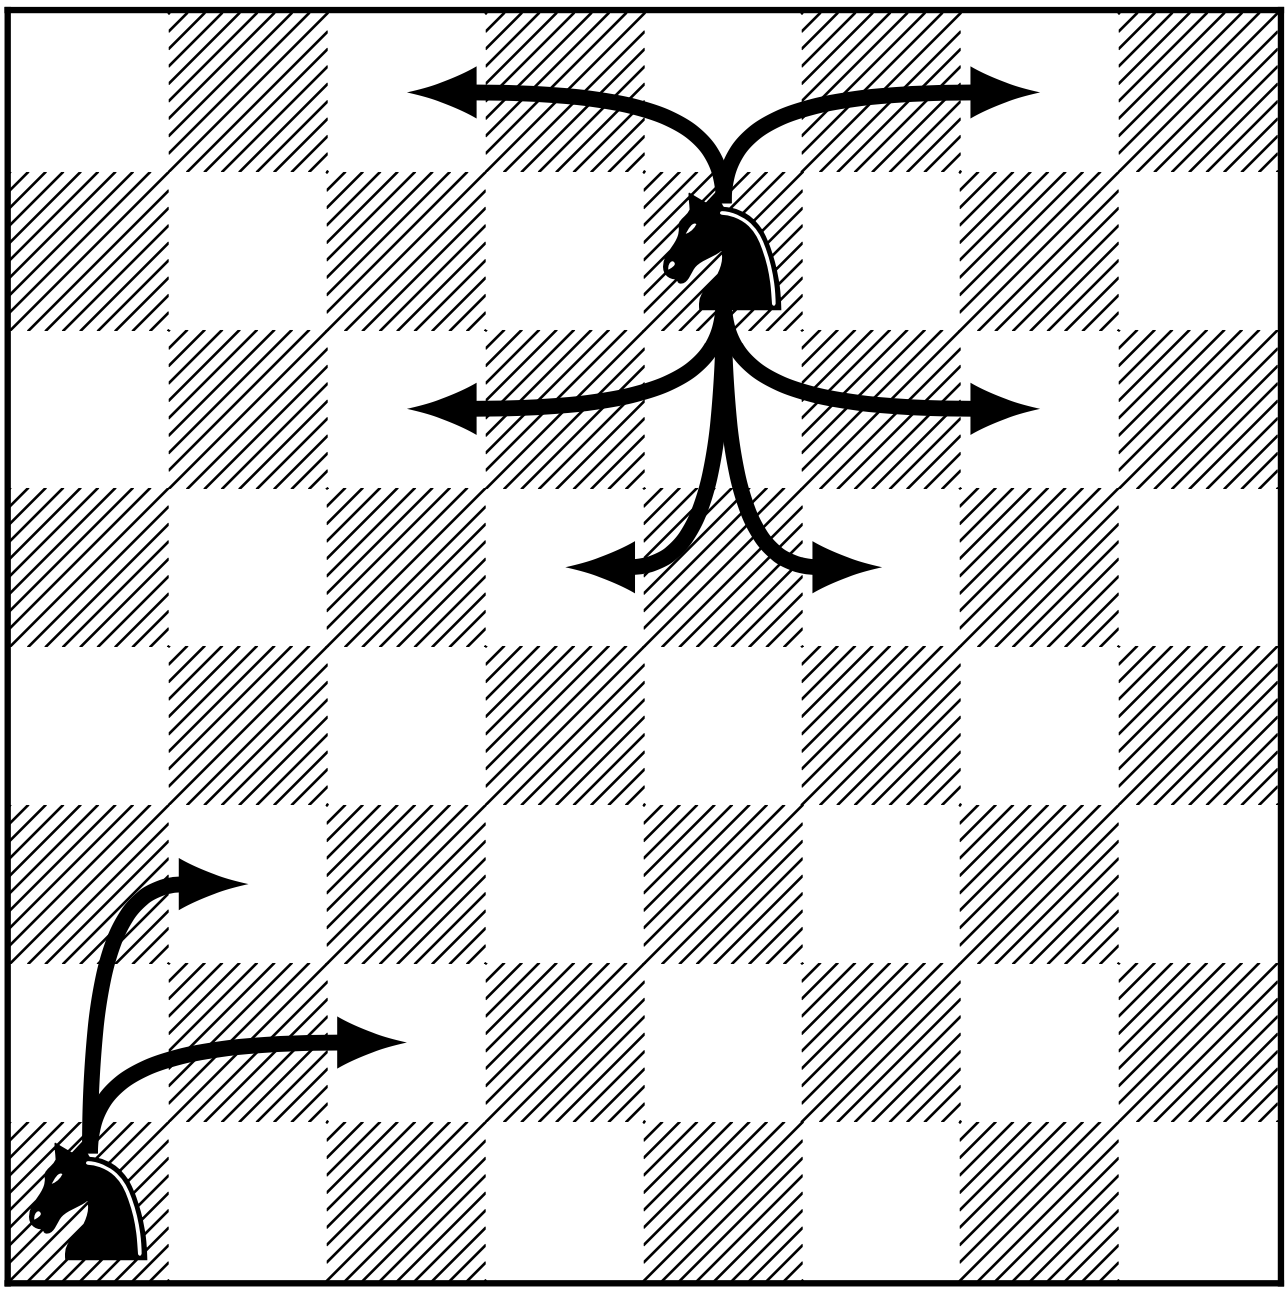
\includegraphics[width=0.35\linewidth,style="float:right; padding:10px"]{pics/knight1} \end{center}

\textbf{Question 4.}
A knight starts in the lower left corner of the chess board and starts moving ``randomly''. That means that from any position, it chooses one of the possible (legal) moves and takes it, with all legal moves having the same probability. It keeps doing the same thing until it comes back to the square it started from.

\begin{enumerate}
\def\labelenumi{\arabic{enumi}.}
\tightlist
\item
  What is the expected number of moves the knight will make before it returns to ``square one''?
\item
  How about the same problem, but using a different chess piece? Which one do you think will come back is the smallest (expected) number of steps?
\item
  (*) How about the same problem, but until \emph{all} squares have been visited at least once?
\end{enumerate}

\textbf{Question 5.} How does Google search work?

\hypertarget{intro}{%
\chapter{An intro to R and RStudio}\label{intro}}

\hypertarget{setting-up-an-r-environment-on-your-computer}{%
\section{Setting up an R environment on your computer}\label{setting-up-an-r-environment-on-your-computer}}

\hypertarget{installing-r}{%
\subsection{Installing R}\label{installing-r}}

Learning basic R is an important part of this course, and the first order of business is to download and install an R distribution on your personal computer. We will be using RStudio as an IDE (integrated development environment). Like R itself, it is free and readily available for all major platforms. To download R to your computer, go to
\url{https://cloud.r-project.org} and
download the version of R for your operating system (Windows, Mac or Linux). If you are on a Mac, you want the ``Latest release'' which, at the time of writing, is 4.1.1, with code name ``Kick Things''. On Windows, follow the link ``install R for the first time''. We are not going to do any cutting edge stuff in this class, so an older release should be fine, too, if you happen to have it already installed on your system. Once you download the installation file (.pkg on a Mac or .exe on Windows), run it and follow instructions. If you are running Linux, you don't need me to tell you what to do. Once it is successfully installed, \textbf{don't run the installed app}. We will use RStudio for that.

\hypertarget{installing-rstudio}{%
\subsection{Installing RStudio}\label{installing-rstudio}}

To install RStudio, go to \url{https://rstudio.com/products/rstudio/download/}. There are several versions to choose from - the one you are looking for is ``RStudio desktop - Free''. After you download and install it, you are ready to run it. When it opens, you will see something like this

\begin{center}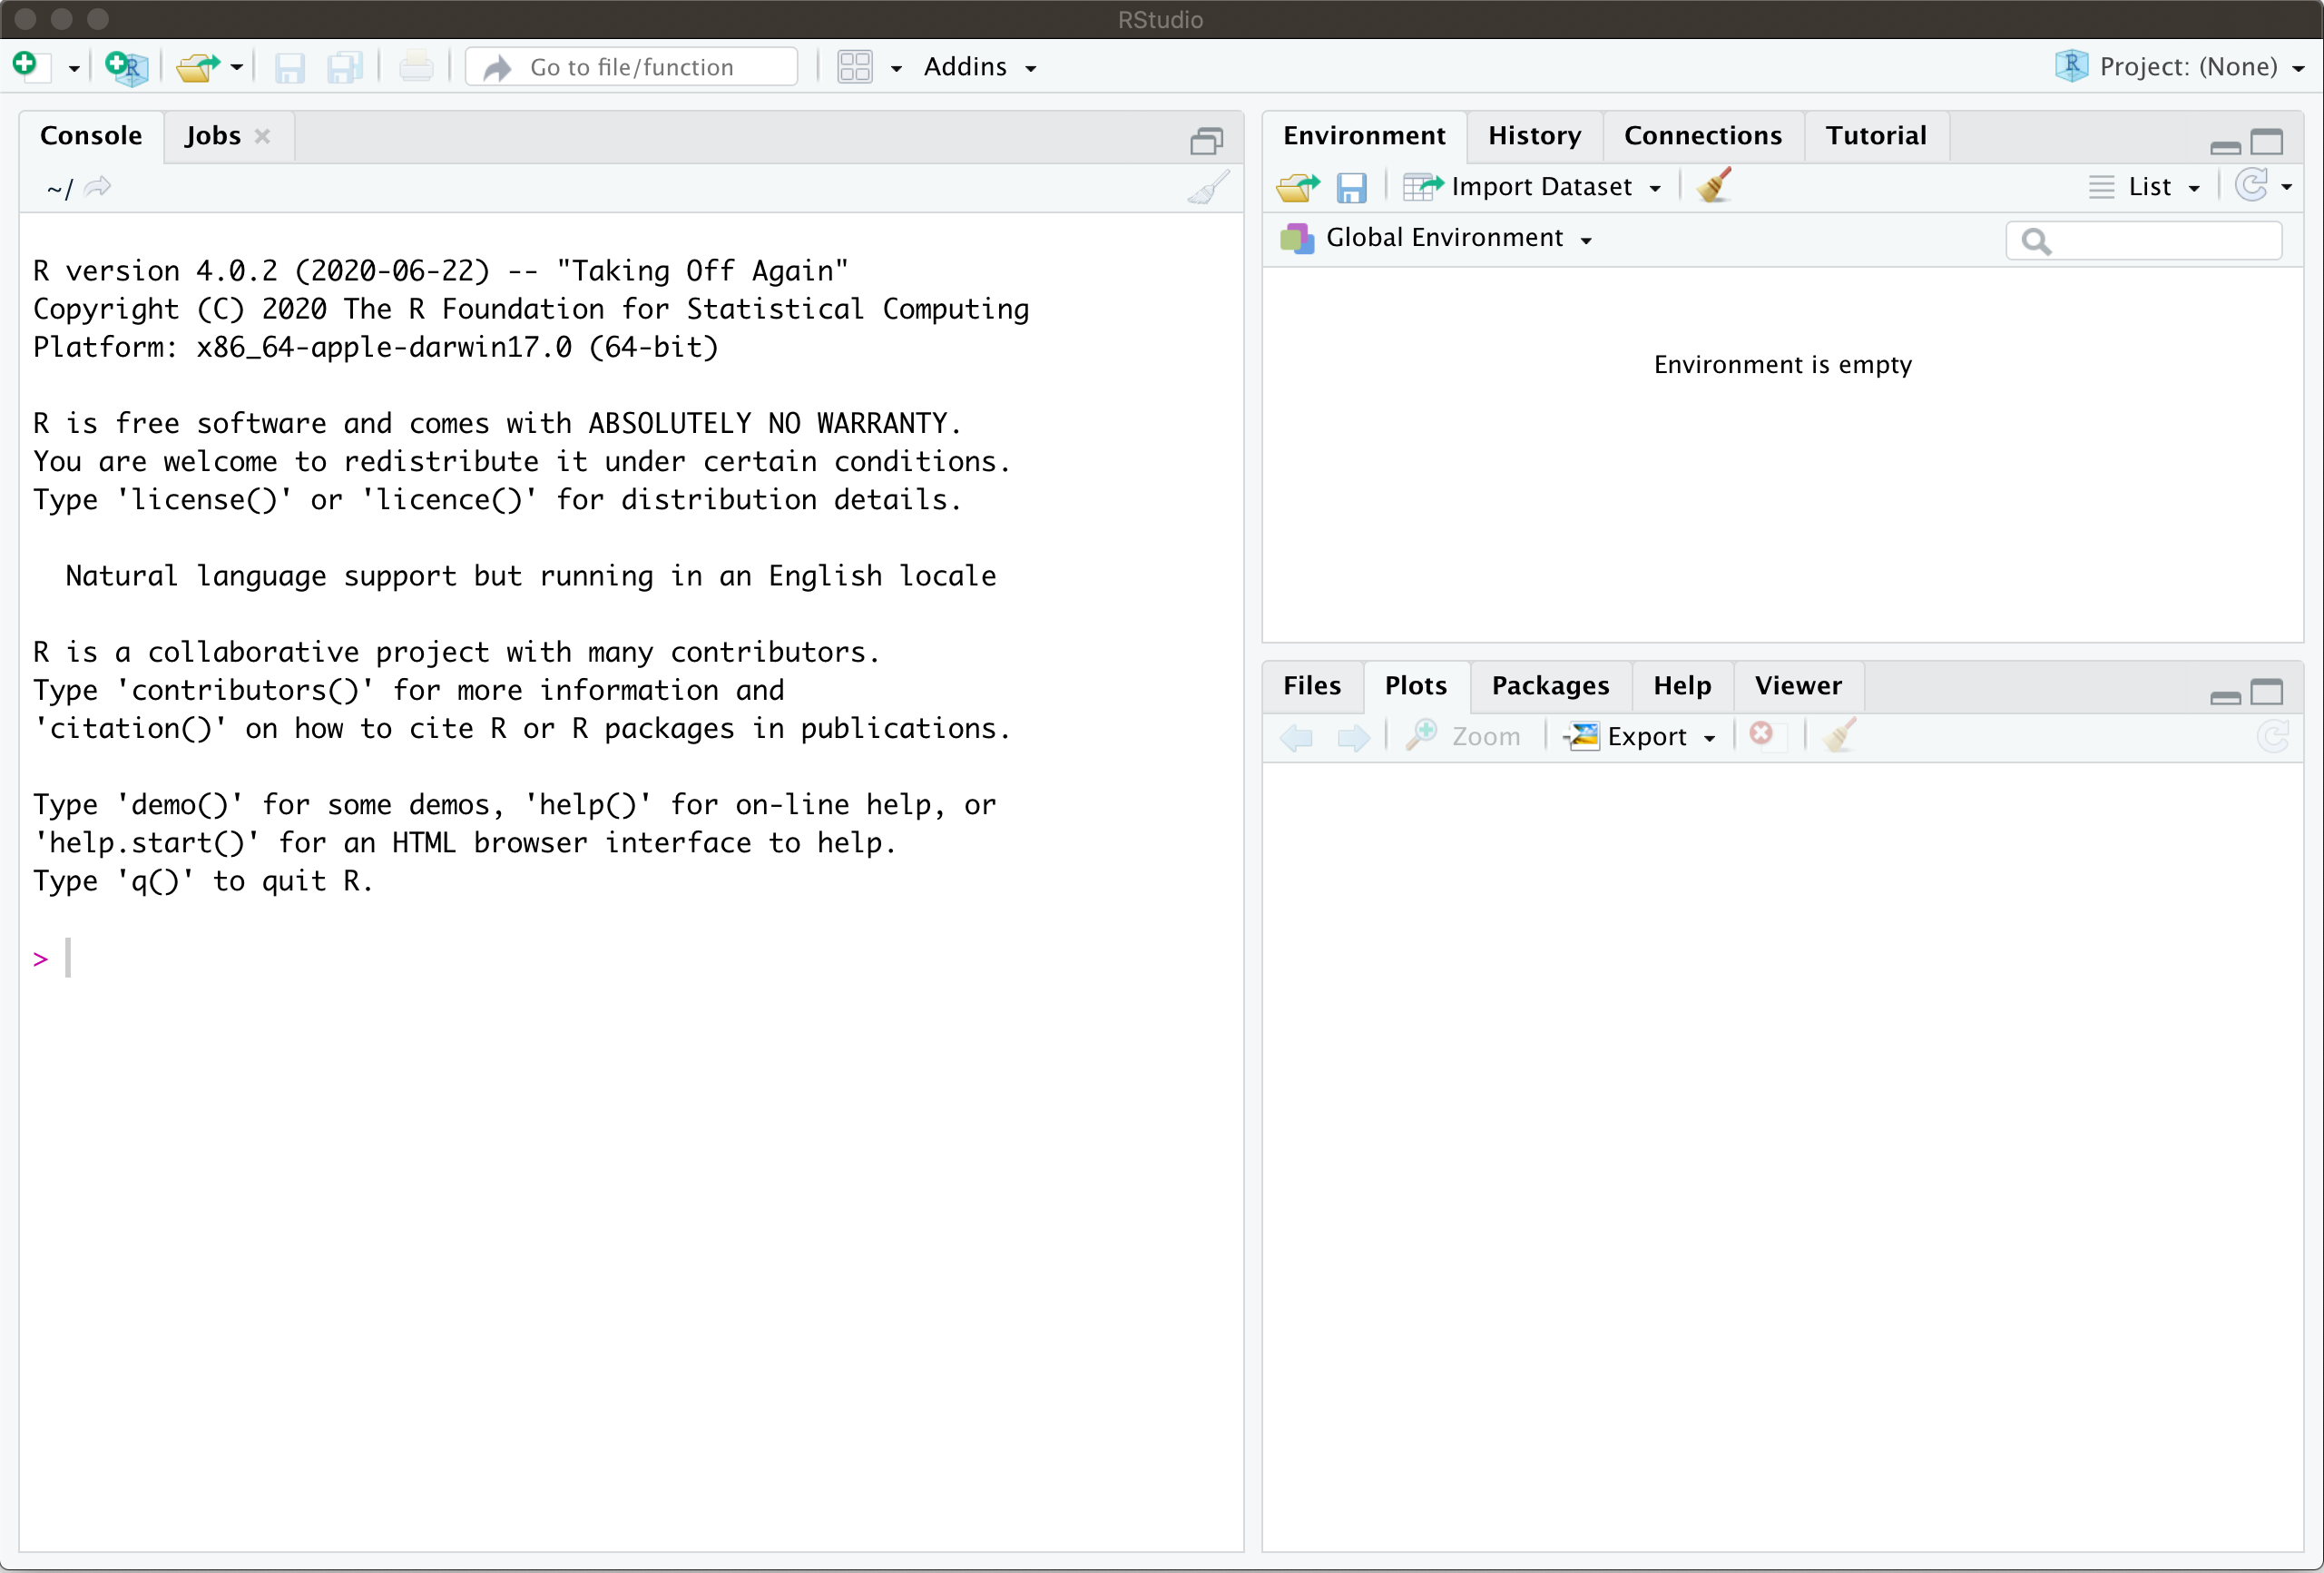
\includegraphics[width=1\linewidth,style="padding:10px"]{pics/RStudio_IDE} \end{center}

The part on the left is called the \emph{console} and that is (one of the places) where you enter commands. Before you do, it is important to adjust a few settings. Open the options window by navigating to to Tools-\textgreater Global Options. In there, uncheck ``Restore .RData into workspace on startup'' and set ``Save workspace to .RData on exit'' to ``Never'', as shown below:

\begin{center}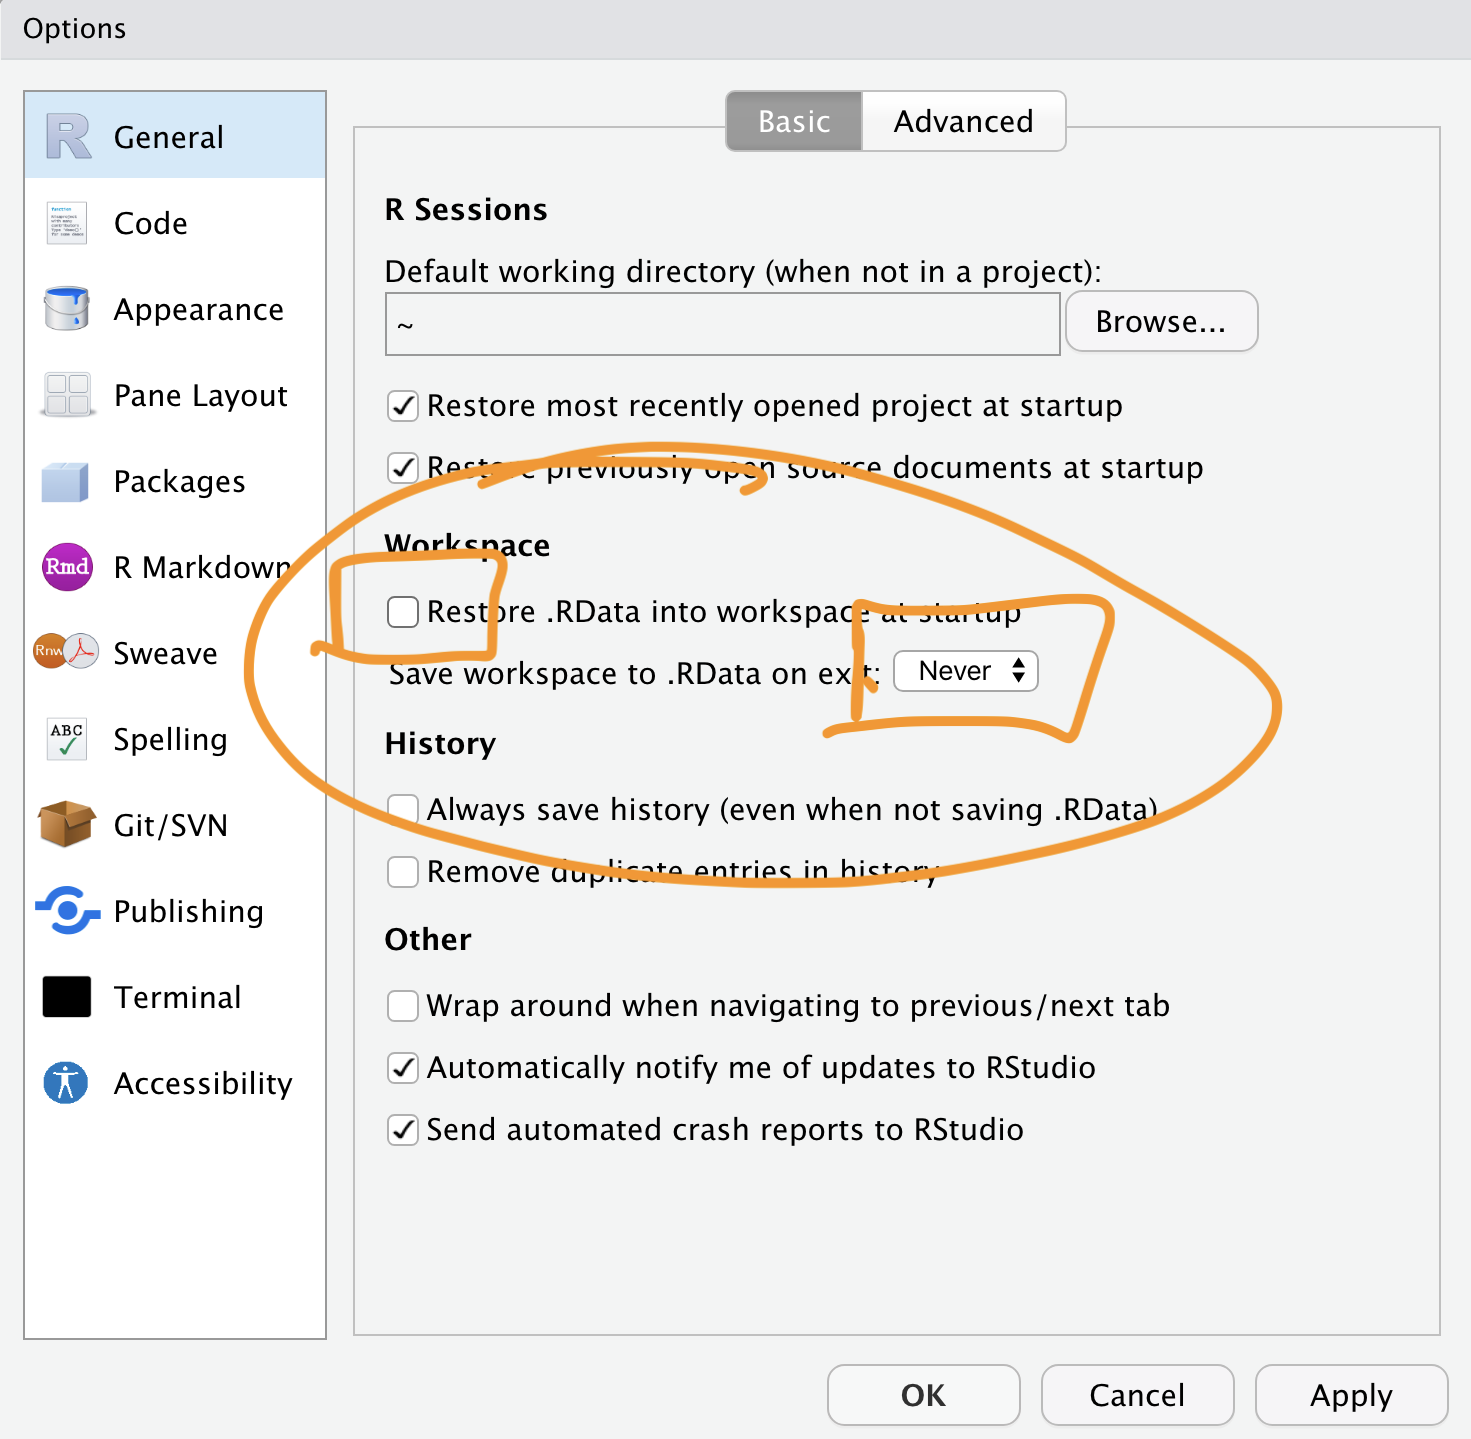
\includegraphics[width=0.75\linewidth,style="margin-left: 12.5%; margin-right:12.5%; padding:10px"]{pics/Restore_RData} \end{center}

This way, R will not pollute your environment with values you defined two weeks ago and completely forgot about. These settings are really an atavism and serve no purpose (for users like us) other than to introduce hard-to-track bugs. 

There are many other settings you can play with in RStudio, but the two I mentioned above are the only ones that I really recommend setting as soon as you install it. 


### Installing basic packages

Finally, we need to install several R packages we will be using (mostly implicitly) during the class. First, run the following command in your console
```markdown
install.packages( "tidyverse")
```
If R asks "Do you want to install from sources the packages which need compilation? (Yes/no/cancel)" answer no.

This will install a number of useful packages and should only take about a minute or two. The next part is a bit longer, and can take up to 15 minutes if you have a slow computer/internet connection.
You only have to do it once, though. Skip both steps involving `tinytex` below if you have LaTeX already installed on your system^[it may interfere with your existing installation].  Start with 
```markdown
install.packages("tinytex")
```
followed by 

```markdown
tinytex::install_tinytex()
```
Note that if you go to the top right corner of each of the code blocks (gray boxes) containing instructions above, an icon will appear. If you click on it, it will copy the content of the box into your clipboard, and you can simply paste it into RStudio. You can do that with any code block in these notes.

## Learning the  basics of R

Once R and RStudio are on your computer, it is time to get acquainted with the basics of R. This class is not about the finer points of R itself, and I will try to make your R experience as smooth as possible. After all, R is a tool that will help us explore and understand stochastic processes. Having said  that, it is important to realize that R is a powerful programming language specifically created for statistical and probabilistic applications. Some knowledge of R is a valuable skill to have in today's job market, and you should take this opportunity to learn it. The best way, of course, is by using it, but before you start, you need to know the very basics. Don't worry, R is very user friendly and easy to get started in. In addition, it has been around for a long time (its predecessor S appeared in 1976) and is extremely well documented -  google *introduction to R* or a similar phrase, and you will get lots of useful hits. 

My plan is to give you a bare minimum in the next few paragraphs, and then to explain additional R concepts as we need them. This way, you will not be overwhelmed right from the start, and you will get a bit of a mathematical context as you learn more. Conversely, learning R commands will help with the math, too.

### The console, Scripts and R Notebooks

There at least  three different ways of inputting commands into R - through console, scripts and R-notebooks.  

**The console**, as I already mentioned, is a window in RStudio where you can enter your R commands one by one. As a command is entered (and enter pressed) R will run it and display the result below. A typical console session looks like this

\begin{center}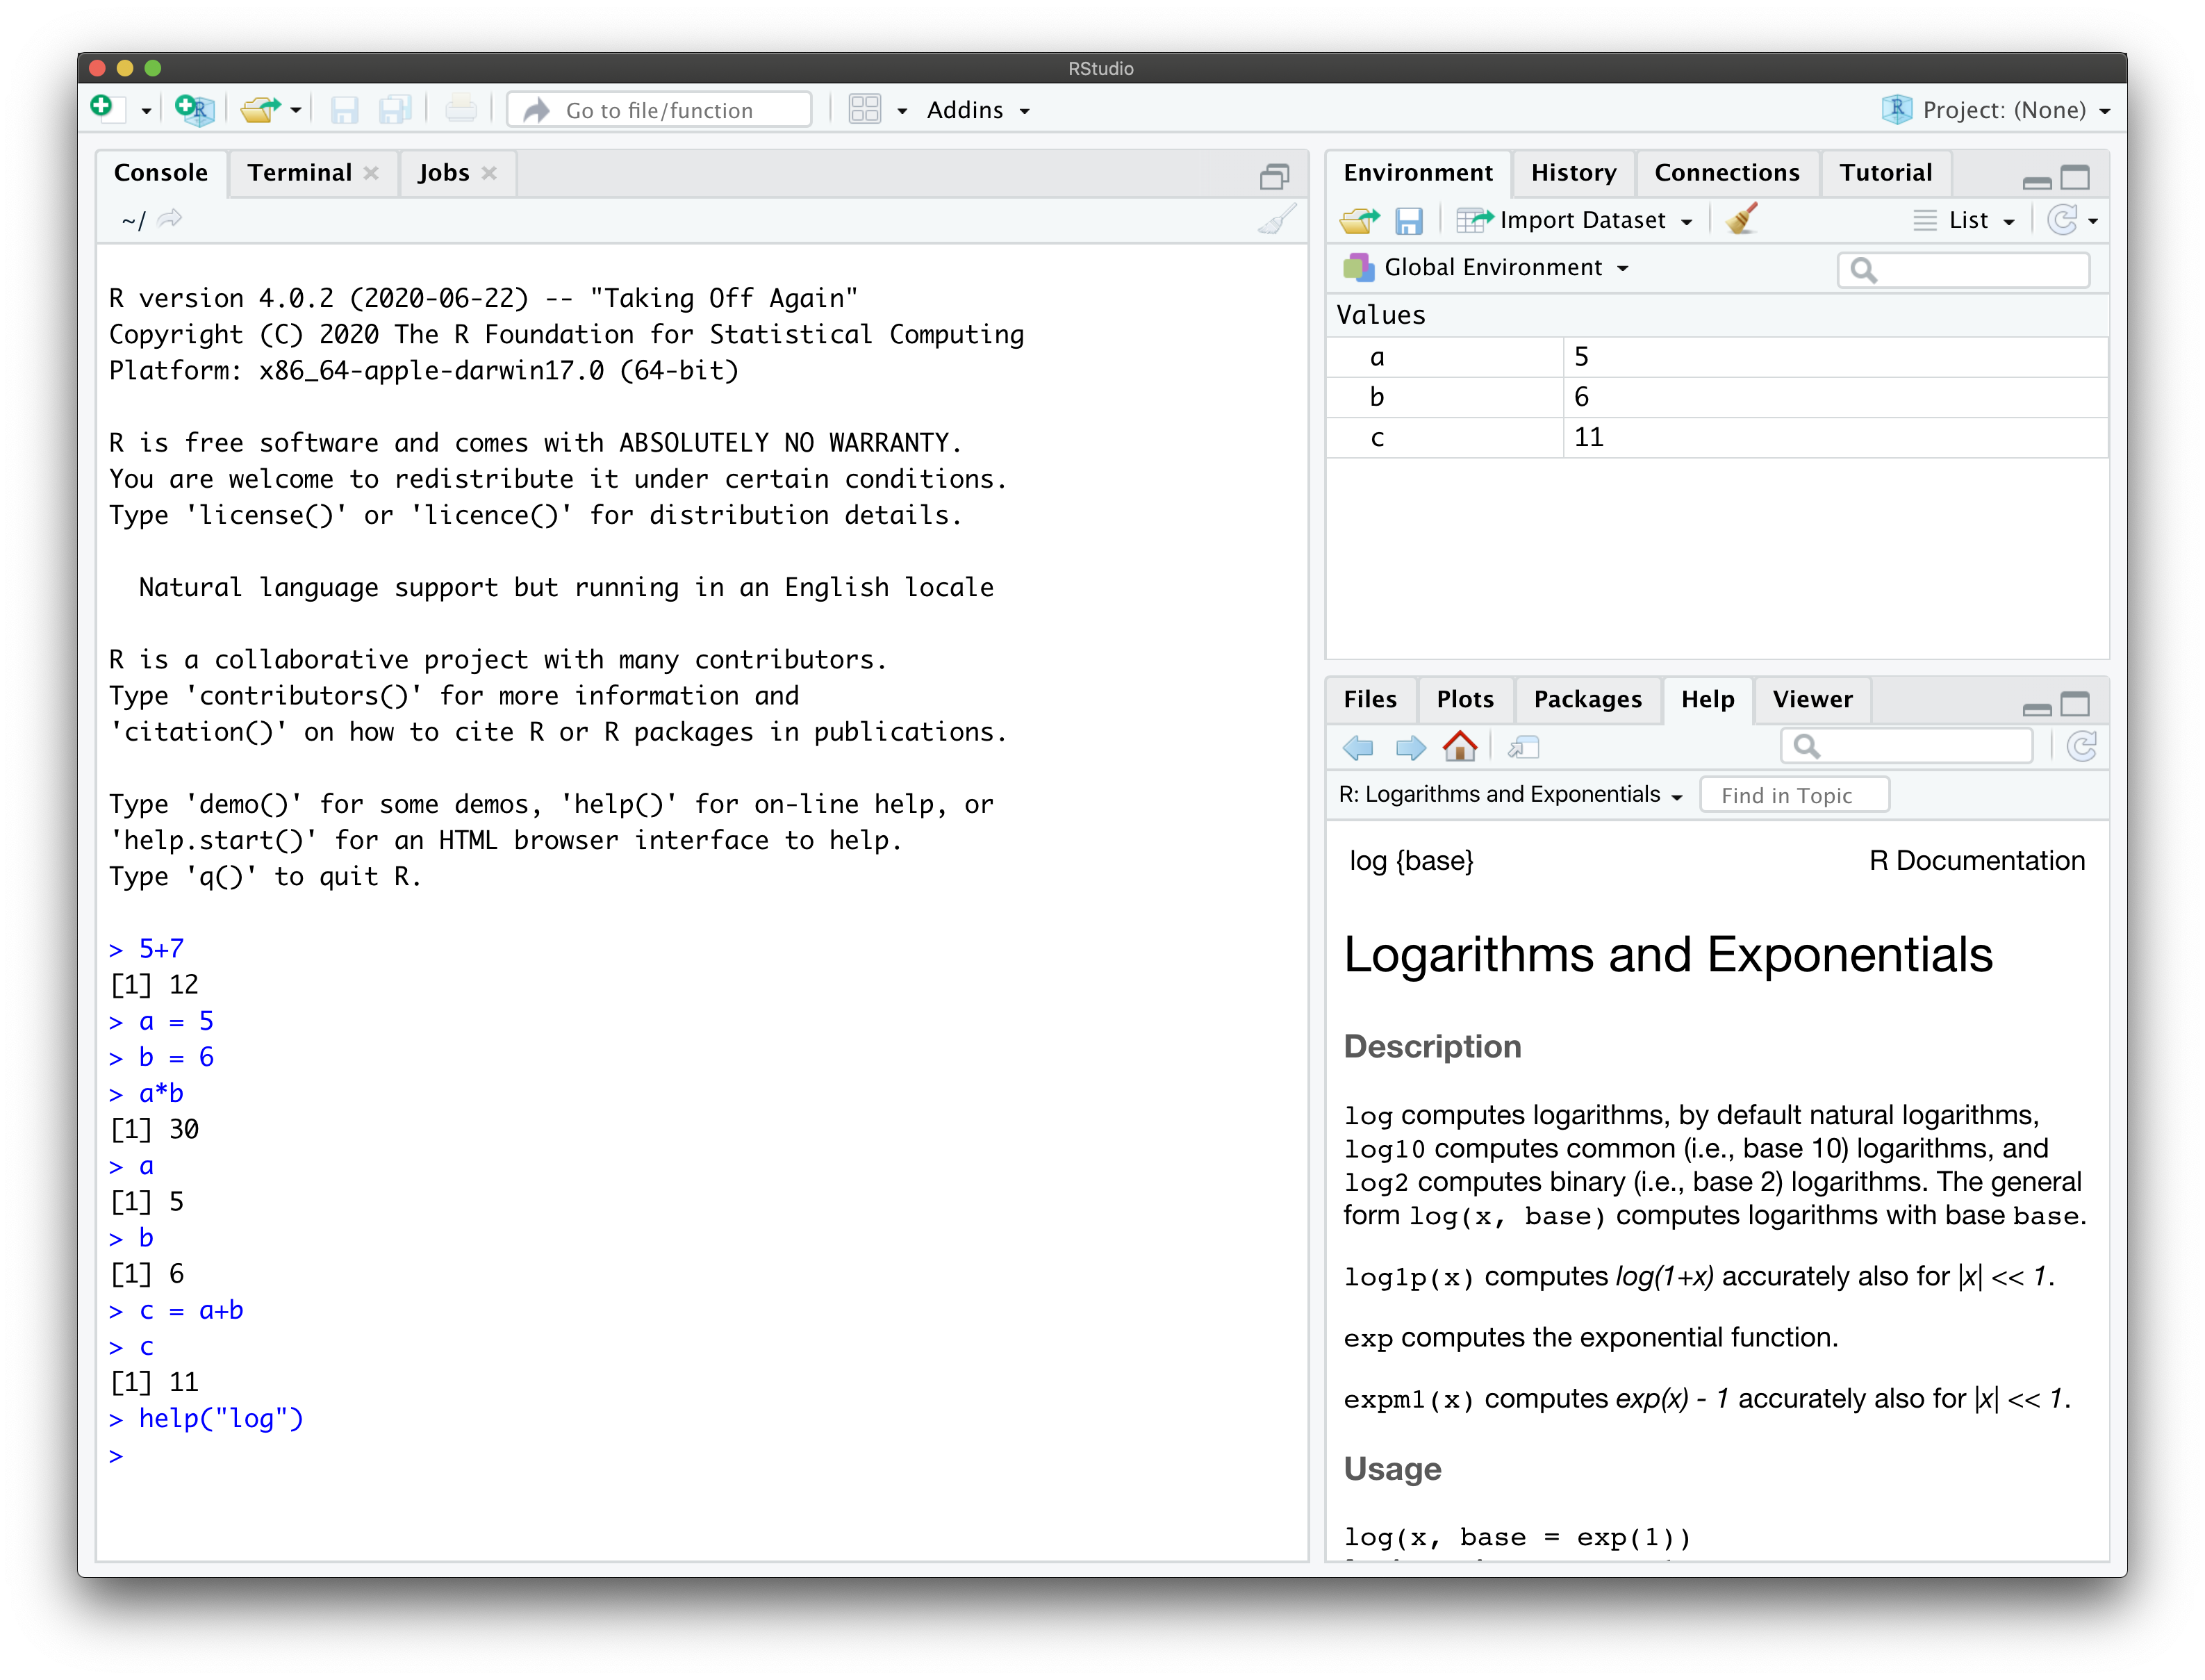
\includegraphics[width=1\linewidth,style="padding:10px"]{pics/console_session} \end{center}

If you define a variable in a command, it will be available in all the subsequent commands. This way of interacting with R is perfect for quick-and-dirty computations and, what is somewhat euphemistically called ``prototyping''. In other words, this way you are using R as a calculator. There is another reason why you might be using the console. It is perfect for package installation and for help-related commands. If you type \texttt{help(\textquotesingle{}log\textquotesingle{})}, the output will appear in the \texttt{Help} pane on the right. You can also see all the available variables in the \texttt{Environment} pane on the (top) right.

As your needs increase, you will need more complex (and longer) code to meet them. This is where \textbf{scripts} come in. They are text files (but have the extension \texttt{.R}) that hold R code. Scripts can run as a whole, and be saved for later. To create a new script, go to File-\textgreater New File-\textgreater R Script. That will split your RStudio window in two:

\begin{center}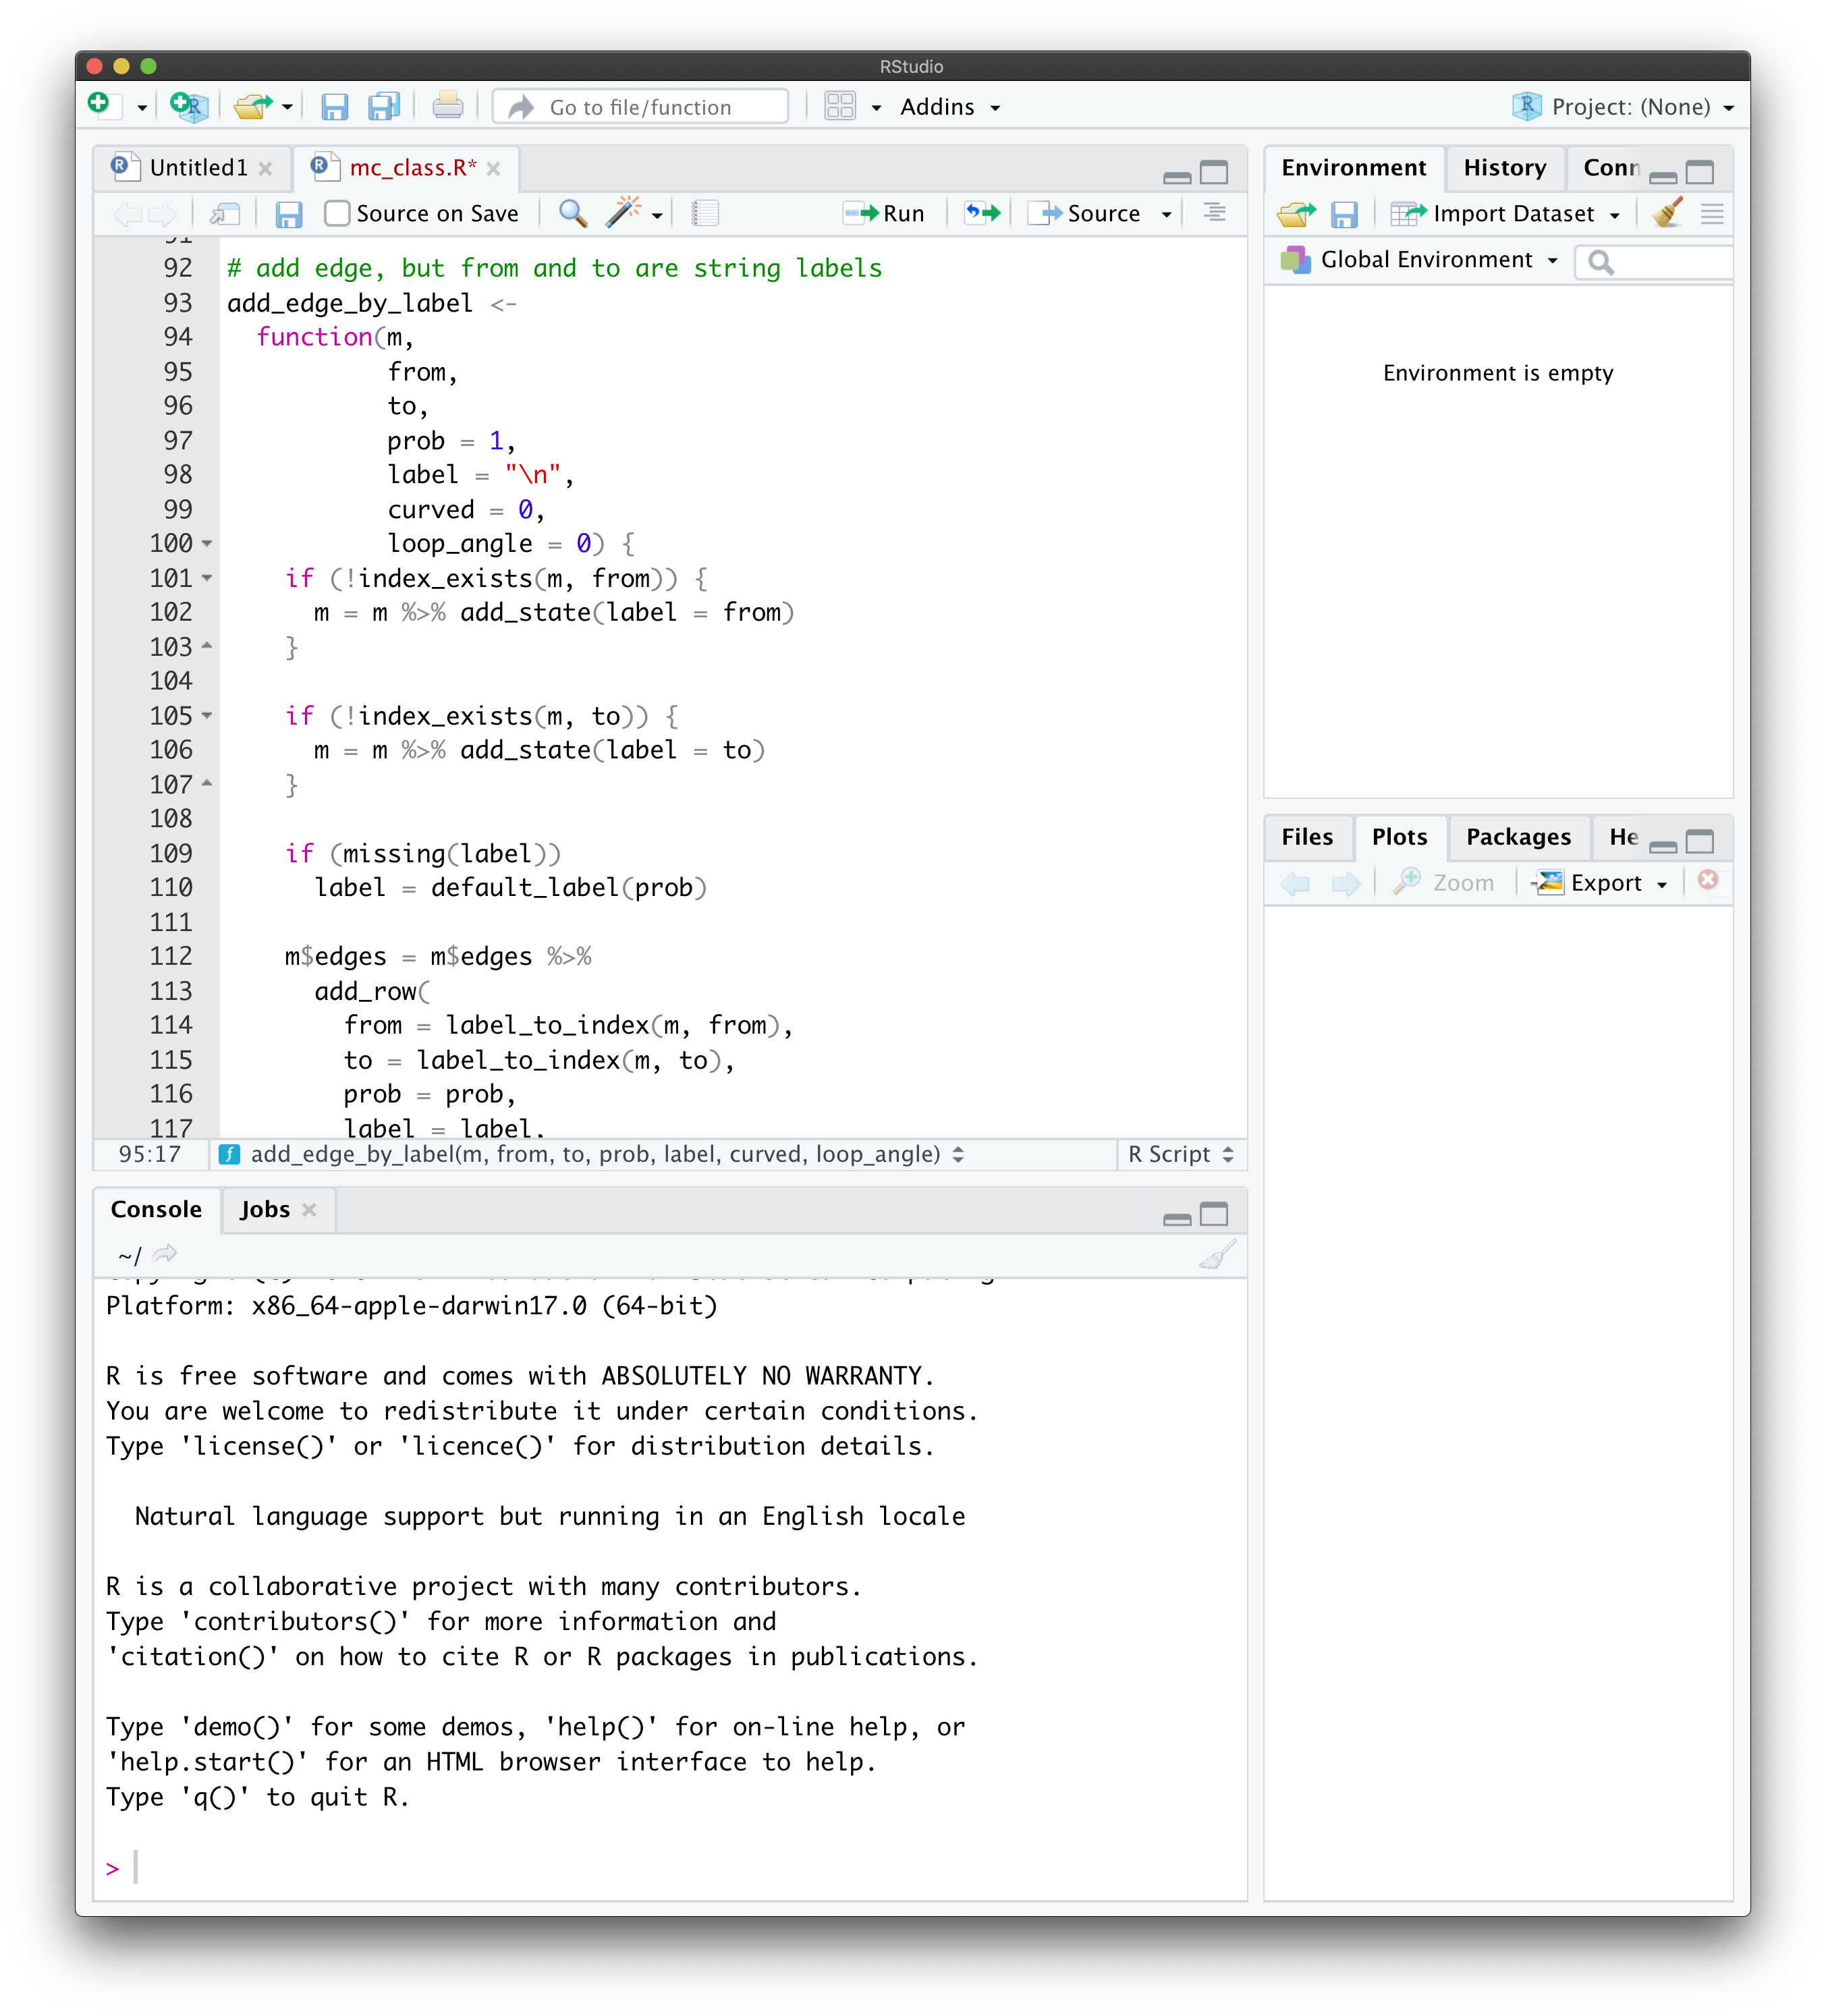
\includegraphics[width=1\linewidth,style="padding:10px"]{pics/script_console} \end{center}

The top part will become a script editor, and your console will shrink to occupy the bottom part. You can write you code in there, edit and update it, and then run the whole script by clicking on Source, or pressing the associated shortcut key.

Inspired by Python Jupyter notebooks, \textbf{R notebooks} are a creature somewhere between scripts and the console, but also have some features of their own.
An R notebook is nothing other than a specially formatted text file which contains \emph{chunks} of R code mixed with regular text. You can think of these chunks as mini scripts. What differentiates them from scripts is that chunks can be executed (evaluated) and the output becomes a part of the notebook:

\begin{center}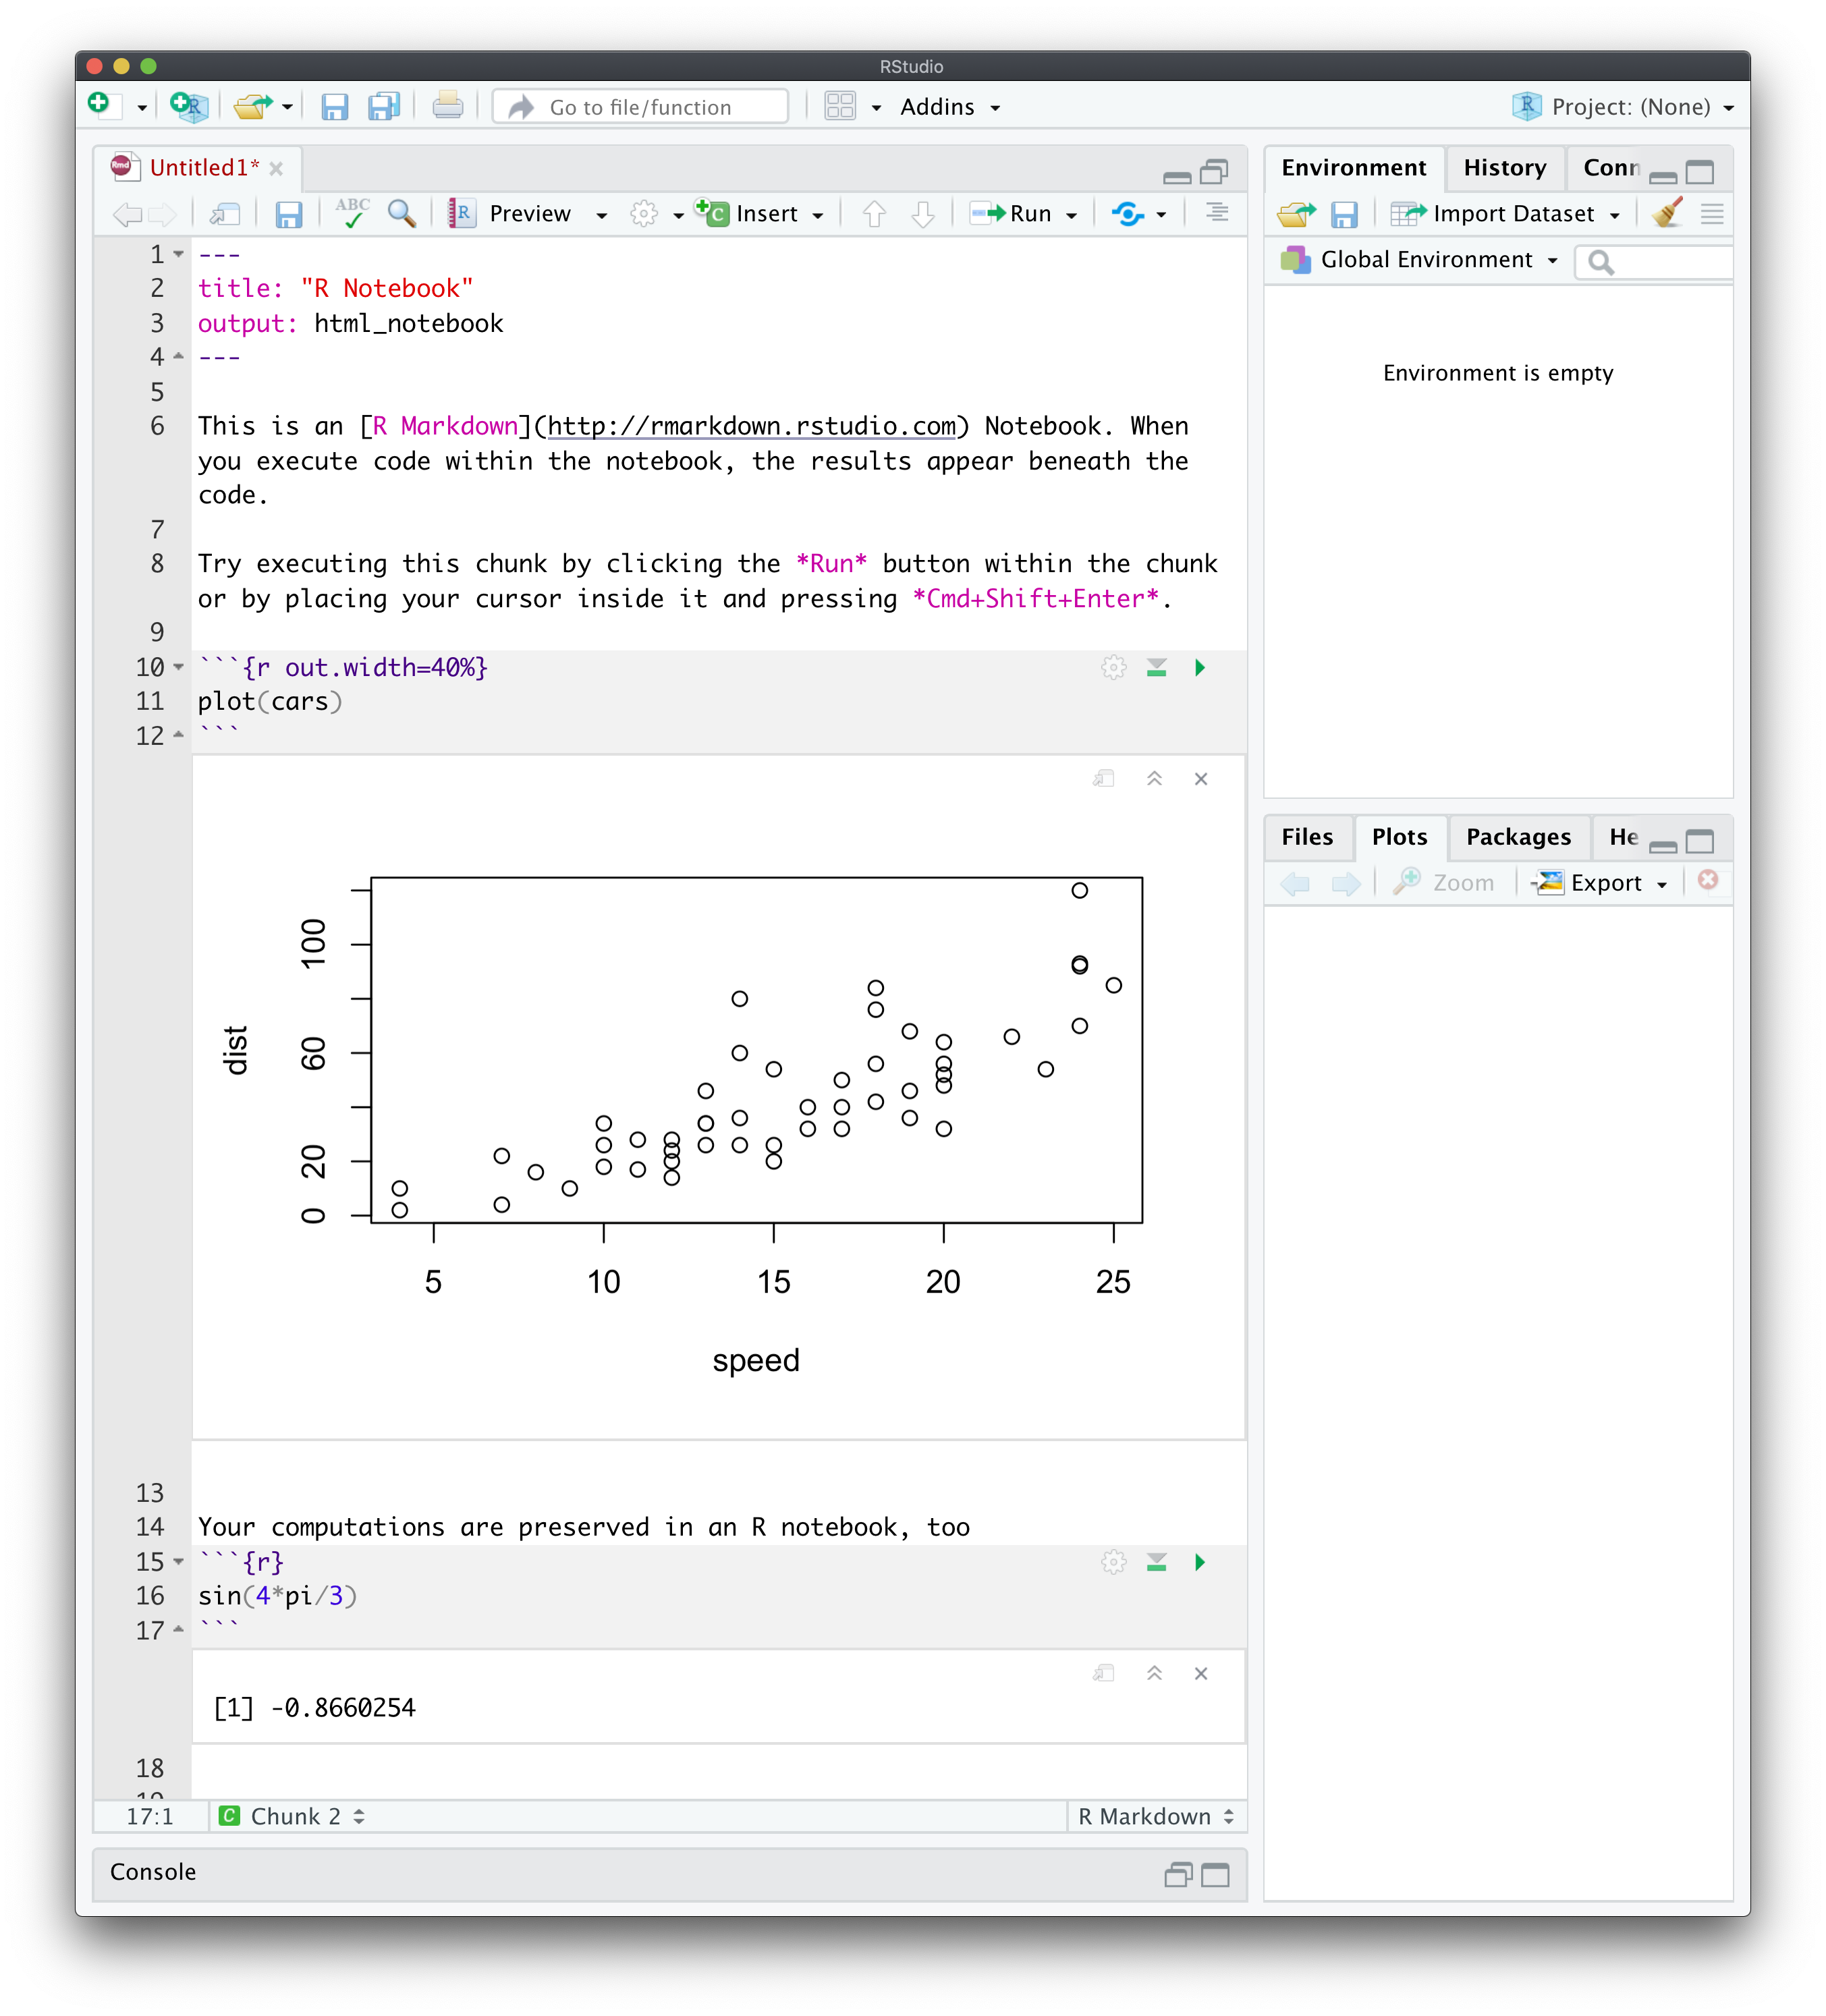
\includegraphics[width=1\linewidth,style="padding:10px"]{pics/notebooks} \end{center}

R notebooks are R's implementation of \emph{literate programming}. The idea is that documentation should be written at the same time as the program itself. As far as this course is concerned, R notebooks are just the right medium for homework and exam submission. You can run code and provide the interpretation of its output in a single document. See \href{other/Homework-instructions.html}{here} for more information.

Each chapter in these lecture notes is an R notebook!

\hypertarget{asking-for-help}{%
\subsection{Asking for help}\label{asking-for-help}}

The most important thing about \textbf{learning R} (and many other things, for that matter) is knowing whom (and how) to ask for help. Luckily, R is a well established language, and you can get a lot of information by simply googling your problem. For example, if you google \texttt{logarithm\ in\ R} the top hit (at the time of writing) gives a nice overview and some examples.

Another way to get information about a command or a concept in R is to use the command \texttt{help}. For example, if you input \texttt{help("log")} or \texttt{?log} in your console, the right hand of your screen will display information on the function \texttt{log} and some of its cousins. Almost every help entry has examples at the bottom, and that is where I always go first.

\hypertarget{vectors}{%
\subsection{Vectors}\label{vectors}}

Objects we will be manipulating in this class are almost exclusively vectors and matrices. The simplest vectors are those that have a single component, in other words, numbers. In R, you can assign a number to a variable using two different notations. Both

\begin{Shaded}
\begin{Highlighting}[]
\NormalTok{a }\OtherTok{\textless{}{-}} \DecValTok{1}
\end{Highlighting}
\end{Shaded}

and

\begin{Shaded}
\begin{Highlighting}[]
\NormalTok{a }\OtherTok{=} \DecValTok{1}
\end{Highlighting}
\end{Shaded}

will assign the value \(1\) to the variable \texttt{a}. If you want to create a longer vector, you can use the \textbf{concatenation operator} \texttt{c} as follows:

\begin{Shaded}
\begin{Highlighting}[]
\NormalTok{x }\OtherTok{=} \FunctionTok{c}\NormalTok{(}\DecValTok{1}\NormalTok{, }\DecValTok{2}\NormalTok{, }\DecValTok{3}\NormalTok{, }\DecValTok{4}\NormalTok{)}
\end{Highlighting}
\end{Shaded}

Once you evaluate the above in your console, the value of \texttt{x} is stored and you can access it by using the command \texttt{print}

\begin{Shaded}
\begin{Highlighting}[]
\FunctionTok{print}\NormalTok{(x)}
\DocumentationTok{\#\# [1] 1 2 3 4}
\end{Highlighting}
\end{Shaded}

or simply evaluating \texttt{x} itself:

\begin{Shaded}
\begin{Highlighting}[]
\NormalTok{x}
\DocumentationTok{\#\# [1] 1 2 3 4}
\end{Highlighting}
\end{Shaded}

Unlike all code blocks above them, the last two contain both input and output. It is standard not to mark the output by any symbol (like the usual \texttt{\textgreater{}}), and to mark the output by \texttt{\#\#} which otherwise marks comments. This way, you can copy any code block from these notes and paste it into the console (or your script) without having to modify it in any way. Try it!

We built the vector \texttt{x} above by concatenating four numbers (vectors of length 1). You can concatenate vectors of different sizes, too:

\begin{Shaded}
\begin{Highlighting}[]
\NormalTok{a }\OtherTok{=} \FunctionTok{c}\NormalTok{(}\DecValTok{1}\NormalTok{, }\DecValTok{2}\NormalTok{, }\DecValTok{3}\NormalTok{)}
\NormalTok{b }\OtherTok{=} \FunctionTok{c}\NormalTok{(}\DecValTok{4}\NormalTok{, }\DecValTok{5}\NormalTok{, }\DecValTok{6}\NormalTok{)}
\NormalTok{(}\AttributeTok{x =} \FunctionTok{c}\NormalTok{(a, b, }\DecValTok{7}\NormalTok{))}
\DocumentationTok{\#\# [1] 1 2 3 4 5 6 7}
\end{Highlighting}
\end{Shaded}

You may be wondering why I put \texttt{x\ =\ c(a,b,7)} in parentheses. Without them, \texttt{x} would still become (1,2,3,4,5,6,7), but its value would not be printed out. A statement in parentheses is not only evaluated, but its result is also printed out. This way, \texttt{(x\ =\ 2+3)} is equivalent to \texttt{x\ =\ 2+3} followed by \texttt{x} or \texttt{print(x)}.

Vectors can contain things other than numbers. Strings, for example:

\begin{Shaded}
\begin{Highlighting}[]
\NormalTok{(}\AttributeTok{x =} \FunctionTok{c}\NormalTok{(}\StringTok{"Picard"}\NormalTok{, }\StringTok{"Data"}\NormalTok{, }\StringTok{"Geordi"}\NormalTok{))}
\DocumentationTok{\#\# [1] "Picard" "Data"   "Geordi"}
\end{Highlighting}
\end{Shaded}

If you need a vector consisting of consecutive numbers, use the colon \texttt{:} notation:

\begin{Shaded}
\begin{Highlighting}[]
\DecValTok{1}\SpecialCharTok{:}\DecValTok{10}
\DocumentationTok{\#\#  [1]  1  2  3  4  5  6  7  8  9 10}
\end{Highlighting}
\end{Shaded}

For sequences of equally spaced numbers, use the command \texttt{seq} (check its help for details)

\begin{Shaded}
\begin{Highlighting}[]
\FunctionTok{seq}\NormalTok{(}\AttributeTok{from =} \DecValTok{5}\NormalTok{, }\AttributeTok{to =} \DecValTok{20}\NormalTok{, }\AttributeTok{by =} \DecValTok{3}\NormalTok{)}
\DocumentationTok{\#\# [1]  5  8 11 14 17 20}
\end{Highlighting}
\end{Shaded}

An important feature or R is that many of its functions are \textbf{vectorized}. That means that if you give such a function a vector as an argument, the returned value will be a vector of results of that operation performed element by element. For example

\begin{Shaded}
\begin{Highlighting}[]
\NormalTok{x }\OtherTok{=} \FunctionTok{c}\NormalTok{(}\DecValTok{10}\NormalTok{, }\DecValTok{20}\NormalTok{, }\DecValTok{30}\NormalTok{)}
\NormalTok{y }\OtherTok{=} \FunctionTok{c}\NormalTok{(}\DecValTok{2}\NormalTok{, }\DecValTok{4}\NormalTok{, }\DecValTok{5}\NormalTok{)}
\NormalTok{x }\SpecialCharTok{+}\NormalTok{ y}
\DocumentationTok{\#\# [1] 12 24 35}
\NormalTok{x }\SpecialCharTok{*}\NormalTok{ y}
\DocumentationTok{\#\# [1]  20  80 150}
\NormalTok{x}\SpecialCharTok{\^{}}\DecValTok{2}
\DocumentationTok{\#\# [1] 100 400 900}
\FunctionTok{cos}\NormalTok{(x)}
\DocumentationTok{\#\# [1] {-}0.8390715  0.4080821  0.1542514}
\end{Highlighting}
\end{Shaded}

The vectors do not need to be of the same size. R uses the \textbf{recycling rule} -
it recycles the values of the shorter one, starting from the beginning, until
its size matches the longer one:

\begin{Shaded}
\begin{Highlighting}[]
\NormalTok{x }\OtherTok{=} \FunctionTok{c}\NormalTok{(}\DecValTok{10}\NormalTok{, }\DecValTok{20}\NormalTok{, }\DecValTok{30}\NormalTok{, }\DecValTok{40}\NormalTok{, }\DecValTok{50}\NormalTok{, }\DecValTok{60}\NormalTok{)}
\NormalTok{y }\OtherTok{=} \FunctionTok{c}\NormalTok{(}\DecValTok{1}\NormalTok{, }\DecValTok{3}\NormalTok{)}
\NormalTok{x }\SpecialCharTok{+}\NormalTok{ y}
\DocumentationTok{\#\# [1] 11 23 31 43 51 63}
\end{Highlighting}
\end{Shaded}

The case where the shorter vector is of length 1 is particularly useful:

\begin{Shaded}
\begin{Highlighting}[]
\NormalTok{x }\OtherTok{=} \FunctionTok{c}\NormalTok{(}\DecValTok{10}\NormalTok{, }\DecValTok{20}\NormalTok{, }\DecValTok{30}\NormalTok{, }\DecValTok{40}\NormalTok{)}
\NormalTok{x }\SpecialCharTok{+} \DecValTok{1}
\DocumentationTok{\#\# [1] 11 21 31 41}
\NormalTok{x }\SpecialCharTok{*}\NormalTok{ (}\SpecialCharTok{{-}}\DecValTok{2}\NormalTok{)}
\DocumentationTok{\#\# [1] {-}20 {-}40 {-}60 {-}80}
\end{Highlighting}
\end{Shaded}

Extracting parts of the vector is accomplished by using the \textbf{indexing} operator \texttt{{[}{]}}. Here are some examples (what do negative numbers do?)

\begin{Shaded}
\begin{Highlighting}[]
\NormalTok{x }\OtherTok{=} \FunctionTok{c}\NormalTok{(}\DecValTok{10}\NormalTok{, }\DecValTok{20}\NormalTok{, }\DecValTok{30}\NormalTok{, }\DecValTok{40}\NormalTok{, }\DecValTok{50}\NormalTok{)}
\NormalTok{x[}\DecValTok{1}\NormalTok{]}
\DocumentationTok{\#\# [1] 10}
\NormalTok{x[}\FunctionTok{c}\NormalTok{(}\DecValTok{1}\NormalTok{, }\DecValTok{2}\NormalTok{)]}
\DocumentationTok{\#\# [1] 10 20}
\NormalTok{x[}\SpecialCharTok{{-}}\DecValTok{1}\NormalTok{]}
\DocumentationTok{\#\# [1] 20 30 40 50}
\NormalTok{x[}\SpecialCharTok{{-}}\FunctionTok{c}\NormalTok{(}\DecValTok{3}\NormalTok{, }\DecValTok{4}\NormalTok{)]}
\DocumentationTok{\#\# [1] 10 20 50}
\NormalTok{x[}\DecValTok{1}\SpecialCharTok{:}\DecValTok{4}\NormalTok{]}
\DocumentationTok{\#\# [1] 10 20 30 40}
\NormalTok{x[}\FunctionTok{c}\NormalTok{(}\DecValTok{1}\NormalTok{, }\DecValTok{1}\NormalTok{, }\DecValTok{2}\NormalTok{, }\DecValTok{2}\NormalTok{, }\DecValTok{5}\NormalTok{, }\DecValTok{4}\NormalTok{)]}
\DocumentationTok{\#\# [1] 10 10 20 20 50 40}
\end{Highlighting}
\end{Shaded}

People familiar with Python should be aware of the following two differences: 1. indexing starts at 1 and not 0, and 2. negative indexing removes components; it does not start counting from the end!

It is important to note that the thing you put inside \texttt{{[}{]}} needs to be a vector itself. The above examples all dealt with numerical indices, but you can use logical indices, too. A variable is said to be \textbf{logical} or \textbf{Boolean} if it can take only one of the two values \texttt{TRUE} or \texttt{FALSE}. A vector whose components are all logical, are called, of course, logical vectors. You can think of logical indexing as the operation where you go through your original vector, and choose which components you want to keep (\texttt{TRUE}) and which you want the throw away (\texttt{FALSE}). For example

\begin{Shaded}
\begin{Highlighting}[]
\NormalTok{x }\OtherTok{=} \FunctionTok{c}\NormalTok{(}\DecValTok{10}\NormalTok{, }\DecValTok{20}\NormalTok{, }\DecValTok{30}\NormalTok{, }\DecValTok{40}\NormalTok{, }\DecValTok{50}\NormalTok{)}
\NormalTok{y }\OtherTok{=} \FunctionTok{c}\NormalTok{(}\ConstantTok{TRUE}\NormalTok{, }\ConstantTok{FALSE}\NormalTok{, }\ConstantTok{FALSE}\NormalTok{, }\ConstantTok{TRUE}\NormalTok{, }\ConstantTok{TRUE}\NormalTok{)}
\NormalTok{x[y]}
\DocumentationTok{\#\# [1] 10 40 50}
\end{Highlighting}
\end{Shaded}

This is especially useful when used together with the \textbf{comparison operators}. The expressions like \texttt{x\ \textless{}\ y} or \texttt{x\ ==\ y} are operators\footnote{be careful, though. The expression \texttt{x\ =\ y} is not the same as \texttt{x\ ==\ y}. It does not return a logical value - it assigns the value of \texttt{y} to \texttt{x}} in R, just like \texttt{x\ +\ y} or \texttt{x\ /\ y}. The difference is that \texttt{\textless{}} and \texttt{==} return logical values. For example

\begin{Shaded}
\begin{Highlighting}[]
\DecValTok{1} \SpecialCharTok{==} \DecValTok{2}
\DocumentationTok{\#\# [1] FALSE}
\DecValTok{3} \SpecialCharTok{\textgreater{}} \DecValTok{4}
\DocumentationTok{\#\# [1] FALSE}
\DecValTok{3} \SpecialCharTok{\textgreater{}=} \DecValTok{2}
\DocumentationTok{\#\# [1] TRUE}
\end{Highlighting}
\end{Shaded}

These operators are vectorized, so you can do things like this

\begin{Shaded}
\begin{Highlighting}[]
\NormalTok{x }\OtherTok{=} \FunctionTok{c}\NormalTok{(}\DecValTok{1}\NormalTok{, }\DecValTok{2}\NormalTok{, }\DecValTok{3}\NormalTok{, }\DecValTok{4}\NormalTok{, }\DecValTok{5}\NormalTok{)}
\NormalTok{y }\OtherTok{=} \FunctionTok{c}\NormalTok{(}\DecValTok{1}\NormalTok{, }\DecValTok{3}\NormalTok{, }\DecValTok{3}\NormalTok{, }\DecValTok{2}\NormalTok{, }\DecValTok{5}\NormalTok{)}
\NormalTok{x }\SpecialCharTok{==}\NormalTok{ y}
\DocumentationTok{\#\# [1]  TRUE FALSE  TRUE FALSE  TRUE}
\end{Highlighting}
\end{Shaded}

or, using recycling,

\begin{Shaded}
\begin{Highlighting}[]
\NormalTok{x }\OtherTok{=} \FunctionTok{c}\NormalTok{(}\DecValTok{1}\NormalTok{, }\DecValTok{2}\NormalTok{, }\DecValTok{3}\NormalTok{, }\DecValTok{4}\NormalTok{, }\DecValTok{5}\NormalTok{)}
\NormalTok{x }\SpecialCharTok{\textgreater{}} \DecValTok{3}
\DocumentationTok{\#\# [1] FALSE FALSE FALSE  TRUE  TRUE}
\end{Highlighting}
\end{Shaded}

Let's combine that with indexing. Suppose that we want to keep only the values greater than 4 in the vector \texttt{x}. The vector \texttt{y\ =\ (\ x\ \textgreater{}\ 4\ )} is going to be of the same length as \texttt{x} and contain logical values.
When we index \texttt{x} using it, only the values of \texttt{x} on positions where \texttt{x\ \textgreater{}\ 4} will survive, and these are exactly the values we needed:

\begin{Shaded}
\begin{Highlighting}[]
\NormalTok{x }\OtherTok{=} \FunctionTok{c}\NormalTok{(}\DecValTok{3}\NormalTok{, }\DecValTok{2}\NormalTok{, }\DecValTok{5}\NormalTok{, }\DecValTok{3}\NormalTok{, }\DecValTok{1}\NormalTok{, }\DecValTok{5}\NormalTok{, }\DecValTok{6}\NormalTok{, }\DecValTok{4}\NormalTok{)}
\NormalTok{y }\OtherTok{=}\NormalTok{ (x }\SpecialCharTok{\textgreater{}} \DecValTok{4}\NormalTok{)}
\NormalTok{x[y]}
\DocumentationTok{\#\# [1] 5 5 6}
\end{Highlighting}
\end{Shaded}

or, simply,

\begin{Shaded}
\begin{Highlighting}[]
\NormalTok{x[x }\SpecialCharTok{\textgreater{}} \DecValTok{4}\NormalTok{]}
\DocumentationTok{\#\# [1] 5 5 6}
\end{Highlighting}
\end{Shaded}

Indexing can be used to set the values of a vector just as easily

\begin{Shaded}
\begin{Highlighting}[]
\NormalTok{x }\OtherTok{=} \FunctionTok{c}\NormalTok{(}\DecValTok{10}\NormalTok{, }\DecValTok{20}\NormalTok{, }\DecValTok{30}\NormalTok{, }\DecValTok{40}\NormalTok{, }\DecValTok{50}\NormalTok{)}
\NormalTok{x[}\DecValTok{2}\SpecialCharTok{:}\DecValTok{4}\NormalTok{] }\OtherTok{=} \FunctionTok{c}\NormalTok{(}\DecValTok{0}\NormalTok{, }\DecValTok{1}\NormalTok{, }\DecValTok{2}\NormalTok{)}
\NormalTok{x}
\DocumentationTok{\#\# [1] 10  0  1  2 50}
\end{Highlighting}
\end{Shaded}

Recycling rules apply in the same way as above

\begin{Shaded}
\begin{Highlighting}[]
\NormalTok{x }\OtherTok{=} \FunctionTok{c}\NormalTok{(}\DecValTok{10}\NormalTok{, }\DecValTok{20}\NormalTok{, }\DecValTok{30}\NormalTok{, }\DecValTok{40}\NormalTok{, }\DecValTok{50}\NormalTok{)}
\NormalTok{x[}\FunctionTok{c}\NormalTok{(}\DecValTok{1}\NormalTok{, }\DecValTok{2}\NormalTok{, }\DecValTok{5}\NormalTok{)] }\OtherTok{=} \DecValTok{7}
\NormalTok{x}
\DocumentationTok{\#\# [1]  7  7 30 40  7}
\end{Highlighting}
\end{Shaded}

\hypertarget{matrices}{%
\subsection{Matrices}\label{matrices}}

A matrix in R can be created using the command \texttt{matrix}. The unusual part is that the input is a vector and R populates the components of the matrix by filling it in column by column or row by row. As always, an example will make this clear

\begin{Shaded}
\begin{Highlighting}[]
\NormalTok{x }\OtherTok{=} \FunctionTok{c}\NormalTok{(}\DecValTok{1}\NormalTok{, }\DecValTok{2}\NormalTok{, }\DecValTok{3}\NormalTok{, }\DecValTok{4}\NormalTok{, }\DecValTok{5}\NormalTok{, }\DecValTok{6}\NormalTok{)}
\NormalTok{(}\AttributeTok{A =} \FunctionTok{matrix}\NormalTok{(x, }\AttributeTok{nrow =} \DecValTok{2}\NormalTok{, }\AttributeTok{ncol =} \DecValTok{3}\NormalTok{, }\AttributeTok{byrow =} \ConstantTok{TRUE}\NormalTok{))}
\DocumentationTok{\#\#      [,1] [,2] [,3]}
\DocumentationTok{\#\# [1,]    1    2    3}
\DocumentationTok{\#\# [2,]    4    5    6}
\end{Highlighting}
\end{Shaded}

The first argument of the function \texttt{matrix} is the vector which contains all the values. If you want a matrix with m rows and n columns, this vector should be of size \(m n\). The arguments \texttt{ncol} and \texttt{nrow} are self-explanatory, and \texttt{byrow} is a logical argument which signals whether to fill by columns or by rows. Here is what happens when we set \texttt{byrow\ =\ FALSE}

\begin{Shaded}
\begin{Highlighting}[]
\NormalTok{x }\OtherTok{=} \FunctionTok{c}\NormalTok{(}\DecValTok{1}\NormalTok{, }\DecValTok{2}\NormalTok{, }\DecValTok{3}\NormalTok{, }\DecValTok{4}\NormalTok{, }\DecValTok{5}\NormalTok{, }\DecValTok{6}\NormalTok{)}
\NormalTok{(}\AttributeTok{A =} \FunctionTok{matrix}\NormalTok{(x, }\AttributeTok{nrow =} \DecValTok{2}\NormalTok{, }\AttributeTok{ncol =} \DecValTok{3}\NormalTok{, }\AttributeTok{byrow =} \ConstantTok{FALSE}\NormalTok{))}
\DocumentationTok{\#\#      [,1] [,2] [,3]}
\DocumentationTok{\#\# [1,]    1    3    5}
\DocumentationTok{\#\# [2,]    2    4    6}
\end{Highlighting}
\end{Shaded}

Accessing components of a matrix is as intuitive as it gets

\begin{Shaded}
\begin{Highlighting}[]
\NormalTok{(}\AttributeTok{A =} \FunctionTok{matrix}\NormalTok{(}\FunctionTok{c}\NormalTok{(}\DecValTok{1}\NormalTok{, }\SpecialCharTok{{-}}\DecValTok{1}\NormalTok{, }\DecValTok{7}\NormalTok{, }\DecValTok{2}\NormalTok{), }\AttributeTok{nrow =} \DecValTok{2}\NormalTok{, }\AttributeTok{ncol =} \DecValTok{2}\NormalTok{))}
\DocumentationTok{\#\#      [,1] [,2]}
\DocumentationTok{\#\# [1,]    1    7}
\DocumentationTok{\#\# [2,]   {-}1    2}
\NormalTok{A[}\DecValTok{1}\NormalTok{, }\DecValTok{2}\NormalTok{]}
\DocumentationTok{\#\# [1] 7}
\end{Highlighting}
\end{Shaded}

Note that I did not use the argument \texttt{byrow} at all. In such cases, R always uses the default value (documented in the function's help). For \texttt{matrix} the default value of \texttt{byrow} is \texttt{FALSE}, i.e., it fills the matrix column by column. This is not what we usually want because we tend to think of matrices as composed of rows. Moral: do not forget \texttt{byrow\ =\ TRUE} if that is what you, indeed, want.

Usual matrix operations can be performed in R in the obvious way

\begin{Shaded}
\begin{Highlighting}[]
\NormalTok{(}\AttributeTok{A =} \FunctionTok{matrix}\NormalTok{(}\FunctionTok{c}\NormalTok{(}\DecValTok{1}\NormalTok{, }\SpecialCharTok{{-}}\DecValTok{1}\NormalTok{, }\DecValTok{7}\NormalTok{, }\DecValTok{2}\NormalTok{), }\AttributeTok{nrow =} \DecValTok{2}\NormalTok{, }\AttributeTok{ncol =} \DecValTok{2}\NormalTok{))}
\DocumentationTok{\#\#      [,1] [,2]}
\DocumentationTok{\#\# [1,]    1    7}
\DocumentationTok{\#\# [2,]   {-}1    2}
\NormalTok{(}\AttributeTok{B =} \FunctionTok{matrix}\NormalTok{(}\FunctionTok{c}\NormalTok{(}\DecValTok{2}\NormalTok{, }\DecValTok{2}\NormalTok{, }\SpecialCharTok{{-}}\DecValTok{3}\NormalTok{, }\SpecialCharTok{{-}}\DecValTok{4}\NormalTok{), }\AttributeTok{nrow =} \DecValTok{2}\NormalTok{, }\AttributeTok{ncol =} \DecValTok{2}\NormalTok{))}
\DocumentationTok{\#\#      [,1] [,2]}
\DocumentationTok{\#\# [1,]    2   {-}3}
\DocumentationTok{\#\# [2,]    2   {-}4}
\NormalTok{A }\SpecialCharTok{+}\NormalTok{ B}
\DocumentationTok{\#\#      [,1] [,2]}
\DocumentationTok{\#\# [1,]    3    4}
\DocumentationTok{\#\# [2,]    1   {-}2}
\end{Highlighting}
\end{Shaded}

You should be careful with matrix multiplication. The naive operator \texttt{*} yields a matrix, but probably not the one you want (what does \texttt{*} do?)

\begin{Shaded}
\begin{Highlighting}[]
\NormalTok{(}\AttributeTok{A =} \FunctionTok{matrix}\NormalTok{(}\FunctionTok{c}\NormalTok{(}\DecValTok{1}\NormalTok{, }\DecValTok{2}\NormalTok{, }\DecValTok{0}\NormalTok{, }\DecValTok{1}\NormalTok{), }\AttributeTok{nrow =} \DecValTok{2}\NormalTok{, }\AttributeTok{ncol =} \DecValTok{2}\NormalTok{))}
\DocumentationTok{\#\#      [,1] [,2]}
\DocumentationTok{\#\# [1,]    1    0}
\DocumentationTok{\#\# [2,]    2    1}
\NormalTok{(}\AttributeTok{B =} \FunctionTok{matrix}\NormalTok{(}\FunctionTok{c}\NormalTok{(}\DecValTok{3}\NormalTok{, }\DecValTok{5}\NormalTok{, }\DecValTok{1}\NormalTok{, }\DecValTok{0}\NormalTok{), }\AttributeTok{nrow =} \DecValTok{2}\NormalTok{, }\AttributeTok{ncol =} \DecValTok{2}\NormalTok{))}
\DocumentationTok{\#\#      [,1] [,2]}
\DocumentationTok{\#\# [1,]    3    1}
\DocumentationTok{\#\# [2,]    5    0}
\NormalTok{A }\SpecialCharTok{*}\NormalTok{ B}
\DocumentationTok{\#\#      [,1] [,2]}
\DocumentationTok{\#\# [1,]    3    0}
\DocumentationTok{\#\# [2,]   10    0}
\end{Highlighting}
\end{Shaded}

If you want the matrix product, you have to use \texttt{\%*\%}

\begin{Shaded}
\begin{Highlighting}[]
\NormalTok{A }\SpecialCharTok{\%*\%}\NormalTok{ B}
\DocumentationTok{\#\#      [,1] [,2]}
\DocumentationTok{\#\# [1,]    3    1}
\DocumentationTok{\#\# [2,]   11    2}
\end{Highlighting}
\end{Shaded}

\hypertarget{functions}{%
\subsection{Functions}\label{functions}}

The following syntax is used to define functions in R:

\begin{Shaded}
\begin{Highlighting}[]
\NormalTok{my\_function }\OtherTok{=} \ControlFlowTok{function}\NormalTok{(x, y, z) \{}
    \FunctionTok{return}\NormalTok{(x }\SpecialCharTok{+}\NormalTok{ y }\SpecialCharTok{+}\NormalTok{ z)}
\NormalTok{\}}
\end{Highlighting}
\end{Shaded}

The function \texttt{my\_function} returns the sum of its arguments. Having defined it, as above, we can use it like this

\begin{Shaded}
\begin{Highlighting}[]
\FunctionTok{my\_function}\NormalTok{(}\DecValTok{1}\NormalTok{, }\DecValTok{3}\NormalTok{, }\DecValTok{9}\NormalTok{)}
\DocumentationTok{\#\# [1] 13}
\end{Highlighting}
\end{Shaded}

Neither the output nor the arguments of a function in R are restricted to numbers. Our next example function, named \texttt{winners}, takes two vectors as arguments and returns a vector. Its components are those components of the first input vector (\texttt{x}) that are larger than the corresponding components of the second input vector (\texttt{y})

\begin{Shaded}
\begin{Highlighting}[]
\NormalTok{winners }\OtherTok{=} \ControlFlowTok{function}\NormalTok{(x, y) \{}
\NormalTok{    z }\OtherTok{=}\NormalTok{ x }\SpecialCharTok{\textgreater{}}\NormalTok{ y}
    \FunctionTok{return}\NormalTok{(x[z])}
\NormalTok{\}}
\FunctionTok{winners}\NormalTok{(}\FunctionTok{c}\NormalTok{(}\DecValTok{1}\NormalTok{, }\DecValTok{4}\NormalTok{, }\DecValTok{5}\NormalTok{, }\DecValTok{6}\NormalTok{, }\DecValTok{2}\NormalTok{), }\FunctionTok{c}\NormalTok{(}\DecValTok{2}\NormalTok{, }\DecValTok{3}\NormalTok{, }\DecValTok{3}\NormalTok{, }\DecValTok{9}\NormalTok{, }\DecValTok{2}\NormalTok{))}
\DocumentationTok{\#\# [1] 4 5}
\end{Highlighting}
\end{Shaded}

Note how we used several things we learned above in this function. First, we defined the logical vector which indicates where \texttt{x} is larger than \texttt{y}. Then, we used logical indexing to return only certain components of \texttt{x}.

\hypertarget{if-else-statements}{%
\subsection{If-else statements}\label{if-else-statements}}

Our final element of R is its \texttt{if-else} statement. The syntax of the \texttt{if} statement is

\begin{Shaded}
\begin{Highlighting}[]
\ControlFlowTok{if}\NormalTok{ (condition) \{}
\NormalTok{    statement}
\NormalTok{\}}
\end{Highlighting}
\end{Shaded}

where \texttt{condition} is anything that has a logical value, and statement is any R statement. First R evaluates \texttt{condition}. If it is true, it runs \texttt{statement}. If it is false, nothing happens. If you want something to happen if (and only if) your condition is false, you need an \texttt{if-else} statement:

\begin{Shaded}
\begin{Highlighting}[]
\ControlFlowTok{if}\NormalTok{ (condition) \{}
\NormalTok{    statement1}
\NormalTok{\} }\ControlFlowTok{else}\NormalTok{ \{}
\NormalTok{    statement2}
\NormalTok{\}}
\end{Highlighting}
\end{Shaded}

This way, \texttt{statement1} is evaluated when \texttt{condition} is true and \texttt{statement1} when it is false. Since conditions inside the \texttt{if} statement return logical values, we can combine them using \emph{ands}, \emph{ors} or \emph{nots}. The R notation for these operations is \&, \textbar{} and ! respectively, and to remind you what they do, here is a simple table

\begin{tabular}{l|l|l|l|l}
\hline
x & y & x \& y (and) & x | y (or) & !x (not)\\
\hline
TRUE & TRUE & TRUE & TRUE & FALSE\\
\hline
TRUE & FALSE & FALSE & TRUE & FALSE\\
\hline
FALSE & TRUE & FALSE & TRUE & TRUE\\
\hline
FALSE & FALSE & FALSE & FALSE & TRUE\\
\hline
\end{tabular}

Let's put what we learned about functions and if-else statements together to write a function \texttt{distance\_or\_zero} whose arguments are coordinates \texttt{x} and \texttt{y} of a point in the plane, and whose output is the distance from the point (x,y) to the origin if this distance happens to be between 1 and 2, and and 0 otherwise. We will use similar functions later when we discuss Monte Carlo methods:

\begin{Shaded}
\begin{Highlighting}[]
\NormalTok{distance\_or\_zero }\OtherTok{=} \ControlFlowTok{function}\NormalTok{(x, y) \{}
\NormalTok{    distance }\OtherTok{=} \FunctionTok{sqrt}\NormalTok{(x}\SpecialCharTok{\^{}}\DecValTok{2} \SpecialCharTok{+}\NormalTok{ y}\SpecialCharTok{\^{}}\DecValTok{2}\NormalTok{)}
    \ControlFlowTok{if}\NormalTok{ (distance }\SpecialCharTok{\textless{}=} \DecValTok{2} \SpecialCharTok{\&}\NormalTok{ distance }\SpecialCharTok{\textgreater{}=} \DecValTok{1}\NormalTok{) \{}
        \FunctionTok{return}\NormalTok{(distance)}
\NormalTok{    \} }\ControlFlowTok{else}\NormalTok{ \{}
        \FunctionTok{return}\NormalTok{(}\DecValTok{0}\NormalTok{)}
\NormalTok{    \}}
\NormalTok{\}}
\FunctionTok{distance\_or\_zero}\NormalTok{(}\FloatTok{1.2}\NormalTok{, }\FloatTok{1.6}\NormalTok{)}
\DocumentationTok{\#\# [1] 2}
\FunctionTok{distance\_or\_zero}\NormalTok{(}\DecValTok{2}\NormalTok{, }\DecValTok{3}\NormalTok{)}
\DocumentationTok{\#\# [1] 0}
\end{Highlighting}
\end{Shaded}

\hypertarget{additional-problems-for-chapter-1}{%
\section{Additional Problems for Chapter 1}\label{additional-problems-for-chapter-1}}

Here are several simple problems. Their goal is to give you an idea of exactly how much R is required to get started in this course.

\begin{exercise}
Compute the following (your answer should be a decimal number):

\begin{enumerate}
\def\labelenumi{\alph{enumi})}
\tightlist
\item
  \(1/238746238746\)
\item
  \(2^{45}\)
\item
  \(3^{28}\)
\item
  \(\sqrt{15}\)
\item
  \(\cos(\pi/8)\)
\item
  \(e^2\)
\item
  \(\log(2)\) (the base is \(e\))
\item
  \(\log_{10}(2)\) (the base is \(10\))
\item
  \(\sqrt[3]{ \frac{1342.16-2.18}{(3 \pi + 4.12)^2}}\)
\end{enumerate}

Note: some of the answers will look like this \texttt{3.14e+13}. If you do not know what that means, google \emph{scientific notation} or \emph{E notation}.
\end{exercise}

Click for Solution

Click for Solution

Click for Solution

Click for Solution

\hypertarget{endnotes}{%
\section{Endnotes}\label{endnotes}}

\usepackage{mydefs_long}
\newcommand{\PP}{{\mathbb{P}}}
\newcommand{\N}{{\mathbb{N}}}
\newcommand{\Nz}{{\mathbb{N}_0}}

\newcommand{\bZ}{{\mathbb{Z}}}
\newcommand{\R}{{\mathbb{R}}}

\newcommand{\sS}{{\mathcal{S}}}
\newcommand{\EE}{{\mathbb{E}}}
\newcommand{\Var}{\operatorname{Var}}
\newcommand{\Cov}{\operatorname{Cov}}
\newcommand{\corr}{\operatorname{corr}}
\newcommand{\Id}{\operatorname{Id}}

\newcommand{\ld}{\lambda}
\newcommand{\eand}{\text{ and }}
\newcommand{\efor}{\text{ for }}
\newcommand{\eforall}{\text{ forall }}

\newcommand{\tot}{\tfrac{1}{2}}
\newcommand{\seqz}[1]{\{#1_n\}_{n\in \N_0}}
\newcommand{\abs}[1]{|#1|}
\newcommand{\set}[1]{\{#1\}}
\newcommand{\tf}[2]{\frac{#1}{#2}}
\newcommand{\ot}{\frac{1}{2}}
\newcommand{\oo}[1]{\frac{1}{#1}}
\newcommand{\eps}{\varepsilon}
\newcommand{\inds}[1]{\mathbf{1}_{\{#1\}}}
\newcommand{\sets}[2]{ \{ #1\, : \, #2\}}
\newcommand{\ft}[2]{#1,\dots, #2}
\newcommand{\seq}[1]{\{#1_n\}_{n\in\N}}
\newcommand{\ewhere}{\text{ where }}

\renewcommand{\Pr}{{\mathbf P}}
\newcommand{\upn}[2]{#1^{(#2)}}
\newcommand{\Prup}[1]{\upn{\Pr}{#1}}
\newcommand{\Prz}{\Prup{0}}
\newcommand{\Pro}{\Prup{1}}
\newcommand{\Prn}{\Prup{n}}
\newcommand{\aaa}[1]{{a}^{(#1)}}
\renewcommand{\aa}[1]{{a}^{(#1)}}
\newcommand{\aaz}{\aaa{0}}
\newcommand{\az}{\aa{0}}
\renewcommand{\SS}{\sS}
\newcommand{\pnp}[1]{p^{(#1)}}
\newcommand{\pn}{\pnp{n}}
\newcommand{\tpnp}[1]{\tilde{p}^{(#1)}}
\newcommand{\tpn}{\tpnp{n}}
\newcommand{\fnf}[1]{f^{(#1)}}
\newcommand{\fn}{\fnf{n}}
\newcommand{\tofro}{\leftrightarrow}
\newcommand{\nto}{\not\!\to}
\newcommand{\Vn}{V^{(n)}}

\newcommand{\mat}[1]{\begin{bmatrix}#1\end{bmatrix}}
\newcommand{\pmat}[1]{\begin{bmatrix}#1\end{bmatrix}}

\hypertarget{simulation-of-random-variables-and-monte-carlo}{%
\chapter{Simulation of Random Variables and Monte Carlo}\label{simulation-of-random-variables-and-monte-carlo}}

In the spirit of ``learn by doing'', these lecture notes contain many ``Problems'',
both within the sections, and at the very end of each chapter. Those within
sections come with solutions and usually introduce new concepts. They often
feature a \emph{Comments} section right after the solution subdivided into \emph{R} and
\emph{Math} comments focusing on the computational or conceptual features,
respectively. Note that you are not expected to be able to do the problems
within sections before reading their solutions and comments, so don't worry if
you cannot. It is a good practice to try, though. Problems at the end, in the
Additional Problems section are (initially) left unsolved. They do not require
any new ideas and are there to help you practice the skills presented before.

\hypertarget{simulation-of-some-common-probability-distributions}{%
\section{Simulation of some common probability distributions}\label{simulation-of-some-common-probability-distributions}}

\ldots{} where we also review some probability along the way.

\begin{exercise}
``Draw'' 50 simulations from the geometric distribution with parameter \(p=0.4\).
\end{exercise}

\begin{solution}
~

\begin{Shaded}
\begin{Highlighting}[]
\FunctionTok{rgeom}\NormalTok{(}\DecValTok{50}\NormalTok{, }\AttributeTok{prob =} \FloatTok{0.4}\NormalTok{)}
\DocumentationTok{\#\#  [1] 1 0 3 4 1 2 0 0 2 2 0 1 5 0 1 0 2 1 1 0 2 2 2 1 0 0 1 3 2 2 1 1 1 3 5 0 1 1}
\DocumentationTok{\#\# [39] 0 0 0 1 2 0 1 1 1 0 1 0}
\end{Highlighting}
\end{Shaded}

\emph{Comments (R):} R makes it very easy to simulate draws from a large class of \emph{named
distributions}\footnote{There are infinitely many ways random variables can be
  distributed. Indeed, in the discrete \({\mathbb N}\)-valued case only, any
  sequence of nonnegative numbers \((p_n)_n\) such that \(\sum_n p_n=1\) defines
  \emph{a} probability distribution. It turns out, however, that a small-ish number of
  distributions appear in nature much more often then the rest. These
  distributions, like the normal, uniform, exponential, binomial, etc. turn out to
  be so important that they each get a name (hence \emph{named distributions}).},
such as geometric, binomial, uniform, normal, etc. For a list of all available
distributions, run \texttt{help("distributions")} Each available distribution has an \emph{R
name}; the uniform is \texttt{unif} the normal is \texttt{norm} and the binomial is \texttt{binom},
etc. If you want to simulate \(n\) draws (aka a \emph{sample} of size \(n\)) from a
distribution, you form a full command by appending the letter \texttt{r} to its R name
and use \(n\) as an argument. That is how we arrived to \texttt{rgeom(50)} in the
solution above. The additional arguments of the function \texttt{rgeom} have to do with
the parameters of that distribution. Which parameters go with which
distributions, and how to input them as arguments to \texttt{rgeom} or \texttt{rnorm} is best
looked up in R's extensive documentation. Try \texttt{help("rnorm")}, for example.

\emph{Comments (Math):}
You could spend your whole life trying to understand what it really means to
``simulate'' or ``generate'' a random number. The numbers you obtain from so-called
\emph{random number generators} (RNG) are never random. In fact, they are completely
deterministically generated. Still, sequences of numbers obtained from (good)
random number generators share so many properties with sequences of mythical
\emph{truly} random numbers, that we can use them as if they were truly random. For
the purposes of this class, you can assume that the numbers R gives you as
\emph{random} are random enough. Random number generation is a fascinating topic at
the intersection of number theory, probability, statistics, computer science and
even philosophy, but we do not have the time to cover any of it in this class.
If you want to read a story about a particularly bad random number generator, go
\href{https://en.wikipedia.org/wiki/RANDU}{here}.
\end{solution}

You might have encountered a geometric distribution before. A random variable with that
distribution can take any positive integer value or \(0\), i.e., its support is
\({\mathbb N}_0=\{0,1,2,3,\dots\}\).
As you can see from the output above, the value \(0\) appears more often than the value \(3\),
and the value \(23\) does not appear at all in this particular simulation run. The
probability of seeing the value \(k\in \{0,1,2,3,\dots\}\) as a result of a single
draw is given by \((1-p)^k p\), where \(p\) is called the \emph{parameter} of the distribution.

That corresponds to the following interpretation of the geometric distribution:
keep tossing a biased coin (with probability p of obtaining H) until you see the first H; the number Ts before that is that value your geometric random variable\footnote{Some books will define the geometric random variables as the number of \emph{tosses} (and not Ts) before the first H is obtained. In that case, the final H is included into the count. Clearly, this definition and the one we have given differ by \(1\), and this is really not a big deal, but you have to be careful about what is meant when a geometric random variable is mentioned.}
If we put these probabilities in a single table (and choose \(p=0.4\), for example) it is
going to look like this:

\begin{tabular}{l|r|r|r|r|r|r|r|r|l}
\hline
  & 0 & 1 & 2 & 3 & 4 & 5 & 6 & 7 & ...\\
\hline
Prob. & 0.4 & 0.24 & 0.144 & 0.086 & 0.052 & 0.031 & 0.019 & 0.011 & ...\\
\hline
\end{tabular}

Of course, the possible values our random variable can take do not stop at \(7\).
In fact, there are infinitely many possible values, but we do not have infinite
space. Note that even though the value \(23\) does not appear in the output of the
command \texttt{rgeom} above, it probably would if we simulated many more than \(50\)
values. Let's try it with \(500\) draws - the table below counts how many \(0s\),
\(1s\), \(2s\), etc. we got:

\begin{tabular}{r|r|r|r|r|r|r|r|r|r|r}
\hline
0 & 1 & 2 & 3 & 4 & 5 & 6 & 7 & 8 & 9 & 10\\
\hline
208 & 132 & 62 & 43 & 23 & 16 & 8 & 3 & 2 & 1 & 2\\
\hline
\end{tabular}

Still no luck, but we do observe values above 5 more often. By trial and error,
we arrive at about \(1,000,000\) as the required number of simulations:

\begin{tabular}{r|r|r|r|l|r|r|r|r}
\hline
0 & 1 & 2 & 3 & ... & 23 & 24 & 25 & 26\\
\hline
400616 & 238946 & 144274 & 86489 & ... & 3 & 3 & 3 & 3\\
\hline
\end{tabular}

\begin{exercise}
Compute the probability that among \(1,000,000\) draws of a geometric random
variable with parameter \(p=0.4\), we never see a number greater than \(22\).
\end{exercise}

\begin{solution}
First, we compute the probability that the value seen in a \emph{single} draw does not exceed \(22\):

\begin{Shaded}
\begin{Highlighting}[]
\FunctionTok{pgeom}\NormalTok{(}\DecValTok{22}\NormalTok{, }\AttributeTok{prob =} \FloatTok{0.4}\NormalTok{)}
\DocumentationTok{\#\# [1] 0.9999921}
\end{Highlighting}
\end{Shaded}

Different draws are \emph{independent} of each other, so we need to raise this to the power \(1,000,000\).

\begin{Shaded}
\begin{Highlighting}[]
\NormalTok{(}\FunctionTok{pgeom}\NormalTok{(}\DecValTok{22}\NormalTok{, }\AttributeTok{prob =} \FloatTok{0.4}\NormalTok{))}\SpecialCharTok{\^{}}\NormalTok{(}\FloatTok{1e+06}\NormalTok{)}
\DocumentationTok{\#\# [1] 0.0003717335}
\end{Highlighting}
\end{Shaded}

\emph{Comments (R):} The command we used here is \texttt{pgeom} which is a cousin of \texttt{rgeom}. In
general, R commands that involve named probability distributions consist of two
parts. The prefix, i.e., the initial letter (\texttt{p} in this case) stands for the
operation you want to perform, and the rest is the R name of the distribution.
There are 4 prefixes, and the commands they produce are

\begin{longtable}[]{@{}
  >{\raggedright\arraybackslash}p{(\columnwidth - 2\tabcolsep) * \real{0.18}}
  >{\raggedright\arraybackslash}p{(\columnwidth - 2\tabcolsep) * \real{0.82}}@{}}
\toprule
Prefix & Description \\
\midrule
\endhead
\texttt{r} & Simulate \textbf{r}andom draws from the distribution. \\
\texttt{p} & Compute the cumulative \textbf{p}robability distribution function (cdf) (\textbf{NOT pdf}) \\
\texttt{d} & Compute the probability \textbf{d}ensity (pdf) or the probability mass function (pmf) \\
\texttt{q} & Compute the \textbf{q}uantile function \\
\bottomrule
\end{longtable}

(see the Math section below for the reminder of what these things are). In this
problem, we are dealing with a geometric random variable \(X\), which has a
discrete distribution with support \(0,1,2,3,\dots\). Therefore, the R name is
\texttt{geom}. We are interested in the probability \({\mathbb{P}}[ X\leq 22]\), which
corresponds to the cdf of \(X\) at \(x=22\), so we use the
the prefix \texttt{p}. Finally, we used the named parameter \texttt{p} and gave it the value \texttt{p\ =\ 0.4}, because the geometric distribution has a single parameter \(p\).

This problem also gives us a chance to discuss precision. As you can see, the
probability of a single draw not exceeding \(22\) is very close to \(1\). In fact,
it is equal to it to 5 decimal places. By default, R displays 7 significant
digits of a number. That is enough for most applications (and barely enough for
this one), but sometimes we need more. For example, let's try to compute the
probability of seeing no T (tails) in 10 tosses of a biased coin, where the
probability of H (heads) is 0.9.

\begin{Shaded}
\begin{Highlighting}[]
\DecValTok{1} \SpecialCharTok{{-}} \FloatTok{0.1}\SpecialCharTok{\^{}}\DecValTok{10}
\DocumentationTok{\#\# [1] 1}
\end{Highlighting}
\end{Shaded}

While very close to it, this probability is clearly not equal to \(1\), as suggested by the output above.
The culprit is the default precision. We can increase the precision (up to \(22\) digits) using the \texttt{options} command

\begin{Shaded}
\begin{Highlighting}[]
\FunctionTok{options}\NormalTok{(}\AttributeTok{digits =} \DecValTok{17}\NormalTok{)}
\DecValTok{1} \SpecialCharTok{{-}} \FloatTok{0.1}\SpecialCharTok{\^{}}\DecValTok{10}
\DocumentationTok{\#\# [1] 0.99999999989999999}
\end{Highlighting}
\end{Shaded}

Precision issues like this one should not appear in this course, but they will
out there ``in the wild'', so it might be a good idea to be aware of them.

\emph{Comments (Math):} If you forgot all about pdfs, cdfs and such things here is a little reminder:

\begin{longtable}[]{@{}
  >{\raggedright\arraybackslash}p{(\columnwidth - 2\tabcolsep) * \real{0.13}}
  >{\raggedright\arraybackslash}p{(\columnwidth - 2\tabcolsep) * \real{0.87}}@{}}
\toprule
& \\
\midrule
\endhead
cdf & \(F(x) = {\mathbb{P}}[X\leq x]\) \\
pdf & \(f(x)\) such that \({\mathbb{P}}[X \in [a,b]] = \int_a^b f(x) \, dx\) for all \(a<b\) \\
pmf & \(p(x)\) such that \({\mathbb{P}}[X=a_n] = p(a_n)\) for some sequence \(a_n\) \\
qf & \(q(p)\) is a number such that \({\mathbb{P}}[ X \leq q(p)] = p\) \\
\bottomrule
\end{longtable}

Those random variables that admit a pdf are called \textbf{continuous}. The prime
examples are the normal, or the exponential distribution. The ones where a pmf
exists are called \textbf{discrete}. The sequence \(a_n\) covers all values that such
a, discrete, random variable can take. Most often, \(a_n\) either covers the set
of all natural numbers \(0,1,2,\dots\) or a finite subset such as \(1,2,3,4,5,6\).

Coming back to our original problem, we note that the probability we obtained is
quite small. Since \(1/0.000372\) is about \(2690\), we would have to run about
\(2690\) rounds of \(1,000,000\) simulations before the largest number falls below
\(23\).
\end{solution}

\begin{exercise}
Compute the \(0.05\), \(0.1\), \(0.4\), \(0.6\) and \(0.95\) quantiles of the normal
distribution with mean \(1\) and standard deviation \(2\).
\end{exercise}

\begin{solution}
~

\begin{Shaded}
\begin{Highlighting}[]
\FunctionTok{qnorm}\NormalTok{(}\FunctionTok{c}\NormalTok{(}\FloatTok{0.05}\NormalTok{, }\FloatTok{0.1}\NormalTok{, }\FloatTok{0.4}\NormalTok{, }\FloatTok{0.6}\NormalTok{, }\FloatTok{0.95}\NormalTok{), }\AttributeTok{mean =} \DecValTok{1}\NormalTok{, }\AttributeTok{sd =} \DecValTok{2}\NormalTok{)}
\DocumentationTok{\#\# [1] {-}2.2897073 {-}1.5631031  0.4933058  1.5066942  4.2897073}
\end{Highlighting}
\end{Shaded}

\emph{Comments (R):} The function we used is \texttt{qnorm}, with the prefix \texttt{q} which computes the
quantile function and the R name \texttt{norm} because we are looking for the quantiles
of the normal distribution. The additional (named) parameters are where the
parameters of the distribution come in (the mean and the standard variation) in
this case. Note how we plugged in the entire vector
\texttt{c(0.05,\ 0.1,\ 0.4,\ 0.6,\ 0.98)} instead of a single value into \texttt{qnorm}. You can
do that because this function is \textbf{vectorized}. That means that if you give it
a vector as an argument, it will ``apply itself'' to each component of the vector
separately, and return the vector of results. Many (but not all) functions in R
are vectorized\footnote{The function \texttt{sum} adds up all the components of the vector.
  You would not want such a function to be vectorized. If it were, it would return
  exactly the same vector it got as input.}.

As a sanity check, let's apply \texttt{pnrom} (which computes the cdf of the normal) to these quantile values:

\begin{Shaded}
\begin{Highlighting}[]
\NormalTok{p }\OtherTok{=} \FunctionTok{qnorm}\NormalTok{(}\FunctionTok{c}\NormalTok{(}\FloatTok{0.05}\NormalTok{, }\FloatTok{0.1}\NormalTok{, }\FloatTok{0.4}\NormalTok{, }\FloatTok{0.6}\NormalTok{, }\FloatTok{0.95}\NormalTok{), }\AttributeTok{mean =} \DecValTok{1}\NormalTok{, }\AttributeTok{sd =} \DecValTok{2}\NormalTok{)}
\FunctionTok{pnorm}\NormalTok{(p, }\AttributeTok{mean =} \DecValTok{1}\NormalTok{, }\AttributeTok{sd =} \DecValTok{2}\NormalTok{)}
\DocumentationTok{\#\# [1] 0.05 0.10 0.40 0.60 0.95}
\end{Highlighting}
\end{Shaded}

As expected, we got the original values back - the normal quantile function and its cdf are inverses of each other.

\emph{Comments (Math):} Computing the cdf of a standard normal is the same thing reading a
\emph{normal table}. Computing a quantile is the opposite; you go into the middle of
the table and find your value, and then figure out which ``Z'' would give you that
value.
\end{solution}

\begin{exercise}
Simulate \(60\) throws of a fair \(10\)-sided die.
\end{exercise}

\begin{solution}
~

\begin{Shaded}
\begin{Highlighting}[]
\FunctionTok{sample}\NormalTok{(}\DecValTok{1}\SpecialCharTok{:}\DecValTok{10}\NormalTok{, }\DecValTok{60}\NormalTok{, }\AttributeTok{replace =} \ConstantTok{TRUE}\NormalTok{)}
\DocumentationTok{\#\#  [1]  2  8  9  8  4  7  7  7  2  3  3 10  6  1  9  7  4  7  6  2  2  3 10  1  9}
\DocumentationTok{\#\# [26]  7  3  2  8  4  1  2  8  1  4  9  1  9 10 10  6  1  8  6  1 10  5  1  6  9}
\DocumentationTok{\#\# [51]  8  3  8  9  4  6  1  6  7  8}
\end{Highlighting}
\end{Shaded}

\emph{Comments (Math):} Let \(X\) denote the outcome of a single throw of a fair \(10\)-sided die.
The distribution of \(X\) is discrete (it can only take the values
\(1,2,\dots, 10\)) but it is not one of the more famous named distributions. I
guess you could call it a \emph{discrete uniform on \({1,2,\dots, 10}\)}, but a better
way to describe such distribution is by a \textbf{distribution table}, which is
really just a list of possible values a random variable can take, together with
their, respective, probabilities. In this case,

1

2

3

4

5

6

7

8

9

10

0.1

0.1

0.1

0.1

0.1

0.1

0.1

0.1

0.1

0.1

\emph{Comments (R):} The command used to draw a sample from a (finite) collection is, of, course
\texttt{sample}. The first argument is a vector, and it plays the role of the ``bag''
from which you are drawing. If we are interested in repeated, random samples, we
also need to specify \texttt{replace\ =\ FALSE} otherwise, you could draw any single
number at most once:

\begin{Shaded}
\begin{Highlighting}[]
\FunctionTok{sample}\NormalTok{(}\DecValTok{1}\SpecialCharTok{:}\DecValTok{10}\NormalTok{, }\DecValTok{8}\NormalTok{, }\AttributeTok{replace =} \ConstantTok{FALSE}\NormalTok{)}
\DocumentationTok{\#\# [1]  1  5  6  7  8 10  3  4}
\end{Highlighting}
\end{Shaded}

With more than 10 draws, we would run out of numbers to draw:

\begin{Shaded}
\begin{Highlighting}[]
\FunctionTok{sample}\NormalTok{(}\DecValTok{1}\SpecialCharTok{:}\DecValTok{10}\NormalTok{, }\DecValTok{12}\NormalTok{, }\AttributeTok{replace =} \ConstantTok{FALSE}\NormalTok{)}
\DocumentationTok{\#\# Error in sample.int(length(x), size, replace, prob): cannot take a sample larger than the population when \textquotesingle{}replace = FALSE\textquotesingle{}}
\end{Highlighting}
\end{Shaded}

The bag you draw from can contain objects other than numbers:

\begin{Shaded}
\begin{Highlighting}[]
\FunctionTok{sample}\NormalTok{(}\FunctionTok{c}\NormalTok{(}\StringTok{"Picard"}\NormalTok{, }\StringTok{"Data"}\NormalTok{, }\StringTok{"Geordi"}\NormalTok{), }\DecValTok{9}\NormalTok{, }\AttributeTok{replace =} \ConstantTok{TRUE}\NormalTok{)}
\DocumentationTok{\#\# [1] "Picard" "Data"   "Geordi" "Geordi" "Data"   "Data"   "Picard" "Data"  }
\DocumentationTok{\#\# [9] "Geordi"}
\end{Highlighting}
\end{Shaded}

So far, each object in the bag had the same probability of being drawn. You can
use the \texttt{sample} command to produce a \emph{weighted} sample, too. For example, if we
wanted to simulate \(10\) draws from the following distribution

1

2

3

0.2

0.7

0.1

we would use the additional argument \texttt{prob}:

\begin{Shaded}
\begin{Highlighting}[]
\FunctionTok{sample}\NormalTok{(}\FunctionTok{c}\NormalTok{(}\DecValTok{1}\NormalTok{, }\DecValTok{2}\NormalTok{, }\DecValTok{3}\NormalTok{), }\DecValTok{10}\NormalTok{, }\AttributeTok{replace =} \ConstantTok{TRUE}\NormalTok{, }\AttributeTok{prob =} \FunctionTok{c}\NormalTok{(}\FloatTok{0.2}\NormalTok{, }\FloatTok{0.7}\NormalTok{, }\FloatTok{0.1}\NormalTok{))}
\DocumentationTok{\#\#  [1] 1 2 2 1 1 2 2 3 2 2}
\end{Highlighting}
\end{Shaded}

Note how it is mostly \(2\)s, as expected.
\end{solution}

\begin{exercise}
Draw a sample of size \(n=10\) from \(N(1,2)\), i.e., from the normal distribution
with parameters \(\mu=1\), \(\sigma = 2\). Plot a histogram of the obtained
values. Repeat for \(n=100\) and \(n=100000\).
\end{exercise}

\hypertarget{multivariate-distributions}{%
\section{Multivariate Distributions}\label{multivariate-distributions}}

\begin{solution}
~

\begin{enumerate}
\def\labelenumi{\arabic{enumi}.}
\tightlist
\item
\end{enumerate}

\begin{Shaded}
\begin{Highlighting}[]
\NormalTok{x }\OtherTok{=} \FunctionTok{rnorm}\NormalTok{(}\DecValTok{2000}\NormalTok{)}
\NormalTok{z }\OtherTok{=} \FunctionTok{rnorm}\NormalTok{(}\DecValTok{2000}\NormalTok{)}
\NormalTok{y }\OtherTok{=}\NormalTok{ x}\SpecialCharTok{\^{}}\DecValTok{2} \SpecialCharTok{+}\NormalTok{ z}
\FunctionTok{plot}\NormalTok{(x, y)}
\end{Highlighting}
\end{Shaded}

\begin{center}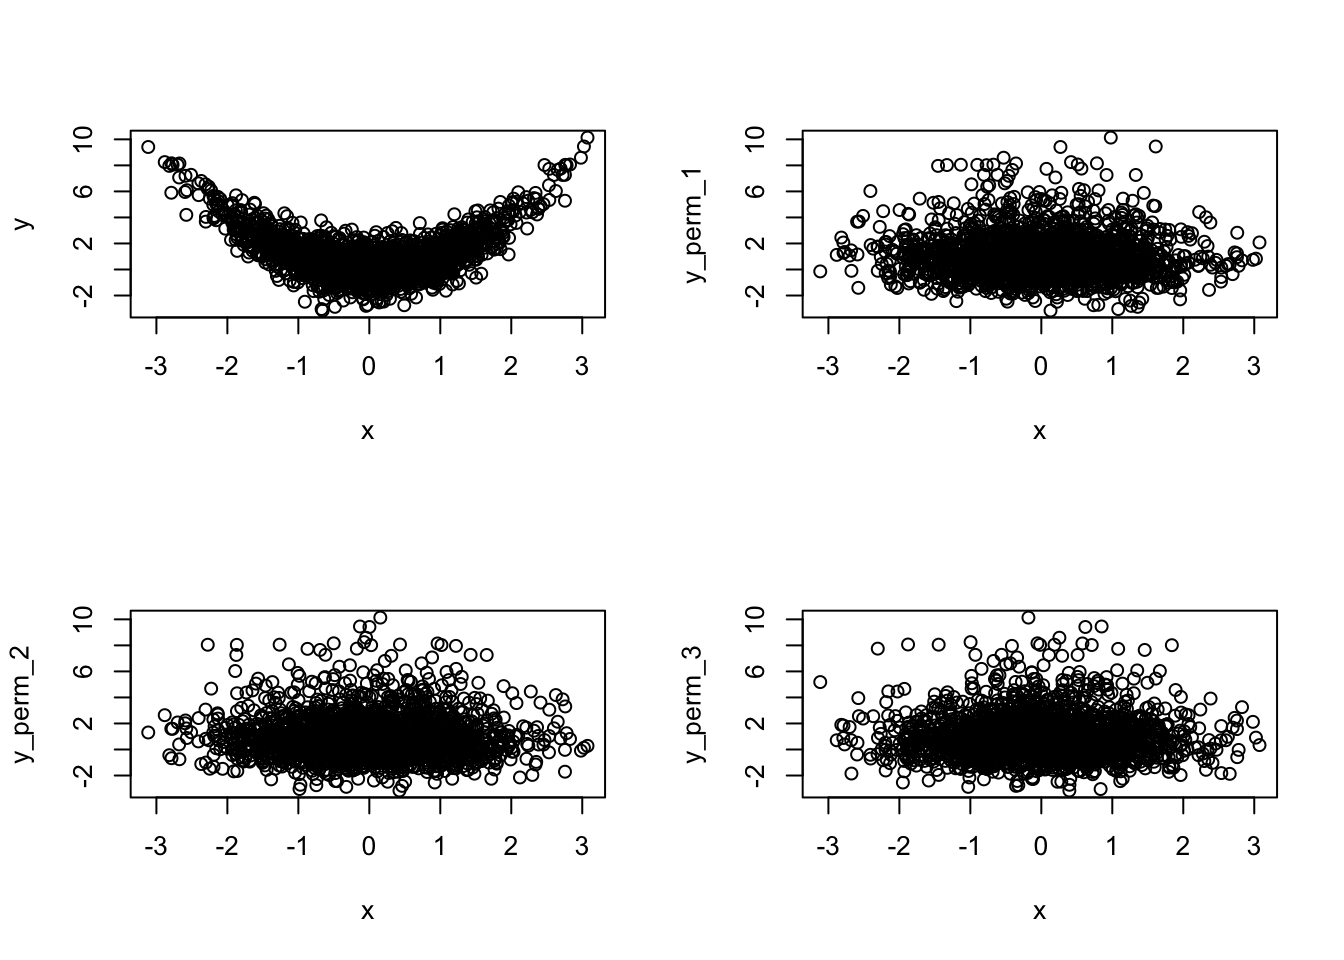
\includegraphics{_main_files/figure-latex/unnamed-chunk-75-1} \end{center}

\begin{enumerate}
\def\labelenumi{\arabic{enumi}.}
\setcounter{enumi}{1}
\tightlist
\item
\end{enumerate}

\begin{Shaded}
\begin{Highlighting}[]
\FunctionTok{hist}\NormalTok{(x)}
\FunctionTok{hist}\NormalTok{(y)}
\end{Highlighting}
\end{Shaded}

\begin{center}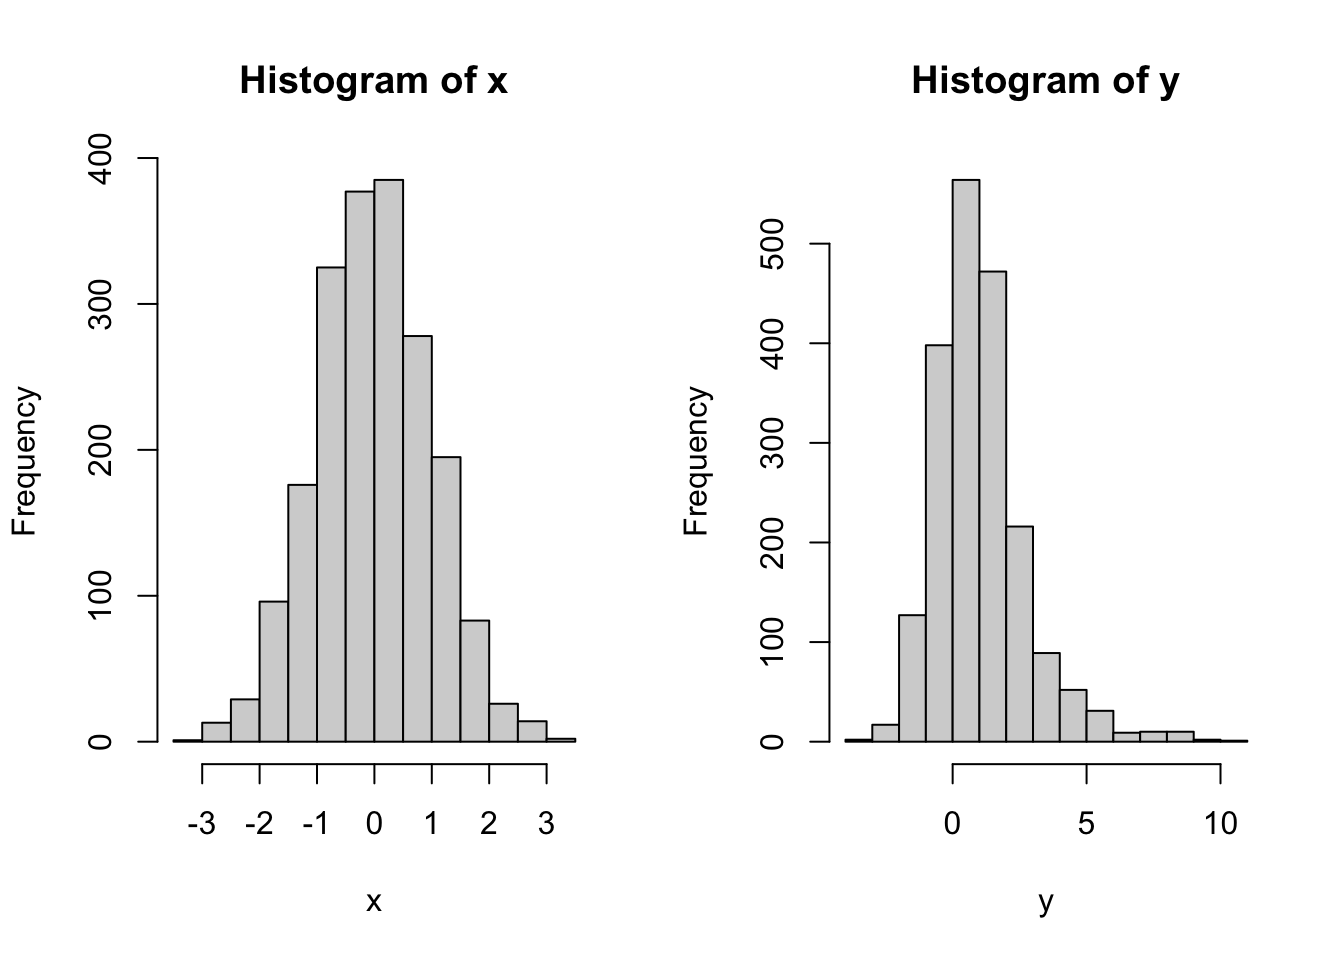
\includegraphics{_main_files/figure-latex/unnamed-chunk-76-1} \end{center}

No, the two histograms would not be enough to describe the joint distribution.
There are many ways in which two random variables \(X\) and \(Y\) can be jointly
distributed, but whose separate (marginal) distributions match the histograms
above. To give a very simple example, let \(X\) and \(Y\) be discrete random
variables, each of which can only take values \(0\) or \(1\). Consider the following
two possible \emph{joint} distribution tables for the random pair \((X,Y)\):

0

1

0

0.25

0.25

1

0.25

0.25

0

1

0

0.5

0.0

1

0.0

0.5

In both cases, the marginals are the same, i.e., both \(X\) and \(Y\) are equally
likely to take the value \(0\) or \(1\), i.e., they both have the Bernoulli
distribution with parameter \(p=1/2\). That would correspond to the separate
histograms to be the same. On the other hand, their joint distributions (aka
dependence structures) are completely different. In the first (left) case, \(X\)
and \(Y\) are independent, but in the second they are completely dependent.

\begin{enumerate}
\def\labelenumi{\arabic{enumi}.}
\setcounter{enumi}{2}
\tightlist
\item
\end{enumerate}

They are probably not correlated since the sample correlation between \texttt{x}
and \texttt{y} is close to \(0\):

\begin{Shaded}
\begin{Highlighting}[]
\NormalTok{(}\FunctionTok{cor}\NormalTok{(x, y))}
\DocumentationTok{\#\# [1] {-}0.02880239}
\end{Highlighting}
\end{Shaded}

but they do not look independent.

To apply the permutation test, we first plot the scatterplot of \texttt{x} vs.~\texttt{y} as
above. Then, we replace \texttt{y} by a vector with the same components, but randomly
permute their positions, and then plot a scatterplot again. We repeat this three
times:

\begin{Shaded}
\begin{Highlighting}[]
\NormalTok{y\_perm\_1 }\OtherTok{=} \FunctionTok{sample}\NormalTok{(y)}
\NormalTok{y\_perm\_2 }\OtherTok{=} \FunctionTok{sample}\NormalTok{(y)}
\NormalTok{y\_perm\_3 }\OtherTok{=} \FunctionTok{sample}\NormalTok{(y)}
\FunctionTok{plot}\NormalTok{(x, y)}
\FunctionTok{plot}\NormalTok{(x, y\_perm\_1)}
\FunctionTok{plot}\NormalTok{(x, y\_perm\_2)}
\FunctionTok{plot}\NormalTok{(x, y\_perm\_3)}
\end{Highlighting}
\end{Shaded}

\begin{center}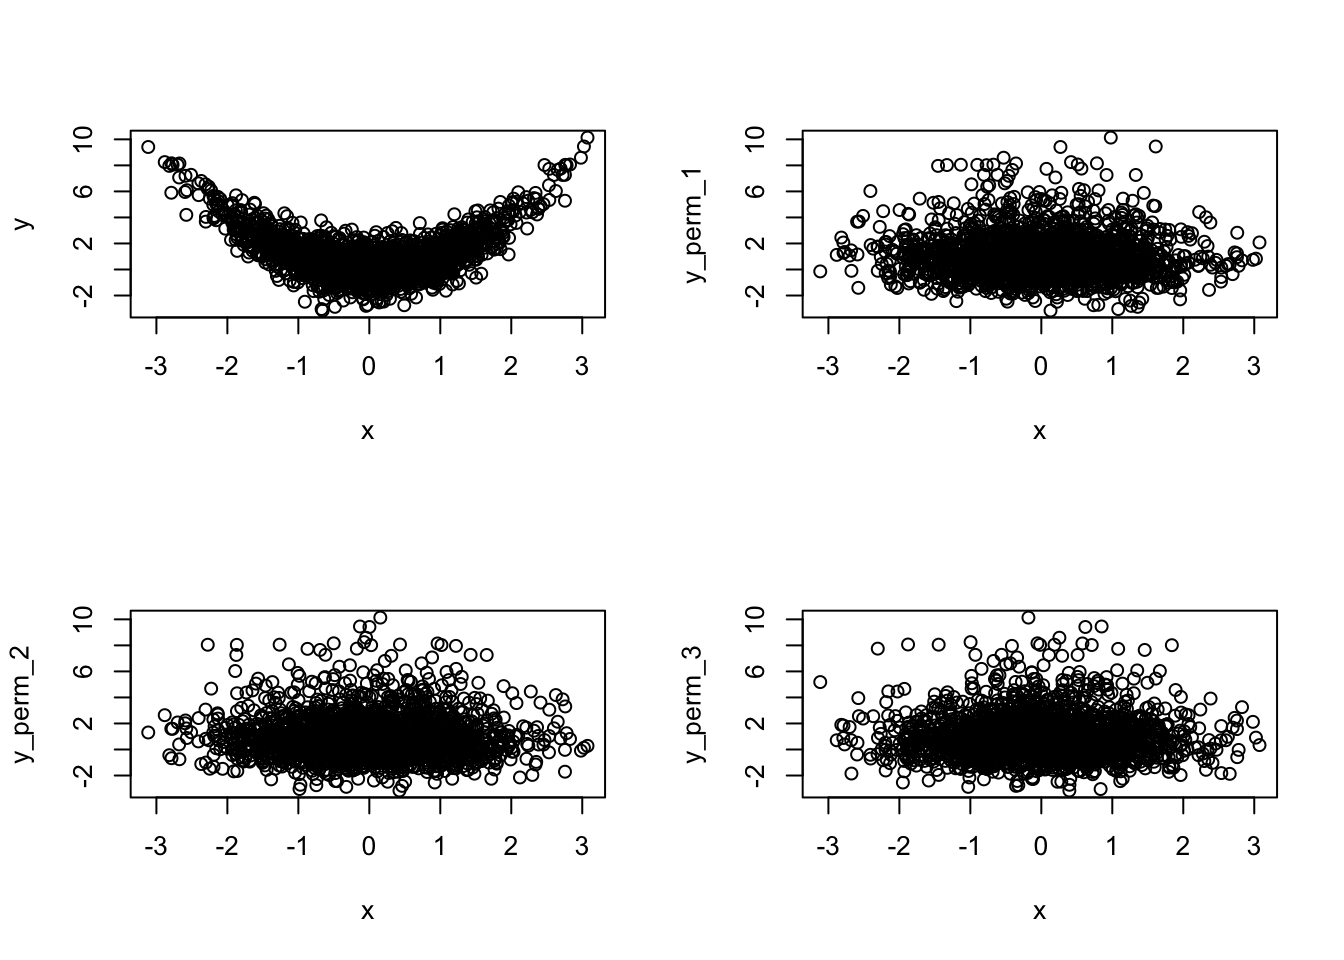
\includegraphics{_main_files/figure-latex/unnamed-chunk-79-1} \end{center}

The conclusion is clear, the first (upper-left) plot is very different than the
other three. Therefore, \texttt{x} and \texttt{y} are probably not independent.

\emph{Comments (Math):} The point of this problem is to review the notion of the \textbf{joint
distribution} between two random variables. The most important point here is
that there is more to the joint distribution of two random vectors, than just
the two distributions taken separately. In a sense, the whole is (much) more
than the sum of its parts. This is something that does not happen in the
deterministic world. If you give me the \(x\)-coordinate of a point, and,
separately, its \(y\)-coordinate, I will be able to pinpoint the exact location of
that point.

On the other hand, suppose that the \(x\)-coordinate of a point is unknown, so we
treat it as a random variable, and suppose that this variable admits the
standard normal distribution. Do the same for \(y\). Even with this information,
you cannot say anything about the position of the point \((x,y)\). It could be
that the reason we are uncertain about \(x\) and the reason we are uncertain about
\(y\) have nothing to do with each other; in that case we would be right to assume
that \(x\) and \(y\) are independent. If, on the other hand, we got the values of
both \(x\) and \(y\) by measuring them using the same, inaccurate, tape measure, we
cannot assume that the errors are independent. It is more likely that both \(x\)
and \(y\) are too big, or both \(x\) and \(y\) are too small.

Mathematically, we say that random variables \(X\) and \(Y\) are independent if
\[{\mathbb{P}}[X \in [a,b]] \times {\mathbb{P}}[ Y \in [c,d] ] = {\mathbb{P}}[ X\in [a,b] \text{ and } Y\in [c,d]]\text{ for all } a,b,c,d.\]
While up to the point,
this definition is not very eye-opening, or directly applicable in most cases.
Intuitively, \(X\) and \(Y\) are independent if the distribution of \(Y\) would not
change if we received additional information about \(X\). In our problem, random
variables \(X\) and \(Y\) correspond to vectors \texttt{x} and \texttt{y}. Their scatterplot above
clearly conveys the following message: when \texttt{x} is around \(-2\), we expect \texttt{y} to
be around \texttt{4}, while when \texttt{x} is around \(0\), \texttt{y} would be expected to be around
\(0\), too.

Sometimes, it is not so easy to decide whether two variables are independent by staring at a scatterplot. What would you say about the scatterplot below?

\begin{center}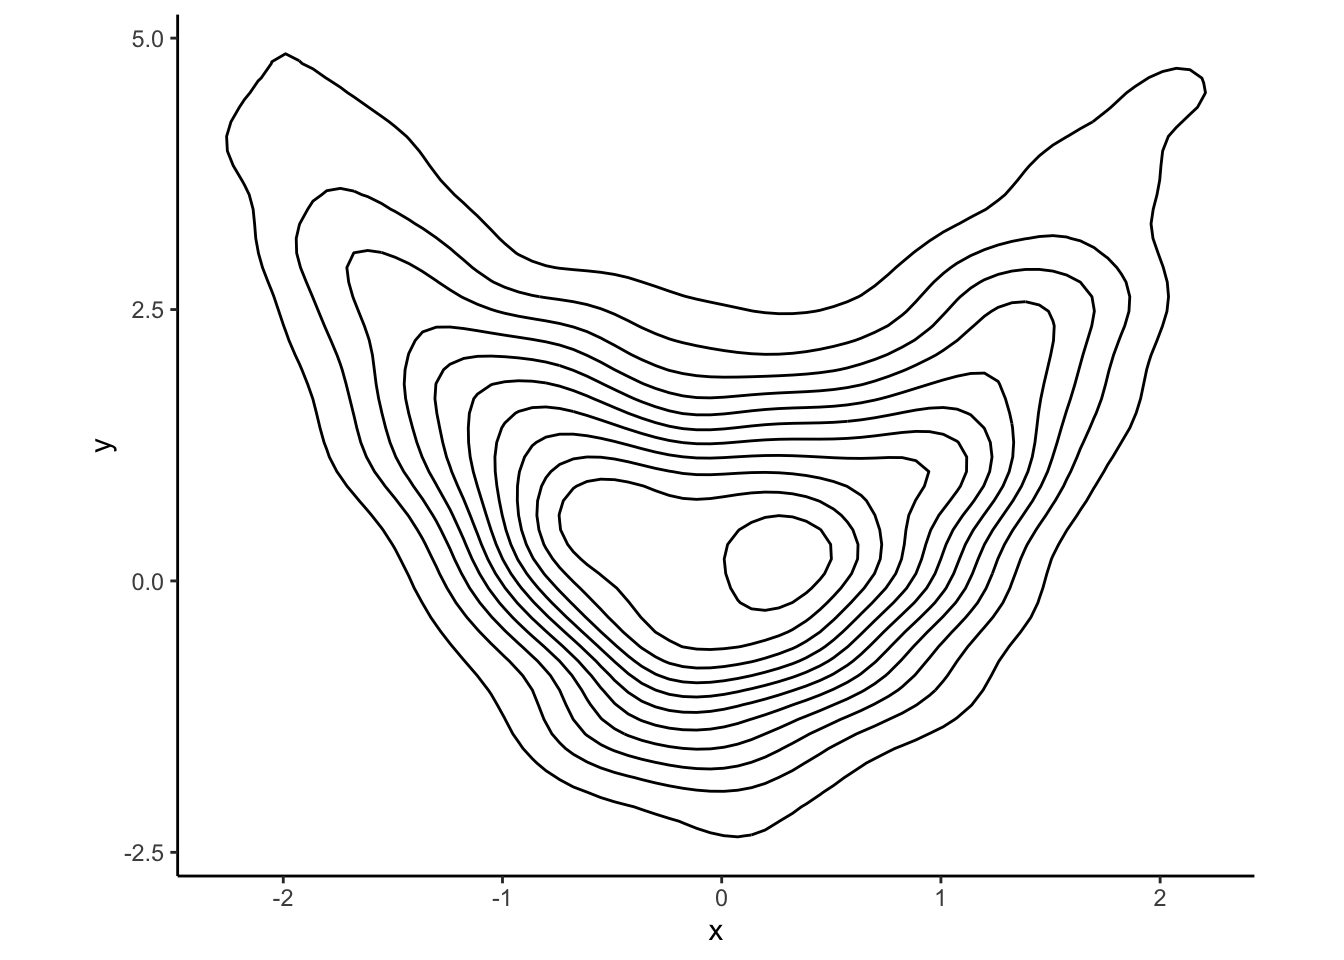
\includegraphics[width=0.5\linewidth]{_main_files/figure-latex/unnamed-chunk-80-1} \end{center}

The \textbf{permutation test} is designed to help you decide when two (simulated)
random variables are likely to be independent. The idea is simple. Suppose that
\texttt{x} and \texttt{y} are simulations from two independent (not necessarily identical)
distributions; say \texttt{x=runif(1000)} and \texttt{y=rnorm(1000)}. The vector
\texttt{y\_perm=sample(y)} is a randomly permuted version of \texttt{y} (see R section below)
and it contains exactly the same information about the distribution of \texttt{y} as
\texttt{y} itself does. Both \texttt{y} and \texttt{y\_perm} will produce exactly the same histogram.
Permuting \texttt{y}, however, ``uncouples'' it from \texttt{x}. If there was any dependence
between the values of \texttt{x} and \texttt{y} before, there certainly isn't any now. In
other the joint distribution of \texttt{x} and \texttt{y\_perm} has the same marginals as the
joint distribution of \texttt{x} and \texttt{y}, but all the (possible) dependence has been
removed. What remains is to compare the scatterplot between \texttt{x} and \texttt{y} and the
scatterplot between \texttt{x} and \texttt{y\_perm}. If they look about the same, we conclude
that \texttt{x} and \texttt{y} are independent. Otherwise, there is some dependence between
them.

One question remains: why did we have to draw three scatterplots of permuted
versions of \texttt{y}? That is because we have only finitely many data points, and it
can happen, by pure chance, that the permutation we applied to \texttt{y} does not
completely scramble its dependence on \texttt{x}. With a ``sample'' of three such plots,
we
get a better feeling for the inherent randomness in this permutation procedure,
and it is much easier to tell whether ``one of these things is not like the
others''. Btw, the random variables in the scatterplot above are, indeed,
independent; here are the \(4\) permutation-test plots to ``prove'' it:

\begin{center}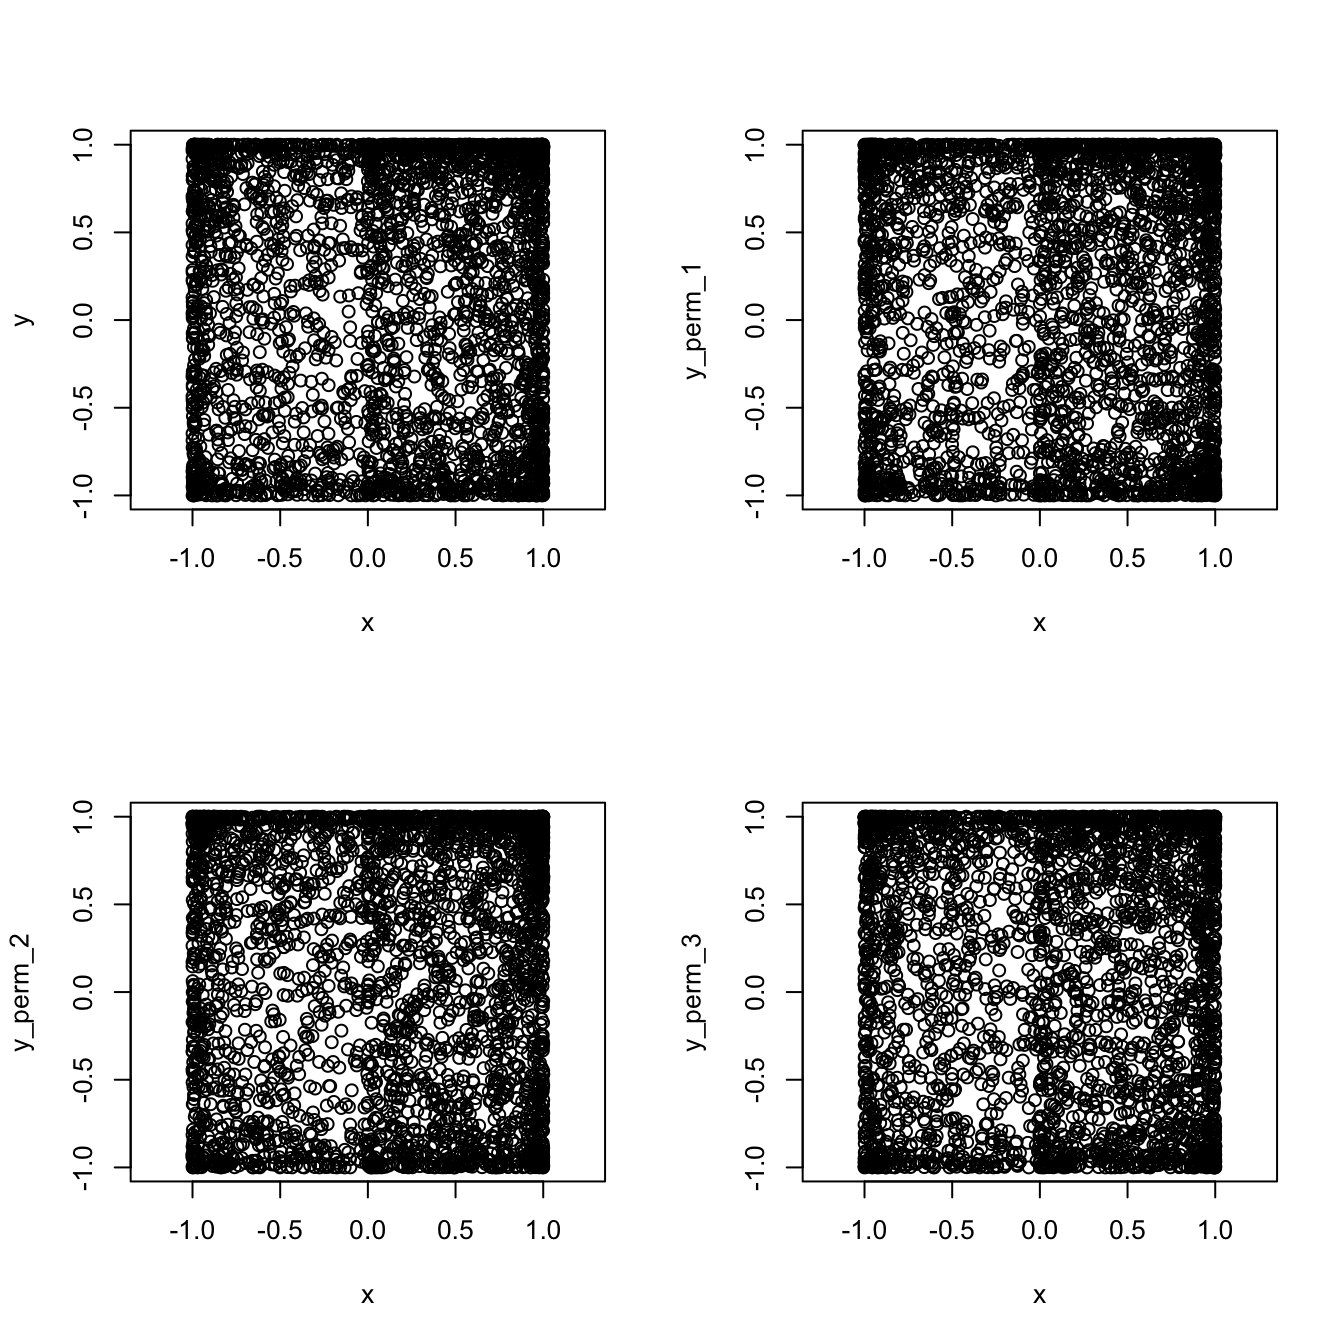
\includegraphics{_main_files/figure-latex/unnamed-chunk-81-1} \end{center}

Unlike univariate (one-variable) distributions which are visualized using
histograms or similar plots, multivariate (several-variable) distributions are
harder to depict. The most direct relative of the histogram is a \textbf{3d
histogram}. Just like the \(x\)-axis is divided into bins in the univariate case,
in the multivariate case we divide the \(xy\)-plane into regions (squares, e.g.)
and count the number of points falling into each of these regions. After that
a 3d bar (a skyscraper) is drawn above each square with the height of each
skyscraper equal (or proportional) to the number of points which fall into its
base. Here is a 3d histogram of our original pair (\texttt{x},\texttt{y}) from the problem.
You should be able to rotate and zoom it right here in the notes, provided your
browser has JavaScript enabled:

A visualization solution that requires less technology would start the same way,
i.e., by dividing the \(xy\) plane into regions, but instead of the third
dimension, it would use different colors to represent the counts. Here is an
example where the regions are hexagons, as opposed to squares; it just looks
better, for some reason:

\begin{center}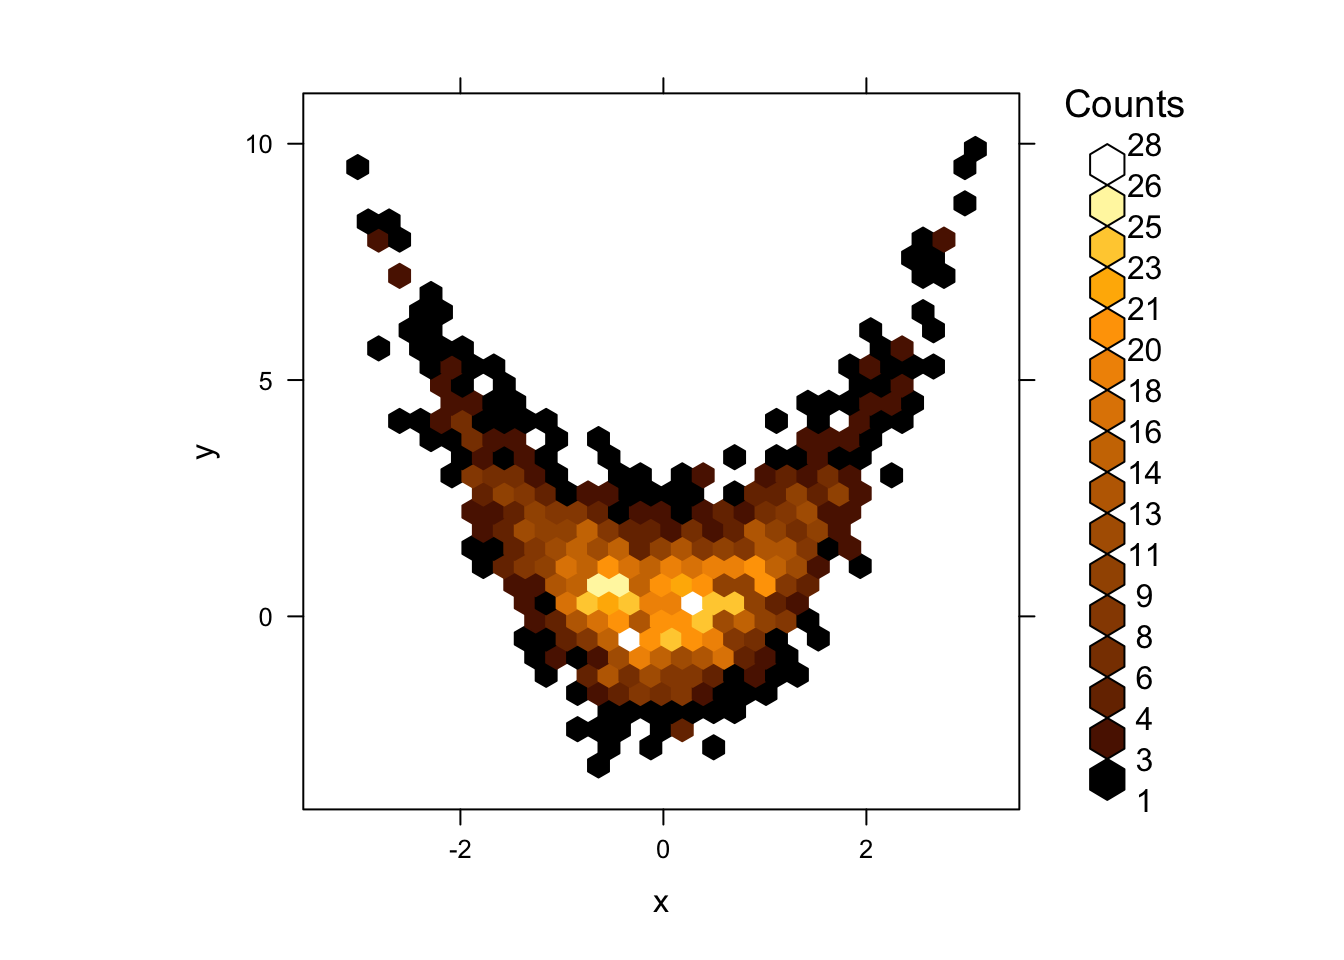
\includegraphics{_main_files/figure-latex/unnamed-chunk-83-1} \end{center}

Just to showcase the range of possibilities, here is another visualization
technique which which requires deeper statistical tools, namely the
\textbf{density contour plot}:

\begin{center}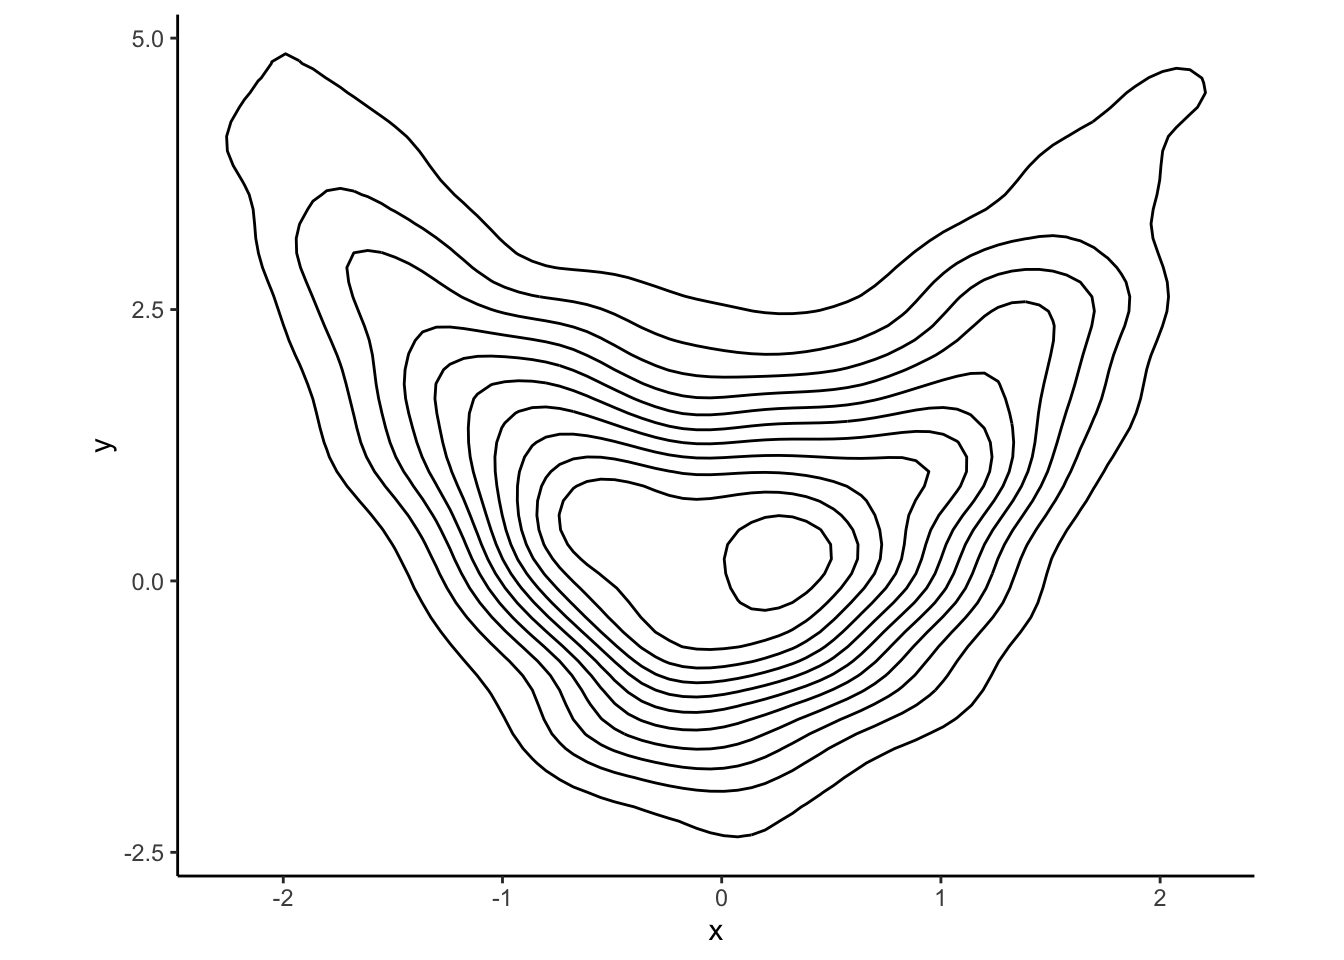
\includegraphics[width=0.8\linewidth]{_main_files/figure-latex/unnamed-chunk-84-1} \end{center}

\emph{Comments (R):} There is very little new R here. You should remember that if \texttt{x} and \texttt{y} are
vectors of the same length, \texttt{plot(x,y)} gives you a scatterplot of \texttt{x} and \texttt{y}.

To compute the sample correlation between two vectors, use the \texttt{cor}.

We used the command \texttt{sample(y)} to obtain a randomly permuted version of \texttt{y}.
The simplicity of this is due to default parameters of the command \texttt{sample}
which we already learned about. In particular, the default number of samples is
exactly the size of the input vector \texttt{y} and, by default, sampling is performed
\emph{without replacement}. If you think about it for a second, you will realize that
a sample of size \(n\) from the vector of size \(n\) \emph{without} replacement is
nothing by a random permutation of \texttt{y}.

You are not required to do this in your submissions, but if you want to display
several plots side-by-side, use the command \texttt{par(mfrow=c(m,n))} before the command
\texttt{plot}. It tells R to plot the next \(mn\) plots in a \(m\times n\) grid.
\end{solution}

\begin{exercise}
Let the random variables \(X\) and \(Y\) have the joint distribution given by
the following table:

1

2

3

1

0.1

0.2

0.3

2

0.2

0.2

0.0

Simulate \(10,000\) draws from the distribution of \((X,Y)\) and display a
contingency table of your results.
\end{exercise}

\begin{solution}
~

\begin{Shaded}
\begin{Highlighting}[]
\NormalTok{joint\_distribution\_long }\OtherTok{=} \FunctionTok{data.frame}\NormalTok{(}
   \AttributeTok{x =} \FunctionTok{c}\NormalTok{(}\DecValTok{1}\NormalTok{, }\DecValTok{1}\NormalTok{, }\DecValTok{1}\NormalTok{, }\DecValTok{2}\NormalTok{, }\DecValTok{2}\NormalTok{, }\DecValTok{2}\NormalTok{),}
   \AttributeTok{y =} \FunctionTok{c}\NormalTok{(}\DecValTok{1}\NormalTok{, }\DecValTok{2}\NormalTok{, }\DecValTok{3}\NormalTok{, }\DecValTok{1}\NormalTok{, }\DecValTok{2}\NormalTok{, }\DecValTok{3}\NormalTok{)}
\NormalTok{)}
\NormalTok{probabilities\_long }\OtherTok{=} 
       \FunctionTok{c}\NormalTok{(}\FloatTok{0.1}\NormalTok{, }\FloatTok{0.2}\NormalTok{, }\FloatTok{0.3}\NormalTok{, }\FloatTok{0.2}\NormalTok{, }\FloatTok{0.2}\NormalTok{, }\FloatTok{0.0}\NormalTok{)}

\NormalTok{sampled\_rows }\OtherTok{=} \FunctionTok{sample}\NormalTok{(}
   \AttributeTok{x =} \DecValTok{1}\SpecialCharTok{:}\FunctionTok{nrow}\NormalTok{(joint\_distribution\_long),}
   \AttributeTok{size =} \DecValTok{10000}\NormalTok{,}
   \AttributeTok{replace =} \ConstantTok{TRUE}\NormalTok{,}
   \AttributeTok{prob =}\NormalTok{ probabilities\_long}
\NormalTok{)}

\NormalTok{draws }\OtherTok{=}\NormalTok{ joint\_distribution\_long[sampled\_rows, ]}

\FunctionTok{table}\NormalTok{(draws)}
\DocumentationTok{\#\#    y}
\DocumentationTok{\#\# x      1    2    3}
\DocumentationTok{\#\#   1  962 2027 3047}
\DocumentationTok{\#\#   2 1945 2019    0}
\end{Highlighting}
\end{Shaded}

\emph{Comments (Math):} The main mathematical idea is to think of \emph{each pair} of possible values
of \(X\) and \(Y\) as a separate ``object'', put all these objects in a ``bag'', then
then draw from the bag. In other words, we convert the bivariate distribution
from the problem to the following univariate distribution

(1,1)

(1,2)

(1,3)

(2,1)

(2,2)

(2,3)

0.1

0.2

0.3

0.2

0.2

0

and sample from it. When you do, you will get a vector whose elements are pairs
of numbers. The last step is to extract the components of those pairs into
separate vectors.

\emph{Comments (R):} The most important new R concept here is \texttt{data.frame}. You should think of
it as a spreadsheet. It is, mathematically, a matrix, but we do not perform any
mathematical operations on it. Moreover, not all columns in the data frame have
to be numeric. Some of them can be strings, and other can be something even more
exotic. You should think of a data frame as a bunch of column vectors of the
same length stacked side by side. It is important to note that each column of a
data frame will have a name, so that we don't have to access it by its position
only (as we would have to in the case of a matrix).

In this class, the column vectors of data frames are going to contain simulated
values. In statistics, it is data that comes in data frames, with rows
corresponding to different observations, and columns to various observed
variables.

The easiest way to construct a data frame using already existing vectors is as follows:

\begin{Shaded}
\begin{Highlighting}[]
\NormalTok{x }\OtherTok{=} \FunctionTok{c}\NormalTok{(}\DecValTok{1}\NormalTok{, }\DecValTok{2}\NormalTok{, }\DecValTok{3}\NormalTok{)}
\NormalTok{y }\OtherTok{=} \FunctionTok{c}\NormalTok{(}\StringTok{"a"}\NormalTok{, }\StringTok{"b"}\NormalTok{, }\StringTok{"c"}\NormalTok{)}
\NormalTok{(}\AttributeTok{df =} \FunctionTok{data.frame}\NormalTok{(x, y))}
\DocumentationTok{\#\#   x y}
\DocumentationTok{\#\# 1 1 a}
\DocumentationTok{\#\# 2 2 b}
\DocumentationTok{\#\# 3 3 c}
\end{Highlighting}
\end{Shaded}

Note that the two columns inherited their names from the vectors \texttt{x} and \texttt{y}
that fed into them. Note, also, that all rows got consecutive numerical values
as names by default. Row names are sometimes useful to have, but are in general
a nuisance and should be ignored (especially in this class). Column names are
more important, and there is a special notation (the dollar-sign notation) that
allows you to access a column by its name:

\begin{Shaded}
\begin{Highlighting}[]
\NormalTok{df}\SpecialCharTok{$}\NormalTok{y}
\DocumentationTok{\#\# [1] "a" "b" "c"}
\end{Highlighting}
\end{Shaded}

If you want to give your columns custom names (or if you are building them out
of explicitly given vectors as in the solution above) use the following syntax

\begin{Shaded}
\begin{Highlighting}[]
\NormalTok{z }\OtherTok{=} \FunctionTok{c}\NormalTok{(}\StringTok{"a"}\NormalTok{, }\StringTok{"b"}\NormalTok{, }\StringTok{"c"}\NormalTok{, }\StringTok{"d"}\NormalTok{)}
\NormalTok{(}\AttributeTok{df =} \FunctionTok{data.frame}\NormalTok{(}\AttributeTok{letters =}\NormalTok{ z, }\AttributeTok{numbers =} \FunctionTok{c}\NormalTok{(}\DecValTok{1}\NormalTok{, }\DecValTok{2}\NormalTok{, }\DecValTok{3}\NormalTok{, }\DecValTok{4}\NormalTok{)))}
\DocumentationTok{\#\#   letters numbers}
\DocumentationTok{\#\# 1       a       1}
\DocumentationTok{\#\# 2       b       2}
\DocumentationTok{\#\# 3       c       3}
\DocumentationTok{\#\# 4       d       4}
\end{Highlighting}
\end{Shaded}

A feature that data frames share with vectors and matrices is that you can use vector indexing as in the following example (where \texttt{df} is as above)

\begin{Shaded}
\begin{Highlighting}[]
\NormalTok{df[}\FunctionTok{c}\NormalTok{(}\DecValTok{2}\NormalTok{, }\DecValTok{4}\NormalTok{, }\DecValTok{4}\NormalTok{, }\DecValTok{1}\NormalTok{), ]}
\DocumentationTok{\#\#     letters numbers}
\DocumentationTok{\#\# 2         b       2}
\DocumentationTok{\#\# 4         d       4}
\DocumentationTok{\#\# 4.1       d       4}
\DocumentationTok{\#\# 1         a       1}
\end{Highlighting}
\end{Shaded}

Make sure you understand why the expression inside the brackets is \texttt{c(2,4,4,1),}
and not \texttt{c(2,4,4,1)}. R's desire to keep row names unique leads to some
cumbersome constructs such as \texttt{4.1} above. As I mentioned before, just disregard
them.

A nice thing about data frames is that they can easily be pretty-printed in
RStudio. Go to the Environment tab in one of your RStudio panes, and double
click on the name of the data frame you just built. It will appear as a nicely
formatted spreadsheet.

Once we have the data frame containing all \(6\) pairs of possible values \(X\) and
\(Y\) can take (called \texttt{joint\_distribution\_long} in the solution above), we can
proceed by sampling from its rows, by sampling from the set \texttt{1,2,3,4,5,6} with
probabilities \texttt{0.1,\ 0.2,\ 0.3,\ 0.2,\ 0.2,\ 0.0}. The result of the corresponding
\texttt{sample} command will be a sequence - called \texttt{sampled\_rows} in the solution - of
length \(10,000\) composed of numbers \(1,2,3,4,5\) or \(6\). The reason we chose the
name \texttt{sampled\_rows} is because each number corresponds to a row from the data
frame \texttt{joint\_distribution\_long}, and by indexing \texttt{joint\_distribution\_long} by
\texttt{sampled\_rows} we are effectively sampling from its rows. In other words, the
command \texttt{joint\_distribution\_long{[}sampled\_rows,\ {]}} turns a bunch of numbers into
a bunch of rows (many of them repeated) of the data frame
\texttt{joint\_distribution\_long}.

The final step is to use the function \texttt{table}. This time, we are applying it to
a data frame and not to a vector, but the effect is the same. It tabulates all
possible combinations of values of the columns, and counts how many times each
of them happened. The same result would have been obtained by calling
\texttt{table(draws\$x,\ draws\$y)}.
\end{solution}

\hypertarget{monte-carlo}{%
\section{Monte Carlo}\label{monte-carlo}}

\begin{exercise}
Use Monte Carlo to estimate the expected value of the exponential random
variable with parameter \(\lambda= 4\) using \(n=10\), \(n=1,000\) and \(n=1,000,000\)
simulations. Compare to the exact value.
\end{exercise}

\begin{solution}
~

\begin{Shaded}
\begin{Highlighting}[]
\NormalTok{x }\OtherTok{=} \FunctionTok{rexp}\NormalTok{(}\DecValTok{10}\NormalTok{, }\AttributeTok{rate =} \DecValTok{4}\NormalTok{)}
\FunctionTok{mean}\NormalTok{(x)}
\DocumentationTok{\#\# [1] 0.1779768}
\end{Highlighting}
\end{Shaded}

For an exponential random variable with parameter \(\lambda\), the expected value is
\(1/\lambda\) (such information can be found in \href{./dist.html}{Appendix A}) which,
in this case, is \(0.25\). The error made was 0.072023 for \(n=10\) simulations.

We increase the number of simulations to \(n=1000\) and get a better result

\begin{Shaded}
\begin{Highlighting}[]
\NormalTok{x }\OtherTok{=} \FunctionTok{rexp}\NormalTok{(}\DecValTok{1000}\NormalTok{, }\AttributeTok{rate =} \DecValTok{4}\NormalTok{)}
\FunctionTok{mean}\NormalTok{(x)}
\DocumentationTok{\#\# [1] 0.2564643}
\end{Highlighting}
\end{Shaded}

with (smaller) error -0.0064643. Finally, let's try \(n=1,000,000\):

\begin{Shaded}
\begin{Highlighting}[]
\NormalTok{x }\OtherTok{=} \FunctionTok{rexp}\NormalTok{(}\FloatTok{1e+06}\NormalTok{, }\AttributeTok{rate =} \DecValTok{4}\NormalTok{)}
\FunctionTok{mean}\NormalTok{(x)}
\DocumentationTok{\#\# [1] 0.250381}
\end{Highlighting}
\end{Shaded}

The error is even smaller -0.00038101.

\emph{Comments (R):} The only new thing here is the command \texttt{mean} which computes the mean of a vector.

\emph{Comments (Math):} There is a lot going on here conceptually. This is the first time we
used the Monte Carlo method. It is an incredibly useful tool, as you will keep
being reminded throughout this class. The idea behind it is simple, and it is
based on the \emph{Law of large numbers}:

\textbf{Theorem} Let \(X_1,X_2, \dots\) be an independent sequence of random
variables with the same distribution, for which the expected value can be
computed. Then
\[ \tfrac{1}{n} \Big( X_1+X_2+\dots+X_n\Big) \to {\mathbb{E}}[X_1] \text{ as } n\to\infty\]
The idea behind Monte Carlo is to turn this theorem ``upside down''. The goal is
to compute \({\mathbb{E}}[X_1]\) and use a supply of random numbers, each of which
comes from the same distribution, to accomplish that. The random number
generator inside \texttt{rexp} gives us a supply of numbers (stored in the vector \texttt{x})
and all we have to do is compute their average. This gives us the left-hand side
of the formula above, and, if \(n\) is large enough, we hope that this average
does not differ too much from its theoretical limit. As \(n\) gets larger, we
expect better and better results. That is why your error above gets smaller as
\(n\) increases.

It looks like Monte Carlo can only be used to compute the expected value of a
random variable, which does not seem like such a bit deal. But it is! You will see
in the sequel that almost anything can be written as the expected value of
\emph{some} random variable.
\end{solution}

\begin{exercise}
Use Monte Carlo to estimate \({\mathbb{E}}[X^2]\), where \(X\) is a standard normal
random variable.
\end{exercise}

\begin{solution}
You may or may now know that when \(X\) is standard normal \(Y=X^2\) has a \(\chi^2\)
distribution with one degree of freedom. If you do, you can solve the problem
like this:

\begin{Shaded}
\begin{Highlighting}[]
\NormalTok{y }\OtherTok{=} \FunctionTok{rchisq}\NormalTok{(}\DecValTok{5000}\NormalTok{, }\AttributeTok{df =} \DecValTok{1}\NormalTok{)}
\FunctionTok{mean}\NormalTok{(y)}
\DocumentationTok{\#\# [1] 0.9771929}
\end{Highlighting}
\end{Shaded}

If you don't, you can do the following:

\begin{Shaded}
\begin{Highlighting}[]
\NormalTok{x }\OtherTok{=} \FunctionTok{rnorm}\NormalTok{(}\DecValTok{5000}\NormalTok{)}
\NormalTok{y }\OtherTok{=}\NormalTok{ x}\SpecialCharTok{\^{}}\DecValTok{2}
\FunctionTok{mean}\NormalTok{(y)}
\DocumentationTok{\#\# [1] 1.019852}
\end{Highlighting}
\end{Shaded}

\emph{Comments (Math+R):} We are asked to compute \({\mathbb{E}}[ X^2]\), which can be interpreted in
two ways. First, we can think of \(Y=X^2\) as a random variable in its own right and you
can try to take draws from the distribution of \(Y\). In the case of the normal
distribution, the distribution of \(Y\) is known - it happens to be a
\(\chi^2\)-distribution with a single degree of freedom (don't worry if you never
heard of it). We can simulate it in R by using its R name \texttt{chisq} and
get a number close to the exact value of \(1\).

If you did not know about the \(\chi^2\) distribution, you would not know what R
name to put the prefix \texttt{r} in front of. What makes the simulation possible is
the fact that \(Y\) is a \emph{transformation} of
a random variable we know how to simulate. In that case, we simply simulate the
required number of draws \texttt{x} from the geometric distribution (using \texttt{rnorm}) and
then apply the transformation \(x \mapsto x^2\) to the result. The transformed
vector \texttt{y} is then nothing but the sequence of draws from the distribution of
\(X^2\).

The idea described above is one of main advantages of the Monte Carlo technique:
if you know how to simulate a random variable, you also know how to simulate
any (deterministic) function of it. That fact will come into its own a bit later
when we start working with several random variables and stochastic processes,
but it can be very helpful even in the case of a single random variable, as you
will see in the next problem.
\end{solution}

\begin{exercise}
Let \(X\) be a standard normal random variable. Use Monte Carlo to estimate the
probability \({\mathbb{P}}[ X > 1 ]\). Compare to the exact value.
\end{exercise}

\begin{solution}
The estimated probability:

\begin{Shaded}
\begin{Highlighting}[]
\NormalTok{x }\OtherTok{=} \FunctionTok{rnorm}\NormalTok{(}\DecValTok{10000}\NormalTok{)}
\NormalTok{y }\OtherTok{=}\NormalTok{ x }\SpecialCharTok{\textgreater{}} \DecValTok{1}
\NormalTok{(}\AttributeTok{p\_est =} \FunctionTok{mean}\NormalTok{(y))}
\DocumentationTok{\#\# [1] 0.1608}
\end{Highlighting}
\end{Shaded}

The exact probability and the error

\begin{Shaded}
\begin{Highlighting}[]
\NormalTok{p\_true }\OtherTok{=} \DecValTok{1} \SpecialCharTok{{-}} \FunctionTok{pnorm}\NormalTok{(}\DecValTok{1}\NormalTok{)}
\NormalTok{(}\AttributeTok{err =}\NormalTok{ p\_est }\SpecialCharTok{{-}}\NormalTok{ p\_true)}
\DocumentationTok{\#\# [1] 0.002144746}
\end{Highlighting}
\end{Shaded}

\emph{Comments (R):} As we learned before, the symbol \texttt{\textgreater{}} is an operation, which returns a Boolean (\texttt{TRUE} or \texttt{FALSE}) value. For example:

\begin{Shaded}
\begin{Highlighting}[]
\DecValTok{1} \SpecialCharTok{\textgreater{}} \DecValTok{2}
\DocumentationTok{\#\# [1] FALSE}
\end{Highlighting}
\end{Shaded}

\begin{Shaded}
\begin{Highlighting}[]
\DecValTok{5}\SpecialCharTok{\^{}}\DecValTok{2} \SpecialCharTok{\textgreater{}} \DecValTok{20}
\DocumentationTok{\#\# [1] TRUE}
\end{Highlighting}
\end{Shaded}

It is vectorized:

\begin{Shaded}
\begin{Highlighting}[]
\NormalTok{x }\OtherTok{=} \FunctionTok{c}\NormalTok{(}\DecValTok{1}\NormalTok{, }\DecValTok{2}\NormalTok{, }\DecValTok{4}\NormalTok{)}
\NormalTok{y }\OtherTok{=} \FunctionTok{c}\NormalTok{(}\DecValTok{5}\NormalTok{, }\SpecialCharTok{{-}}\DecValTok{4}\NormalTok{, }\DecValTok{3}\NormalTok{)}
\NormalTok{x }\SpecialCharTok{\textgreater{}}\NormalTok{ y}
\DocumentationTok{\#\# [1] FALSE  TRUE  TRUE}
\end{Highlighting}
\end{Shaded}

and recycling rules apply to it (so that you can compare a vector and a scalar, for example)

\begin{Shaded}
\begin{Highlighting}[]
\NormalTok{x }\OtherTok{=} \DecValTok{1}\SpecialCharTok{:}\DecValTok{10}
\NormalTok{x }\SpecialCharTok{\textgreater{}} \DecValTok{5}
\DocumentationTok{\#\#  [1] FALSE FALSE FALSE FALSE FALSE  TRUE  TRUE  TRUE  TRUE  TRUE}
\end{Highlighting}
\end{Shaded}

Therefore, the vector \texttt{y} in the solution is a vector of length \(10000\) whose
elements are either \texttt{TRUE} or \texttt{FALSE}; here are the first 5 rows of data frame
with columns \texttt{x} and \texttt{y} from our solution:

x

y

1.9493

FALSE

-1.1015

TRUE

1.0448

TRUE

-0.1384

TRUE

-0.2573

TRUE

Finally, \texttt{z} contains the \texttt{mean} of \texttt{y}. How do you compute a mean of Boolean values? In R (and many other languages) \texttt{TRUE} and \texttt{FALSE} have default numerical values, usually \(1\) and \(0\). This way, when \(R\) is asked to compute the \texttt{sum} of a Boolean vector it will effectively count the number of values which are \texttt{TRUE}. Similarly, the \texttt{mean} is the relative proportion of \texttt{TRUE} values.

\emph{Comments (Math):} We computed the \textbf{proportion} of the ``times'' \(X>1\) (among many simulations of \(X\)) and used it to approximate the \textbf{probability} \({\mathbb{P}}[ X>1]\). More formally,
we started from a random variable \(X\) with a normal distribution and then transformed it into another random variable, \(Y\), by setting \(Y=1\) whenever \(X>1\) and \(0\) otherwise. This is often written as follows
\[ Y = \begin{cases} 1, & X>1 \\ 0, & X\leq 1.\end{cases}\]
The random variable \(Y\) is very special - it can only take values \(0\) and \(1\) (i.e., its support is \(\{0,1\}\)). Such random variables are called \textbf{indicator random variables}, and their distribution, called the \textbf{Bernoulli distribution}, always looks like this:

0

1

1-p

p

for some \(p \in [0,1]\). The parameter \(p\) is nothing but the probability \({\mathbb{P}}[Y=1]\).

So why did we decide to transform \(X\) into \(Y\)? Because of the following simple fact:
\[ {\mathbb{E}}[ Y] = 1 \times p + 0 \times (1-p) = p.\]
The expected value of an indicator is the probability \(p\), and we know that we can use Monte Carlo whenever we can express the quantity we are computing as an expected value of a random variable we know how to simulate.
\end{solution}

Many times, simulating a random variable is easier than analyzing it analytically. Here is a fun example:

\begin{exercise}
Use Monte Carlo to estimate the value of \(\pi\) and compute the error.
\end{exercise}

\begin{solution}
~

\begin{Shaded}
\begin{Highlighting}[]
\NormalTok{nsim }\OtherTok{=} \DecValTok{1000000}
\NormalTok{x }\OtherTok{=}  \FunctionTok{runif}\NormalTok{(nsim,}\SpecialCharTok{{-}}\DecValTok{1}\NormalTok{, }\DecValTok{1}\NormalTok{)}
\NormalTok{y }\OtherTok{=}  \FunctionTok{runif}\NormalTok{(nsim,}\SpecialCharTok{{-}}\DecValTok{1}\NormalTok{, }\DecValTok{1}\NormalTok{)}
\NormalTok{z }\OtherTok{=}\NormalTok{ (x }\SpecialCharTok{\^{}} \DecValTok{2} \SpecialCharTok{+}\NormalTok{ y }\SpecialCharTok{\^{}} \DecValTok{2}\NormalTok{) }\SpecialCharTok{\textless{}} \DecValTok{1}
\NormalTok{(}\AttributeTok{pi\_est =} \DecValTok{4} \SpecialCharTok{*} \FunctionTok{mean}\NormalTok{(z))}
\DocumentationTok{\#\# [1] 3.141728}
\NormalTok{(}\AttributeTok{err =}\NormalTok{ pi\_est }\SpecialCharTok{{-}}\NormalTok{ pi)}
\DocumentationTok{\#\# [1] 0.0001353464}
\end{Highlighting}
\end{Shaded}

\emph{Comments (Math):}

\begin{center}\includegraphics[width=0.5\linewidth,style="float:right; padding:10px"]{pics/mc_pi} \end{center}

As we learned in the previous problem, probabilities of events can be computed using Monte Carlo, as long as we know how to simulate the underlying indicator random variable. In this case, we want to compute \(\pi\), so we would need to find a ``situation'' in which the probability of something is \(\pi\). Of course, \(\pi>1\), so it cannot be a probability of anything, but \(\pi/4\) can, and computing \(\pi/4\) is as useful as computing \(\pi\). To create the required probabilistic ``situation'' we think of the geometric meaning of \(\pi\), and come up with the following scheme. Let \(X\) and \(Y\) be two independent uniform random variables each with values between \(-1\) and \(1\). We can think of the pair \((X,Y)\) as a random point in the square \([-1,1]\times [-1,1]\). This point will sometimes fall inside the unit circle, and sometimes it will not. What is the probability of hitting the circle? Well, since \((X,Y)\) is uniformly distributed everywhere inside the square, this probability should be equal to the portion of the area of our square which belongs to the unit circle. The area of the square is \(4\) and the area of the circle is \(\pi\), so the required probability is \(\pi/4\). Using the idea from the previous problem, we define the indicator random variable \(Z\) as follows
\[ Z = \begin{cases} 1 & (X,Y) \text{ is inside the unit circle, } \\ 0 & \text{ otherwise.}
\end{cases}
= \begin{cases} 1& X^2+Y^2 < 1, \\ 0 & \text{ otherwise.} \end{cases}\]
\end{solution}

\hypertarget{conditional-distributions}{%
\section{Conditional distributions}\label{conditional-distributions}}

\begin{exercise}
Let \(X\) and \(Y\) be two independent geometric random variables with parameters \(p=0.5,\) and let \(Z=X+Y\). Compute \({\mathbb{P}}[ X = 3| Z = 5]\) using simulation. Compare to the exact value.
\end{exercise}

\begin{solution}
By simulation:

\begin{Shaded}
\begin{Highlighting}[]
\NormalTok{nsim }\OtherTok{=} \DecValTok{1000000}
\NormalTok{X }\OtherTok{=} \FunctionTok{rgeom}\NormalTok{(nsim, }\AttributeTok{prob =} \FloatTok{0.5}\NormalTok{)}
\NormalTok{Y }\OtherTok{=} \FunctionTok{rgeom}\NormalTok{(nsim, }\AttributeTok{prob =} \FloatTok{0.5}\NormalTok{)}
\NormalTok{Z }\OtherTok{=}\NormalTok{ X }\SpecialCharTok{+}\NormalTok{ Y}
\NormalTok{X\_cond }\OtherTok{=}\NormalTok{ X[Z }\SpecialCharTok{==} \DecValTok{5}\NormalTok{]}
\FunctionTok{mean}\NormalTok{(X\_cond  }\SpecialCharTok{==} \DecValTok{3}\NormalTok{) }
\DocumentationTok{\#\# [1] 0.1684758}
\end{Highlighting}
\end{Shaded}

To get the exact value, we start from the definition:
\[ {\mathbb{P}}[ X = 3 | Z= 5 ] = \frac{{\mathbb{P}}[ X=3 \text{ and }Z=5]}{{\mathbb{P}}[Z=5]} = \frac{{\mathbb{P}}[X=3 \text{ and }Y = 2]}{{\mathbb{P}}[Z=5]}, \]
where the last equality follows from the fact that \(\{ X=3 \text{ and } Z=5 \}\) is exactly the same event as \(\{ X = 3 \text{ and } Y=2\}\).
Since \(X\) and \(Y\) are independent, we have
\[{\mathbb{P}}[ X=3 \text{ and }Y=2 ] = {\mathbb{P}}[X=3] \times {\mathbb{P}}[ Y=2] = 2^{-4} 2^{-3} = 2^{-7}.\]
To compute \({\mathbb{P}}[ Z = 5]\) we need to split the event \(\{ Z = 5 \}\) into events we know how to deal with. Since \(Z\) is built from \(X\) and \(Y\), we write
\[ \begin{align} {\mathbb{P}}[ Z = 5 ] = &{\mathbb{P}}[X=0 \text{ and }Y=5]+ {\mathbb{P}}[ X=1 \text{ and }Y=4] + {\mathbb{P}}[ X=2 \text{ and }Y=3] + \\
&  {\mathbb{P}}[ X=3 \text{ and }Y=2] + {\mathbb{P}}[ X=4 \text{ and }Y=1] + {\mathbb{P}}[ X = 5 \text{ and }Y=0]. \end{align}\]
Each of the individual probabilities in the sum above is \(2^{-7}\), so \({\mathbb{P}}[ X = 3 | Z = 5] = \frac{1}{6}\).
This gives us an error of 0.0018091.

\emph{Comments (Math):} Let us, first, recall what the conditional probability is.
The definition we learn in the probability class is the following \[ {\mathbb{P}}[A | B]
= \frac{{\mathbb{P}}[A \text{ and }B]}{{\mathbb{P}}[B]},\] as long as \({\mathbb{P}}[B]>0\). The interpretation is
that \({\mathbb{P}}[A|B]\) is still the probability of \(A\), but now in the world where \(B\)
is guaranteed to happen. Conditioning usually happens when we receive new
information. If someone tells us that \(B\) happened, we can disregard everything
in the complement of \(B\) and adjust our probability to account for that fact.
First we remove from \(A\) anything that belongs to the complement of \(B\), and
recompute the probability \({\mathbb{P}}[A \cap B]\). We also have to divide by \({\mathbb{P}}[B]\)
because we want the total probability to be equal to \(1\).

Our code starts as usual, but simulating \(X\) and \(Y\) from the required
distribution, and constructing a new vector \(Z\) as their sum. The variable
\texttt{X\_cond} is new; we build it from \(X\) by removing all the elements whose
corresponding \(Z\) is \emph{not} equal to \(5\). This is an example of what is sometimes
called the \textbf{rejection method} in simulation. We simply ``reject'' all
simulations which do not satisfy the condition we are conditioning on. We can
think of \texttt{X\_cond} as bunch of simulations of \(X\), but in the world where \(Z=5\)
is guaranteed to happen. Once we have \texttt{X\_cond}, we proceed as usual by computing
the relative frequency of the value \(3\) among all possible values \(X\) can take.
Note that the same \texttt{X\_cond} can also be used to compute the conditional
probability \({\mathbb{P}}[ X=1| Z=5]\). In fact, \texttt{X\_cond} contains the information about
the entire \textbf{conditional distribution of \(X\) given \(Z=5\)}; if we draw a
histogram of \texttt{X\_cond}, we will get a good idea of what this distribution looks
like:

\begin{center}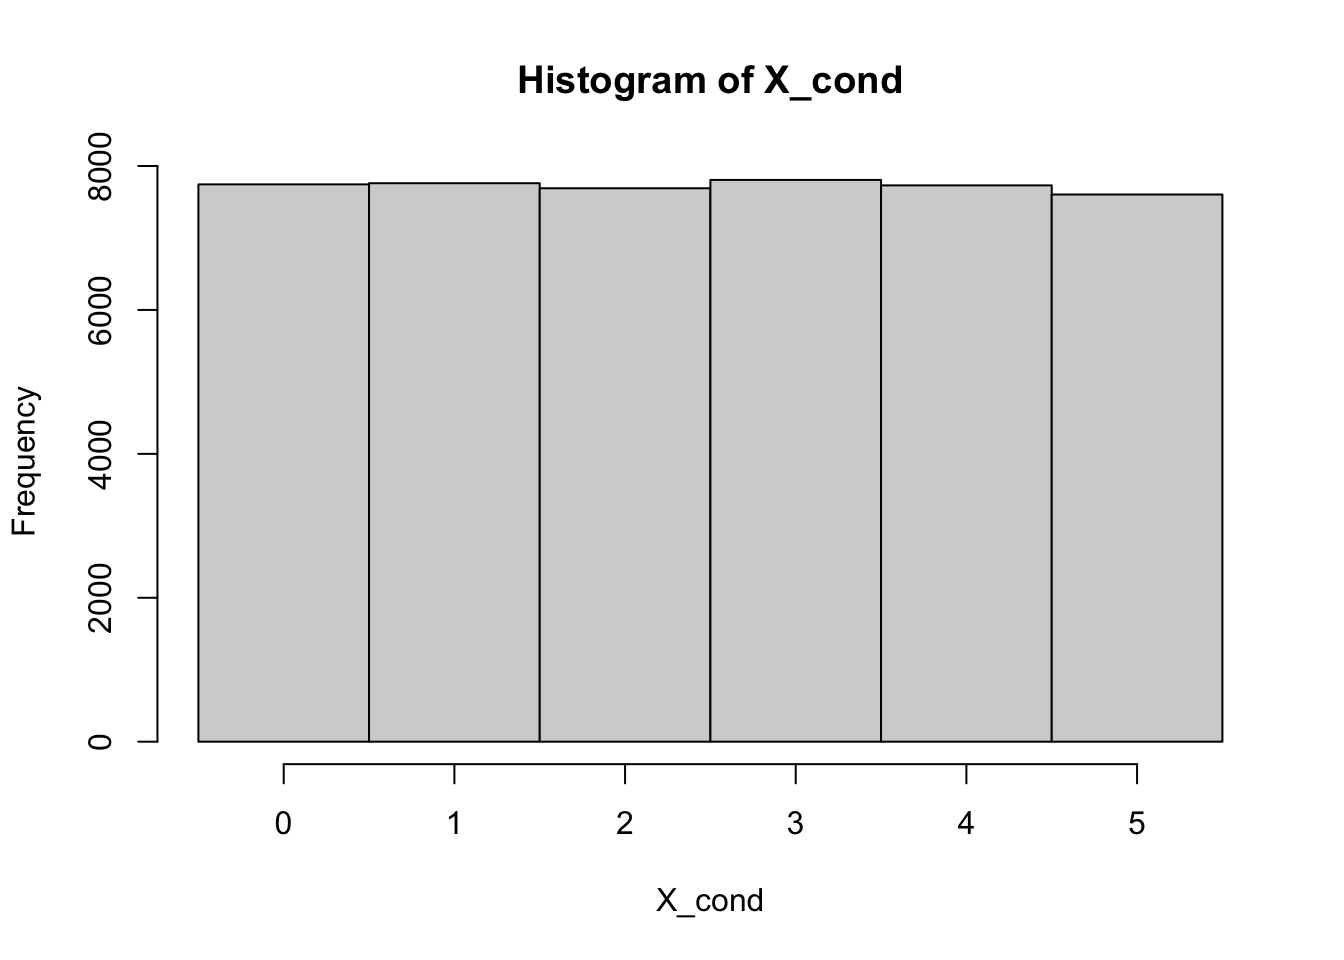
\includegraphics{_main_files/figure-latex/unnamed-chunk-113-1} \end{center}

Since \texttt{X\_cond} contains only discrete values from \(0\) to \(5\), a contingency
table might be a better tool for understanding its distribution:

0

1

2

3

4

5

7745

7761

7691

7807

7731

7604

The histogram and the table above suggest that the distribution of \(X\), given \(Z=5\), is uniform on \(\{0,1,2,3,4,5\}\). It is - a calculation almost identical to the one we performed above gives that \({\mathbb{P}}[ X= i| Z=5] = \frac{1}{6}\) for each \(i=0,1,2,3,4,5\).

One more observation at the end. Note that we drew \(n=1,000,000\) simulations this time. While it is probably an overkill for this particular example, conditional probabilities in general require more simulations than unconditional ones. Of course, that is because we reject most of our original draws. Indeed, the size of the vector \texttt{X\_cond} is 46339 - more than a \(20\)-fold decrease. This fact becomes particularly apparent when we try to use Monte Carlo for conditional distributions associated with \emph{continuous} random vectors as we will see in out next problem.
\end{solution}

\begin{exercise}
Let \(X\) and \(Y\) be independent random variables where \(X\) has the \(N(0,1)\) distribution and \(Y\) the exponential distribution with parameter \(\lambda=1\). Find a graphical approximation to the conditional density of \(Y\), given \(X+Y\geq 1\). Repeat the same, but condition on \(X+Y=1\).
\end{exercise}

\begin{solution}
~

\begin{Shaded}
\begin{Highlighting}[]
\NormalTok{nsim }\OtherTok{=} \FloatTok{1e+05}
\NormalTok{x }\OtherTok{=} \FunctionTok{rnorm}\NormalTok{(nsim)}
\NormalTok{y }\OtherTok{=} \FunctionTok{rexp}\NormalTok{(nsim)}

\NormalTok{cond }\OtherTok{=}\NormalTok{ x }\SpecialCharTok{+}\NormalTok{ y }\SpecialCharTok{\textgreater{}=} \DecValTok{1}
\NormalTok{x\_cond }\OtherTok{=}\NormalTok{ x[cond]}
\FunctionTok{hist}\NormalTok{(x\_cond, }\AttributeTok{breaks =} \DecValTok{100}\NormalTok{)}
\end{Highlighting}
\end{Shaded}

\begin{center}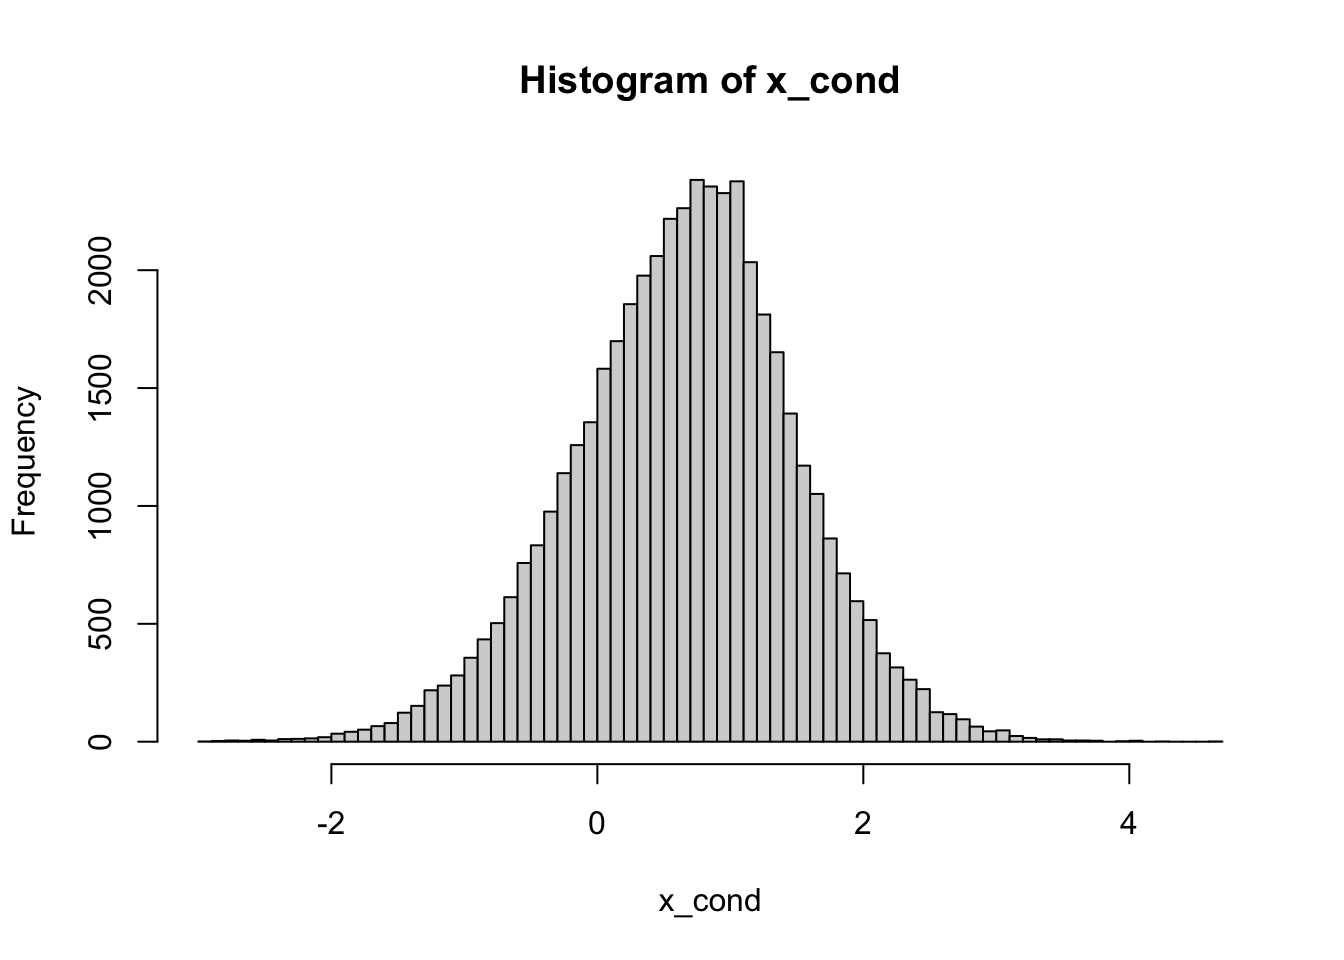
\includegraphics{_main_files/figure-latex/unnamed-chunk-115-1} \end{center}

\begin{Shaded}
\begin{Highlighting}[]
\NormalTok{nsim }\OtherTok{=} \FloatTok{1e+05}
\NormalTok{eps }\OtherTok{=} \FloatTok{0.1}
\NormalTok{x }\OtherTok{=} \FunctionTok{rnorm}\NormalTok{(nsim)}
\NormalTok{y }\OtherTok{=} \FunctionTok{rexp}\NormalTok{(nsim)}
\NormalTok{cond }\OtherTok{=}\NormalTok{ (}\DecValTok{1} \SpecialCharTok{{-}}\NormalTok{ eps }\SpecialCharTok{\textless{}}\NormalTok{ x }\SpecialCharTok{+}\NormalTok{ y) }\SpecialCharTok{\&}\NormalTok{ (x }\SpecialCharTok{+}\NormalTok{ y }\SpecialCharTok{\textless{}} \DecValTok{1} \SpecialCharTok{+}\NormalTok{ eps)}
\NormalTok{x\_cond }\OtherTok{=}\NormalTok{ x[cond]}
\FunctionTok{hist}\NormalTok{(x\_cond, }\AttributeTok{breaks =} \DecValTok{100}\NormalTok{)}
\end{Highlighting}
\end{Shaded}

\begin{center}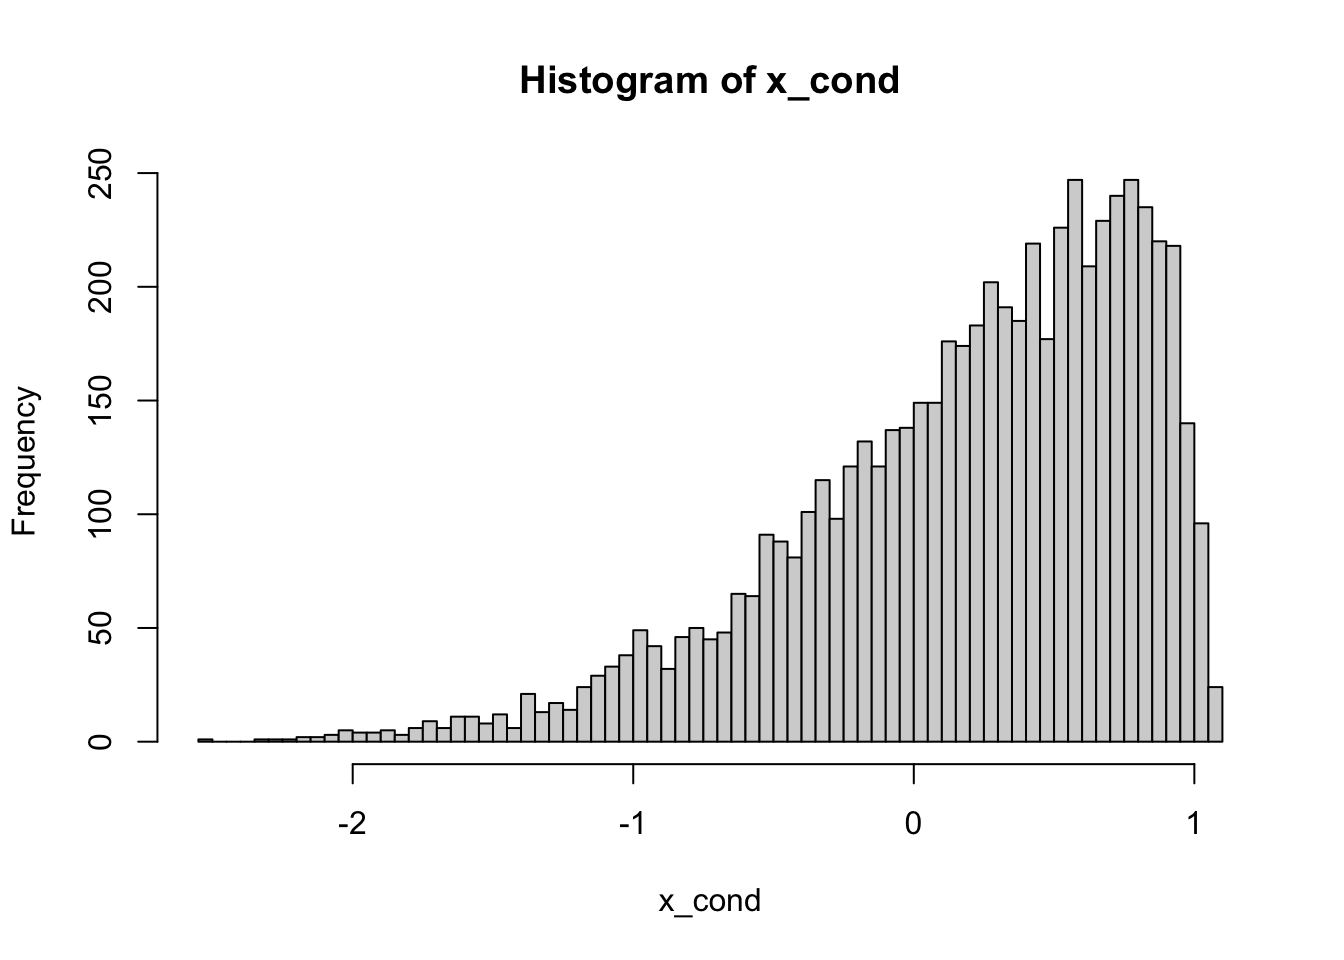
\includegraphics{_main_files/figure-latex/unnamed-chunk-116-1} \end{center}

\emph{Comments (Math):} In the case of conditioning on \(X+Y\geq 1\) we repeated the same procedure as in the discrete case. We simply rejected all draws that do not satisfy the condition.

When Conditioning on \(X+Y=1\), however, you immediately encounter a problem that you don't get with discrete distributions. The event \(\{ X+Y=1\}\) has probability \(0\) and will never happen.
That means that our strategy form the previous problem will simply not work - you will reject \textbf{all} draws. The problem goes beyond a particular approach to the problem, as the conditional probabilities such as \({\mathbb{P}}[ Y \geq 0 | X+Y=1]\) are not well defined. Indeed, the formula
\[ {\mathbb{P}}[ Y \geq 0 | X+Y=1] "=" \frac{{\mathbb{P}}[ Y\geq 0 \text{ and } X+Y=1]}{ {\mathbb{P}}[X+Y=1]}\]
requires that the probability in the denominator be strictly positive. Otherwise you are dividing by zero. The theoretical solution to this is by no means simple and requires mathematics beyond the scope of these notes. Practically, there is a very simple way of going around it. Instead of conditioning on the zero-probability event \(X+Y=1\), we use a slightly more relaxed condition
\[ X+Y \in (1-\varepsilon, 1+\varepsilon) \] for a small, but positive, \(\varepsilon\). In many cases of interest, this approximation works very well, as long as \(\varepsilon\) is not too big. How big? Well, that will depend on the particular problem, as well as on the number of simulations you are drawing. The best way is to try several values and experiment. For example, if we chose \(\varepsilon=0.01\) in our problem, the number of elements in \texttt{x\_cond} (i.e., the number of non-rejected draws) would be on the order of \(100\), which may be considered to small to produce an accurate histogram. On the other hand, when \(\varepsilon=1\), your result will be inaccurate because. The rule of thumb is to take the smallest \(\varepsilon\) you can, while keeping the number of non-rejected draws sufficiently large.
\end{solution}

\hypertarget{additional-problems-for-chapter-2}{%
\section{Additional Problems for Chapter 2}\label{additional-problems-for-chapter-2}}

Click for Solution

Click for Solution

\begin{exercise}
A basic method for obtaining simulations draws from distributions
other than the uniform is the \textbf{transformation method}. The idea is
to start with (pseudo) random numbers, i.e., draws from the uniform
\(U(0,1)\) distribution, and then apply a function \(g\) to each
simulation. The difficulty is, of course, how to choose the right
function \(g\). Let \(X\) be a random variable with a continuous and
strictly increasing cdf \(F\). What is the distribution of \(Y=F (X)\)? What does that have to do with the transformation method?

(Hint: if you are having difficulty with this problem, feel free to
run some experiments using R. )
\end{exercise}

Click for Solution

\begin{solution}
Let us perform an experiment where \(X \sim N(0,1)\). Remembering that the cdf is given by the R function \texttt{pnorm}:

\begin{Shaded}
\begin{Highlighting}[]
\NormalTok{x }\OtherTok{=} \FunctionTok{rnorm}\NormalTok{(}\FloatTok{1e+05}\NormalTok{)}
\NormalTok{y }\OtherTok{=} \FunctionTok{pnorm}\NormalTok{(x)}
\FunctionTok{hist}\NormalTok{(y)}
\end{Highlighting}
\end{Shaded}

\begin{center}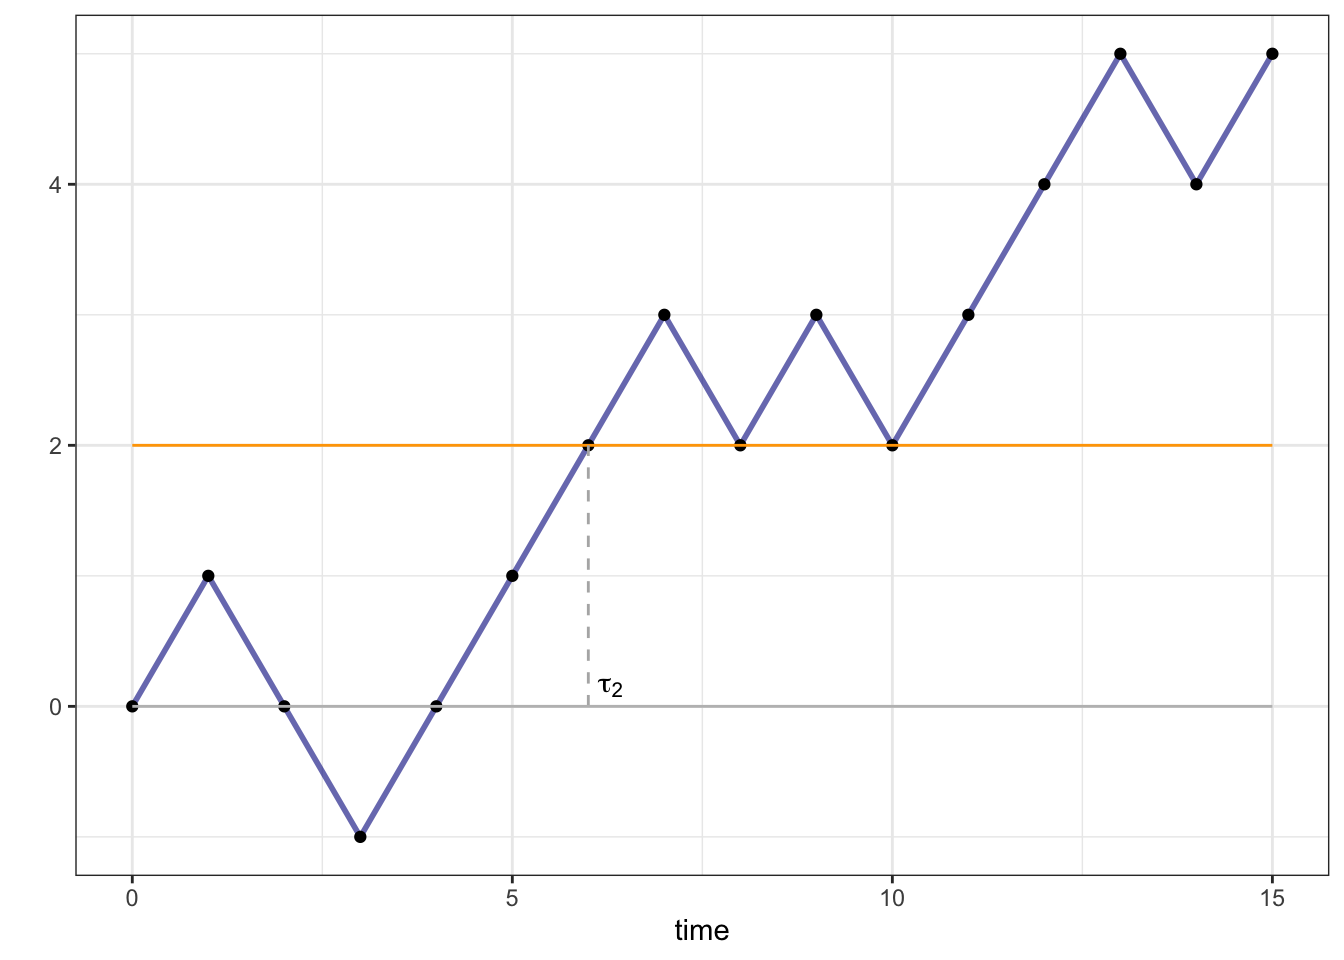
\includegraphics{_main_files/figure-latex/unnamed-chunk-176-1} \end{center}

This looks like a histogram of a uniform distribution on \((0,1)\).
Let's try with some other continuous distributions

\begin{Shaded}
\begin{Highlighting}[]
\NormalTok{x1 }\OtherTok{=} \FunctionTok{rexp}\NormalTok{(}\FloatTok{1e+05}\NormalTok{)}
\NormalTok{x2 }\OtherTok{=} \FunctionTok{rcauchy}\NormalTok{(}\FloatTok{1e+05}\NormalTok{)}
\NormalTok{x3 }\OtherTok{=} \FunctionTok{runif}\NormalTok{(}\FloatTok{1e+05}\NormalTok{)}
\NormalTok{x4 }\OtherTok{=} \FunctionTok{rgamma}\NormalTok{(}\FloatTok{1e+05}\NormalTok{, }\AttributeTok{shape =} \DecValTok{3}\NormalTok{)}
\FunctionTok{par}\NormalTok{(}\AttributeTok{mfrow =} \FunctionTok{c}\NormalTok{(}\DecValTok{2}\NormalTok{, }\DecValTok{2}\NormalTok{))}
\FunctionTok{hist}\NormalTok{(}\FunctionTok{pexp}\NormalTok{(x1))}
\FunctionTok{hist}\NormalTok{(}\FunctionTok{pcauchy}\NormalTok{(x2))}
\FunctionTok{hist}\NormalTok{(}\FunctionTok{punif}\NormalTok{(x3))}
\FunctionTok{hist}\NormalTok{(}\FunctionTok{pgamma}\NormalTok{(x4, }\AttributeTok{shape =} \DecValTok{3}\NormalTok{))}
\end{Highlighting}
\end{Shaded}

\begin{center}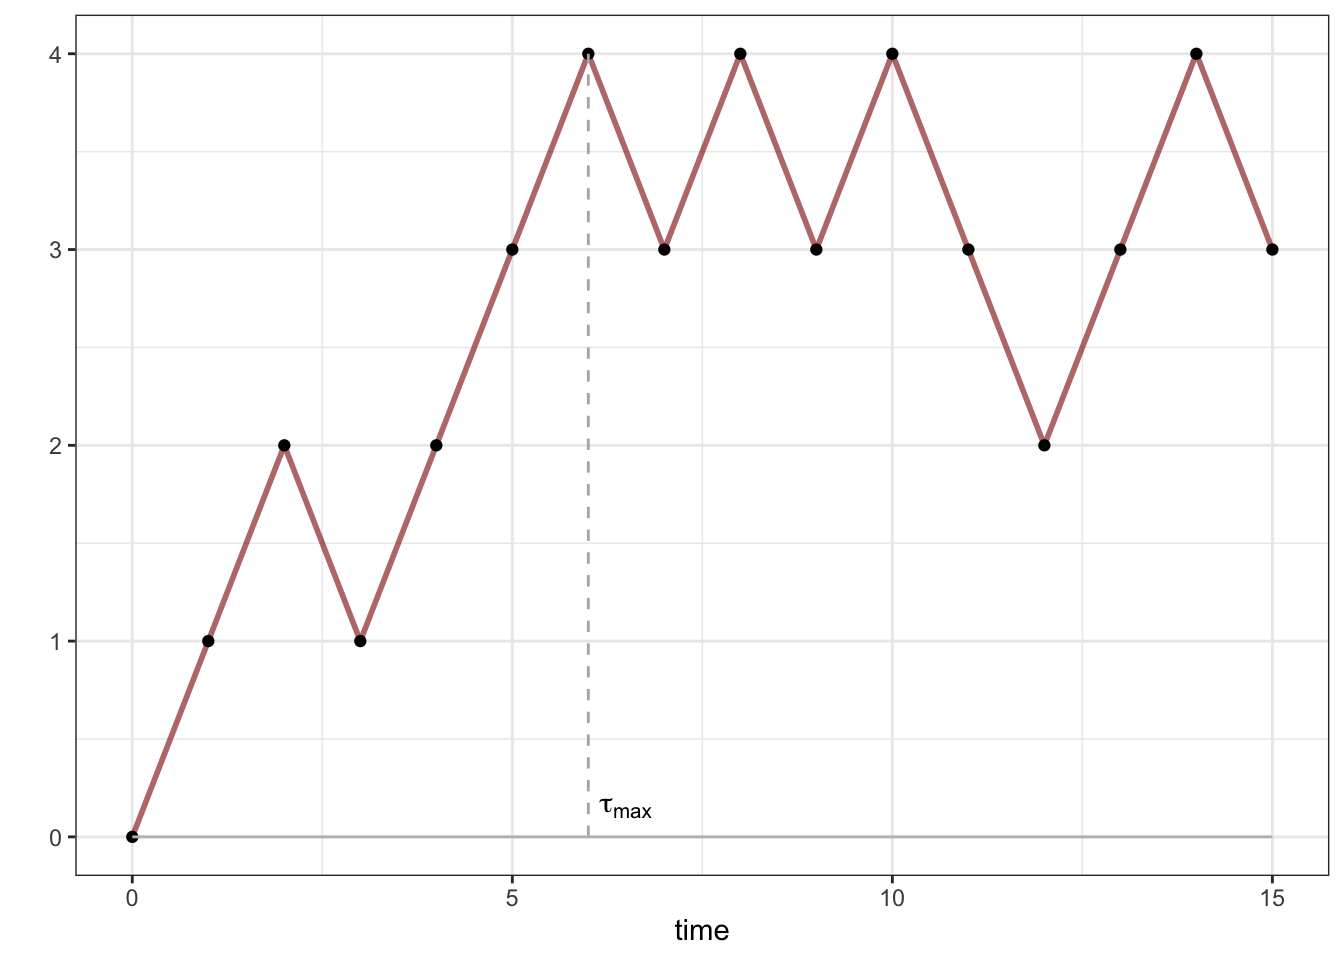
\includegraphics{_main_files/figure-latex/unnamed-chunk-177-1} \end{center}

All of those point to the same conjecture, namely that \(F(X)\) is
uniformly distributed on \((0,1)\).
To prove that, we
take \(Y=F(X)\) and try to compute that cdf \(F_Y\) of \(Y\):
\[F_Y(y) = {\mathbb{P}}[ Y \leq y] = {\mathbb{P}}[ F(X) \leq y]\]
Since \(F\) is strictly increasing, it admits an inverse \(F^{-1}\).
Moreover, for any \(y \in (0,1)\),
the set of all values of \(x\) such that \(F(x)\leq y\) (the red range) is
exactly the interval \((-\infty, F^{-1}(y)]\) (the blue range), as in
the picture below:

\begin{center}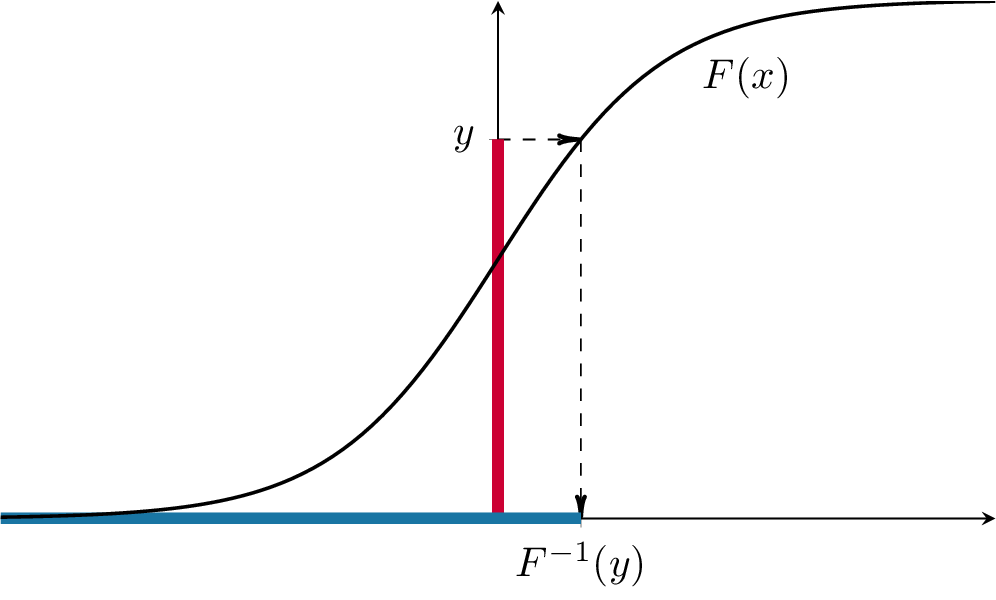
\includegraphics[width=0.6\linewidth,style="padding:10px"]{pics/cdf_plot} \end{center}

Hence, \[F_Y(y)={\mathbb{P}}[Y\leq y] = {\mathbb{P}}[ F(X) \leq y] = {\mathbb{P}}[ X \leq F^{-1}(y) ] = F(F^{-1}(y)) = y, 
\text{ for } y\in (0,1).\] The cdf \(F_Y\) is, therefore, equal to the cdf
of a uniform on \((0,1)\).
Since the cdf uniquely determines the distribution, \(Y\) must be uniformly
distributed on \((0,1)\).
\end{solution}

Click for Solution

\begin{exercise}
Let \texttt{x=rnorm(1000)} and \texttt{y=rnorm(1000)}. For each of the following pairs, use the permutation test to decide whether they are independent or not

\begin{enumerate}
\def\labelenumi{\alph{enumi})}
\tightlist
\item
  \texttt{x\^{}2+y\^{}2} and \texttt{y\^{}2}
\item
  \texttt{(x+y)/sqrt(2)} and \texttt{(x-y)/sqrt(2)}
\item
  \texttt{x} and \texttt{1}
\item
  \texttt{x\^{}2+y\^{}2} and \texttt{atan(y/x)}.
\end{enumerate}

(Note: do not worry about dividing by \(0\) in d.~It will happen with probability \(0\).)
\end{exercise}

Click for Solution

\begin{solution}
Let us start by writing a function to save some keystrokes

\begin{Shaded}
\begin{Highlighting}[]
\NormalTok{permutation\_test }\OtherTok{=} \ControlFlowTok{function}\NormalTok{(z, w) \{}
    \FunctionTok{par}\NormalTok{(}\AttributeTok{mfrow =} \FunctionTok{c}\NormalTok{(}\DecValTok{2}\NormalTok{, }\DecValTok{2}\NormalTok{))}
    \FunctionTok{plot}\NormalTok{(z, w, }\AttributeTok{asp =} \DecValTok{1}\NormalTok{)}
    \FunctionTok{plot}\NormalTok{(z, }\FunctionTok{sample}\NormalTok{(w), }\AttributeTok{asp =} \DecValTok{1}\NormalTok{)}
    \FunctionTok{plot}\NormalTok{(z, }\FunctionTok{sample}\NormalTok{(w), }\AttributeTok{asp =} \DecValTok{1}\NormalTok{)}
    \FunctionTok{plot}\NormalTok{(z, }\FunctionTok{sample}\NormalTok{(w), }\AttributeTok{asp =} \DecValTok{1}\NormalTok{)}
\NormalTok{\}}

\NormalTok{x }\OtherTok{=} \FunctionTok{rnorm}\NormalTok{(}\DecValTok{1000}\NormalTok{)}
\NormalTok{y }\OtherTok{=} \FunctionTok{rnorm}\NormalTok{(}\DecValTok{1000}\NormalTok{)}
\end{Highlighting}
\end{Shaded}

\begin{enumerate}
\def\labelenumi{\alph{enumi})}
\item
\begin{Shaded}
\begin{Highlighting}[]
\FunctionTok{permutation\_test}\NormalTok{(x}\SpecialCharTok{\^{}}\DecValTok{2} \SpecialCharTok{+}\NormalTok{ y}\SpecialCharTok{\^{}}\DecValTok{2}\NormalTok{, y}\SpecialCharTok{\^{}}\DecValTok{2}\NormalTok{)}
\end{Highlighting}
\end{Shaded}

  \begin{center}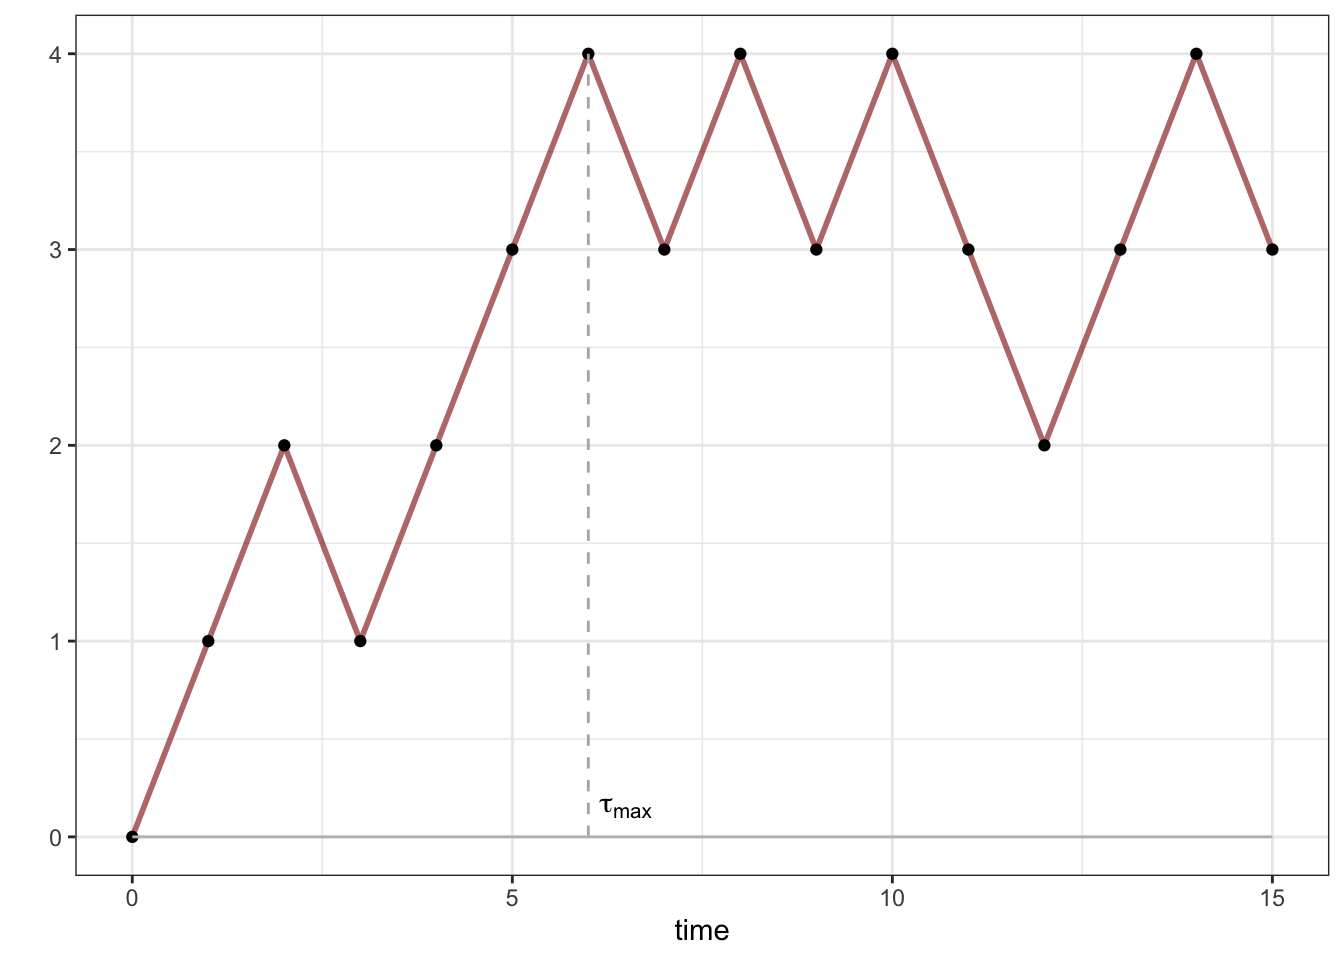
\includegraphics{_main_files/figure-latex/unnamed-chunk-184-1} \end{center}

  The first plot is very different from the other three. Therefore,the vectors are probably \emph{not} independent.
\item
\begin{Shaded}
\begin{Highlighting}[]
\FunctionTok{permutation\_test}\NormalTok{((x }\SpecialCharTok{+}\NormalTok{ y)}\SpecialCharTok{/}\FunctionTok{sqrt}\NormalTok{(}\DecValTok{2}\NormalTok{), (x }\SpecialCharTok{{-}}\NormalTok{ y)}\SpecialCharTok{/}\FunctionTok{sqrt}\NormalTok{(}\DecValTok{2}\NormalTok{))}
\end{Highlighting}
\end{Shaded}

  \begin{center}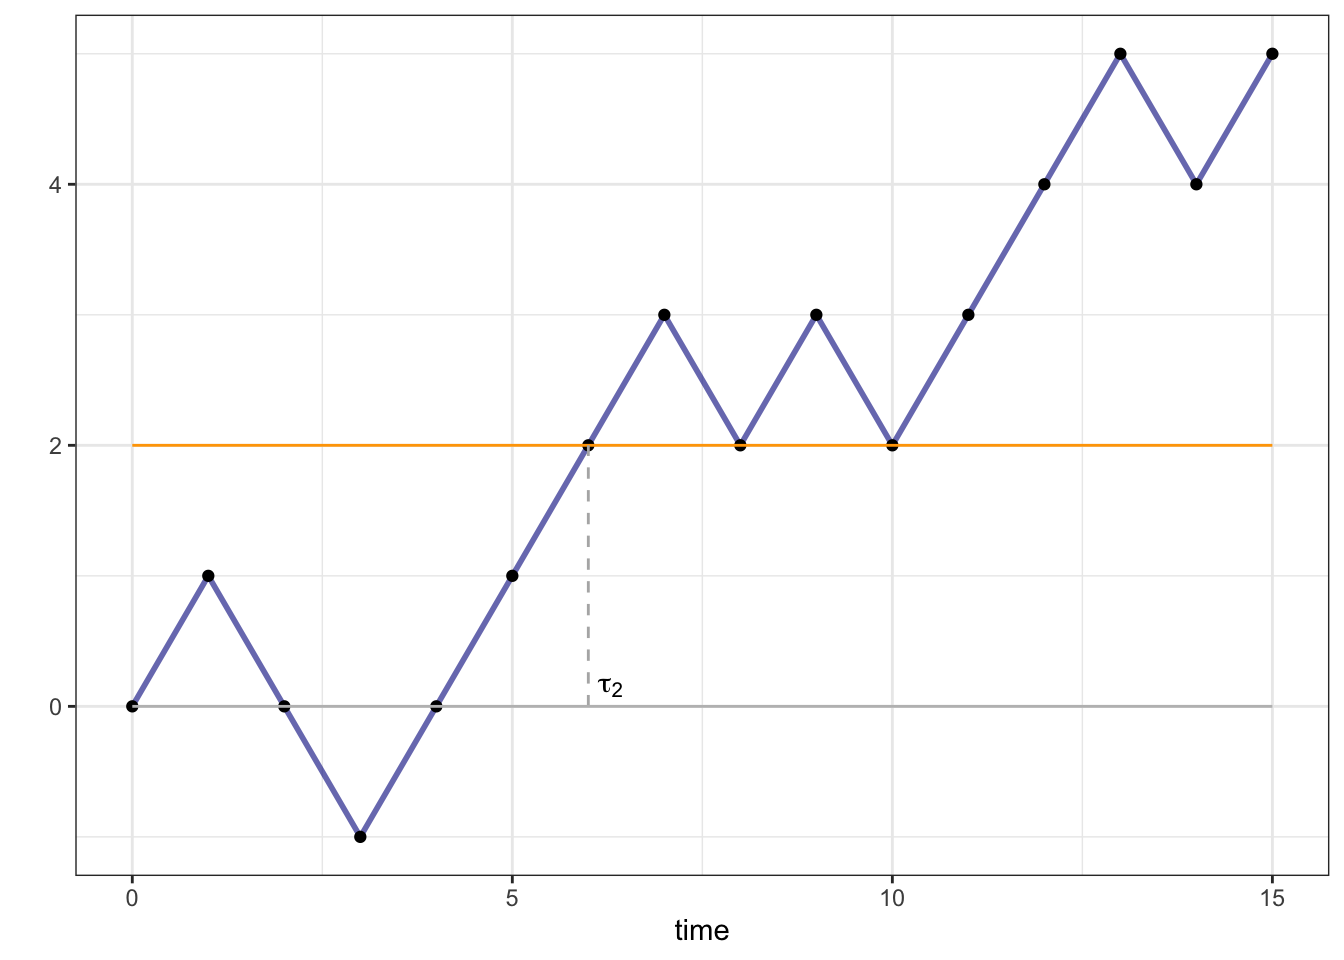
\includegraphics{_main_files/figure-latex/unnamed-chunk-185-1} \end{center}

  The first plot could easily be confused for one of the other three. Therefore the vectors are probably independent.
\item
\begin{Shaded}
\begin{Highlighting}[]
\CommentTok{\# we have to use rep(1,length(x)) to get a vector of 1s of the same length as}
\CommentTok{\# x.  R will not recycle it properly if you simply write 1.  Another, more}
\CommentTok{\# \textquotesingle{}hacky\textquotesingle{} way would be to take advantage of recycling and use 0*x+1}
\FunctionTok{permutation\_test}\NormalTok{(x, }\FunctionTok{rep}\NormalTok{(}\DecValTok{1}\NormalTok{, }\FunctionTok{length}\NormalTok{(x)))}
\end{Highlighting}
\end{Shaded}

  \begin{center}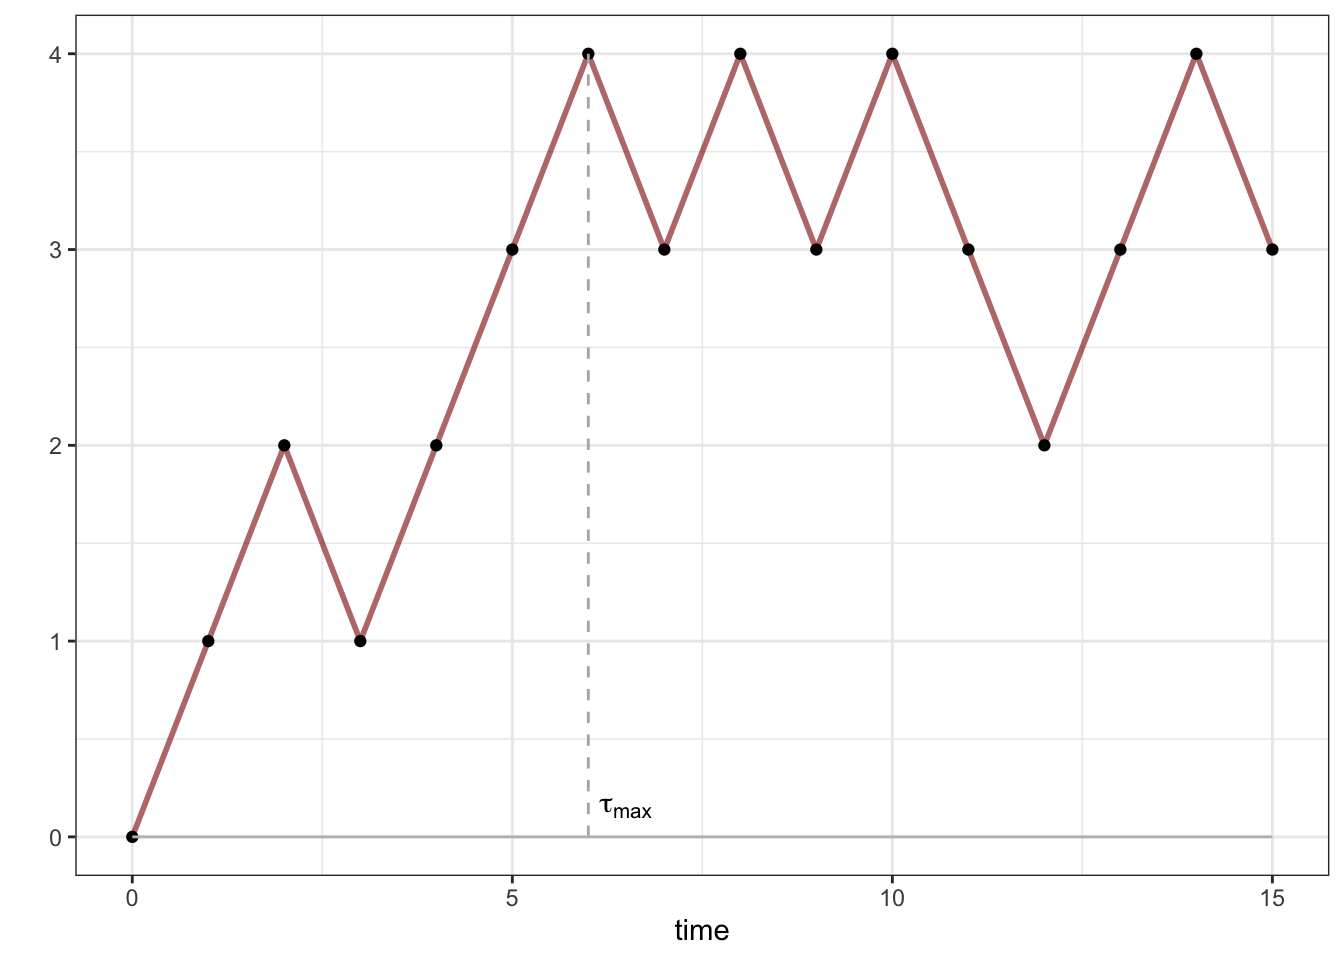
\includegraphics{_main_files/figure-latex/unnamed-chunk-186-1} \end{center}

  The plots look very similar. Therefore, the vectors are probably independent. We could have known this without drawing any graphs. Anything is independent of a constant random variable (vector).
\item
\begin{Shaded}
\begin{Highlighting}[]
\FunctionTok{permutation\_test}\NormalTok{(x}\SpecialCharTok{\^{}}\DecValTok{2} \SpecialCharTok{+}\NormalTok{ y}\SpecialCharTok{\^{}}\DecValTok{2}\NormalTok{, }\FunctionTok{atan}\NormalTok{(y}\SpecialCharTok{/}\NormalTok{x))}
\end{Highlighting}
\end{Shaded}

  \begin{center}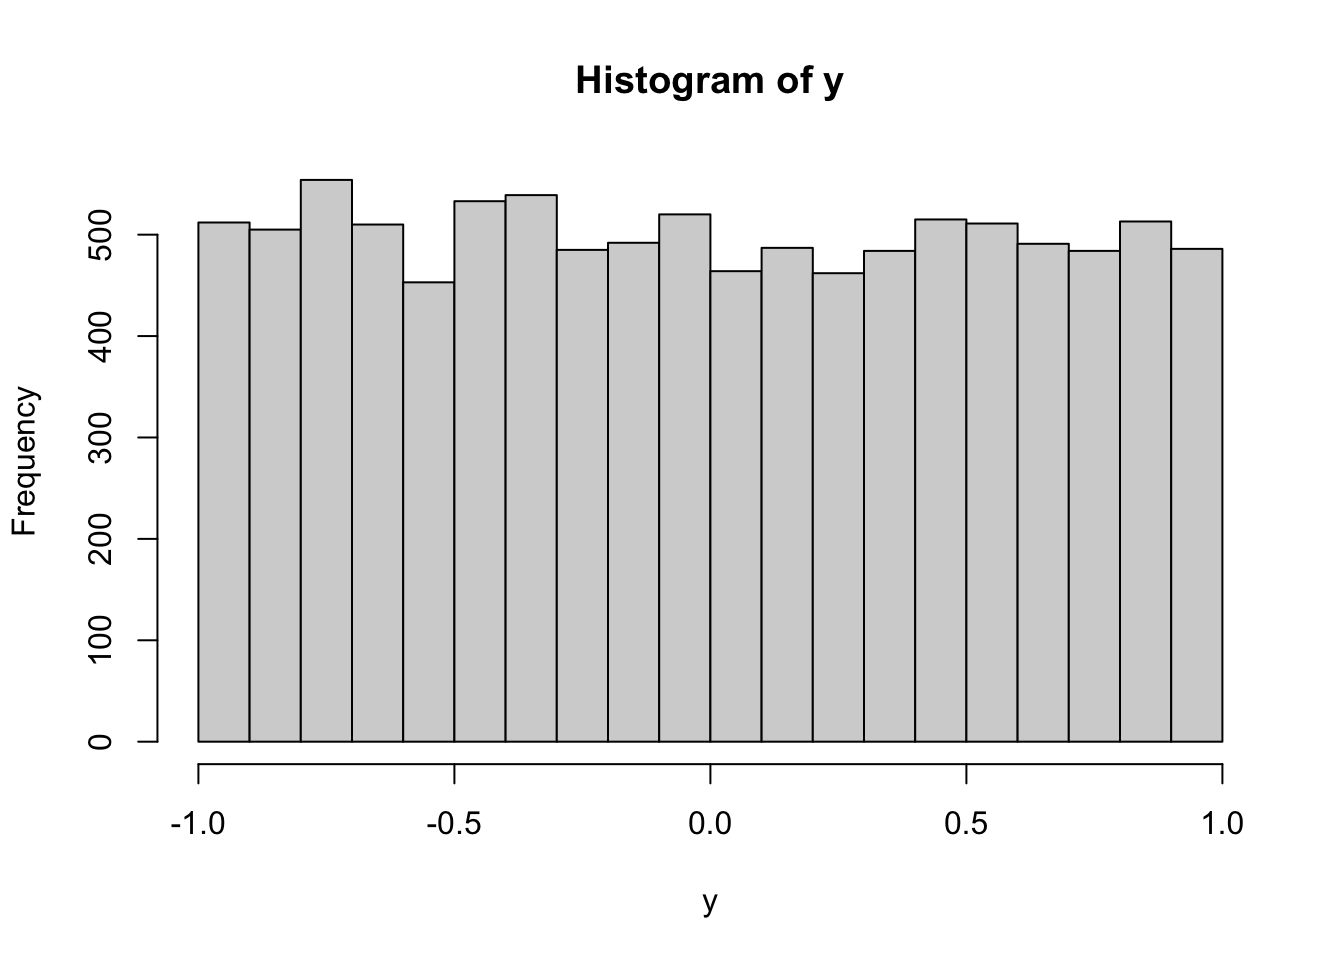
\includegraphics{_main_files/figure-latex/unnamed-chunk-187-1} \end{center}

  Plots look very similar to each other. Therefore, \texttt{z} and \texttt{w} are probably independent.
\end{enumerate}

\emph{Note:} The plots in b) and d) reveal that the distribution of the random vector
\((X,Y)\) consisting of two independent standard normals is probably rotation
invariant. In b) we are asked to compare the coordinates of the vector obtained
from \((X,Y)\) by a rotation at \(45\) degrees around the origin. The fact that
independence persisted suggests that components remain independent even after a
(specific) rotation. If you tried rotations by different angles you would get
the same result. The experiment in d) told us that the (squared) distance
\(X^2+Y^2\) and angle between \((X,Y)\) and the \(x\)-are independent. This is also
something that one would expect from a rotationally-invariant distribution.
Indeed, the distribution of the distance to the origin should not depend on the
direction.

It is important to note that none of this proves anything. It is simply
numerical evidence for a given conclusion.
\end{solution}

\begin{exercise}
Simulate \(n=10000\) draws from the joint distribution given by the following
table:

\begin{table}
\centering
\begin{tabular}{>{}l|r|r|r}
\hline
  & 1 & 2 & 3\\
\hline
\textbf{1} & 0.1 & 0.0 & 0.3\\
\hline
\textbf{2} & 0.1 & 0.1 & 0.0\\
\hline
\textbf{3} & 0.0 & 0.0 & 0.4\\
\hline
\end{tabular}
\end{table}

Display the contingency table of your results, as well as a table
showing the
``errors'', i.e., differences between the theoretical frequencies
(i.e., probabilities given above) and the obtained relative
frequencies in the sample.
\end{exercise}

Click for Solution

Click for Solution

\begin{exercise}
The \textbf{tricylinder} is a solid body constructed as follows: create three
cylinders of radius 1 around each of the three coordinate axes and intersect
them:

Image by Ag2gaeh - Own work, CC BY-SA 4.0, \url{https://commons.wikimedia.org/w/index.php?curid=63604565}

Use Monte Carlo to estimate the volume of the tricylinder and
check your estimate against the exact value \(8(2-\sqrt{2})\).
\end{exercise}

Click for Solution

\begin{solution}
By the very construction, it is clear that the entire tricylinder lies
within the cube \([-1,1]\times [-1,1] \times[-1,1]\). Therefore, we can
compute its volume by simulating random draws from the uniform
distribution in that cube, and computing the relative frequence of
those values that fall inside the tricylinder. The whole point is
that it is easy to check, given a point \((x,y,z)\), whether it lies
inside the tricylinder or not. Indeed, the answer is ``yes'' if and
only if all three of the following inequalities are satisfied: \[
x^2+y^2 \le 1,\  x^2+z^2\leq 1 \text{ and } y^2+z^2\leq 1.\]

\begin{Shaded}
\begin{Highlighting}[]
\NormalTok{nsim }\OtherTok{=} \DecValTok{10000}
\NormalTok{x }\OtherTok{=} \FunctionTok{runif}\NormalTok{(nsim, }\AttributeTok{min =} \SpecialCharTok{{-}}\DecValTok{1}\NormalTok{, }\AttributeTok{max =} \DecValTok{1}\NormalTok{)}
\NormalTok{y }\OtherTok{=} \FunctionTok{runif}\NormalTok{(nsim, }\AttributeTok{min =} \SpecialCharTok{{-}}\DecValTok{1}\NormalTok{, }\AttributeTok{max =} \DecValTok{1}\NormalTok{)}
\NormalTok{z }\OtherTok{=} \FunctionTok{runif}\NormalTok{(nsim, }\AttributeTok{min =} \SpecialCharTok{{-}}\DecValTok{1}\NormalTok{, }\AttributeTok{max =} \DecValTok{1}\NormalTok{)}
\NormalTok{is\_in }\OtherTok{=}\NormalTok{ (x}\SpecialCharTok{\^{}}\DecValTok{2} \SpecialCharTok{+}\NormalTok{ y}\SpecialCharTok{\^{}}\DecValTok{2} \SpecialCharTok{\textless{}=} \DecValTok{1}\NormalTok{) }\SpecialCharTok{\&}\NormalTok{ (x}\SpecialCharTok{\^{}}\DecValTok{2} \SpecialCharTok{+}\NormalTok{ z}\SpecialCharTok{\^{}}\DecValTok{2} \SpecialCharTok{\textless{}=} \DecValTok{1}\NormalTok{) }\SpecialCharTok{\&}\NormalTok{ (y}\SpecialCharTok{\^{}}\DecValTok{2} \SpecialCharTok{+}\NormalTok{ z}\SpecialCharTok{\^{}}\DecValTok{2} \SpecialCharTok{\textless{}=} \DecValTok{1}\NormalTok{)}

\NormalTok{(}\DecValTok{2}\SpecialCharTok{\^{}}\DecValTok{3} \SpecialCharTok{*} \FunctionTok{sum}\NormalTok{(is\_in)}\SpecialCharTok{/}\NormalTok{nsim)}
\DocumentationTok{\#\# [1] 4.708}
\end{Highlighting}
\end{Shaded}

We multiplied by \(2^3\) because that is the volume of the cube
\([-1,1]\times [-1,1] \times [-1,1]\). Without it, we would get the
portion of the cube taken by the tricylinder, and not its volume.

The true value of \(8(2-\sqrt{2})\) is, approximately, \(4.6862\).
\end{solution}

\begin{exercise}[Extra Credit]
Read about the \textbf{Monty Hall Problem} online (the introduction to its
\href{https://en.wikipedia.org/wiki/Monty_Hall_problem}{Wikipedia page} has a nice description),
Use Monte Carlo to compare the two possible strategies (switching and
not-switching) and decide which is better.
\end{exercise}

Click for Solution

\begin{solution}
The host knows where the car is and what contestant's guess is. If those two are the same (i.e., contestant guessed right), he will choose one of the two remaining doors at random. If not, he simply shows the contestant the other door with the goat behind it. This exactly what the function \texttt{show\_door} implements:

\begin{Shaded}
\begin{Highlighting}[]
\NormalTok{show\_door }\OtherTok{=} \ControlFlowTok{function}\NormalTok{(car, guess) \{}
\NormalTok{    all\_doors }\OtherTok{=} \FunctionTok{c}\NormalTok{(}\DecValTok{1}\NormalTok{, }\DecValTok{2}\NormalTok{, }\DecValTok{3}\NormalTok{)}
\NormalTok{    goat\_doors }\OtherTok{=}\NormalTok{ all\_doors[all\_doors }\SpecialCharTok{!=}\NormalTok{ car]}

    \ControlFlowTok{if}\NormalTok{ (car }\SpecialCharTok{==}\NormalTok{ guess) \{}
\NormalTok{        random\_goat\_door }\OtherTok{=} \FunctionTok{sample}\NormalTok{(goat\_doors, }\AttributeTok{size =} \DecValTok{1}\NormalTok{)}
        \FunctionTok{return}\NormalTok{(random\_goat\_door)}
\NormalTok{    \} }\ControlFlowTok{else}\NormalTok{ \{}
\NormalTok{        the\_other\_goat\_door }\OtherTok{=}\NormalTok{ goat\_doors[goat\_doors }\SpecialCharTok{!=}\NormalTok{ guess]}
        \FunctionTok{return}\NormalTok{(the\_other\_goat\_door)}
\NormalTok{    \}}
\NormalTok{\}}
\end{Highlighting}
\end{Shaded}

Next, we write a function which simulates the outcome of a single game. It will have one argument, \texttt{switch} which will determine whether the contestant switches the door or not.

\begin{Shaded}
\begin{Highlighting}[]
\NormalTok{one\_game }\OtherTok{=} \ControlFlowTok{function}\NormalTok{(}\ControlFlowTok{switch}\NormalTok{) \{}
\NormalTok{    all\_doors }\OtherTok{=} \FunctionTok{c}\NormalTok{(}\DecValTok{1}\NormalTok{, }\DecValTok{2}\NormalTok{, }\DecValTok{3}\NormalTok{)}
\NormalTok{    car }\OtherTok{=} \FunctionTok{sample}\NormalTok{(all\_doors, }\AttributeTok{size =} \DecValTok{1}\NormalTok{)}
\NormalTok{    guess }\OtherTok{=} \FunctionTok{sample}\NormalTok{(all\_doors, }\AttributeTok{size =} \DecValTok{1}\NormalTok{)}

    \ControlFlowTok{if}\NormalTok{ (}\ControlFlowTok{switch}\NormalTok{) \{}
\NormalTok{        unguessed\_doors }\OtherTok{=}\NormalTok{ all\_doors[all\_doors }\SpecialCharTok{!=}\NormalTok{ guess]}
\NormalTok{        shown\_door }\OtherTok{=} \FunctionTok{show\_door}\NormalTok{(car, guess)}
\NormalTok{        switched\_guess }\OtherTok{=}\NormalTok{ unguessed\_doors[unguessed\_doors }\SpecialCharTok{!=}\NormalTok{ shown\_door]}
        \FunctionTok{return}\NormalTok{(switched\_guess }\SpecialCharTok{==}\NormalTok{ car)}
\NormalTok{    \} }\ControlFlowTok{else}\NormalTok{ \{}
        \FunctionTok{return}\NormalTok{(guess }\SpecialCharTok{==}\NormalTok{ car)}
\NormalTok{    \}}
\NormalTok{\}}
\end{Highlighting}
\end{Shaded}

Finally we run two batches of \(10,000\) simulations, one with \texttt{switch=TRUE} and another with \texttt{switch=FALSE}:

\begin{Shaded}
\begin{Highlighting}[]
\NormalTok{nsim }\OtherTok{=} \DecValTok{10000}
\NormalTok{switch\_doors }\OtherTok{=} \FunctionTok{replicate}\NormalTok{(nsim, }\FunctionTok{one\_game}\NormalTok{(}\ConstantTok{TRUE}\NormalTok{))}
\NormalTok{dont\_switch\_doors }\OtherTok{=} \FunctionTok{replicate}\NormalTok{(nsim, }\FunctionTok{one\_game}\NormalTok{(}\ConstantTok{FALSE}\NormalTok{))}
\NormalTok{(}\AttributeTok{prob\_with\_switching =} \FunctionTok{mean}\NormalTok{(switch\_doors))}
\DocumentationTok{\#\# [1] 0.668}
\NormalTok{(}\AttributeTok{prob\_without\_switching =} \FunctionTok{mean}\NormalTok{(dont\_switch\_doors))}
\DocumentationTok{\#\# [1] 0.3288}
\end{Highlighting}
\end{Shaded}

Therefore, the probability of winning after switching is about double the probability of winning without switching. Switching is good for you!

(A philosophical note: this was the most ``agnostic'' approach to this simulation. Simulations can often be simplified with a bit of insight. For example, we could have realized that the switching strategy simply flips the correctness of the guess (from ``correct'' to ``wrong'' and vice versa) and used it to write a much shorter answer. Ultimately, we could have realized that, because the probability of the initial guess being correct is \(1/3\), switching leads to a correct guess in \(2/3\) of the cases (and not switching in only \(1/3\) of the cases). In this case, the whole code would be \texttt{sample(c("correct",\ "incorrect"),\ size=10000,\ prob=\ c(2/3,1/3),\ replacement=TRUE)}, which is an extremely inefficient way to estimate the value of the number \(2/3\)!)
\end{solution}

Click for Solution

Click for Solution

\begin{exercise}
We learned how to simulate from a joint distribution of two discrete vectors
\((X,Y\)) by thinking of it as one-dimensional distribution but with values
represented by pairs of numbers. Here is another way this can be done:

\begin{enumerate}
\def\labelenumi{\alph{enumi}.}
\item
  Find the marginal distribution of one of them, say \(X\), and simulate from it
\item
  Given the value you just obtained, let's call it \(x\), simulate from the conditional distribution of \(Y\), given \(X=x\).
\end{enumerate}

Implement this procedure on the following joint distribution:

\begin{table}
\centering
\begin{tabular}{>{}l|r|r|r}
\hline
  & 1 & 2 & 3\\
\hline
\textbf{1} & 0.1 & 0.0 & 0.3\\
\hline
\textbf{2} & 0.1 & 0.1 & 0.0\\
\hline
\textbf{3} & 0.0 & 0.0 & 0.4\\
\hline
\end{tabular}
\end{table}

Display the contingency table of your simulations, first using counts, and then
using relative frequencies. Compare to the theoretical values (i.e., the
probabilities in the table above).
\end{exercise}

Click for Solution

\begin{solution}
~

\begin{Shaded}
\begin{Highlighting}[]
\NormalTok{margin\_X }\OtherTok{=} \FunctionTok{c}\NormalTok{(}\FloatTok{0.2}\NormalTok{, }\FloatTok{0.1}\NormalTok{, }\FloatTok{0.7}\NormalTok{ )}
\NormalTok{cond\_Y\_X }\OtherTok{=} \FunctionTok{matrix}\NormalTok{(}
   \FunctionTok{c}\NormalTok{( }\FloatTok{0.5}\NormalTok{, }\FloatTok{0.0}\NormalTok{, }\DecValTok{3}\SpecialCharTok{/}\DecValTok{7}\NormalTok{,}
      \FloatTok{0.5}\NormalTok{, }\FloatTok{1.0}\NormalTok{, }\FloatTok{0.0}\NormalTok{,}
      \FloatTok{0.0}\NormalTok{, }\FloatTok{0.0}\NormalTok{, }\DecValTok{4}\SpecialCharTok{/}\DecValTok{7}\NormalTok{),}
   \AttributeTok{byrow=}\ConstantTok{TRUE}\NormalTok{,}
   \AttributeTok{nrow=}\DecValTok{3}\NormalTok{)}

\NormalTok{single\_draw }\OtherTok{=} \ControlFlowTok{function}\NormalTok{() \{}
\NormalTok{   x }\OtherTok{=} \FunctionTok{sample}\NormalTok{(}\FunctionTok{c}\NormalTok{(}\DecValTok{1}\NormalTok{,}\DecValTok{2}\NormalTok{,}\DecValTok{3}\NormalTok{), }\AttributeTok{size=}\DecValTok{1}\NormalTok{, }\AttributeTok{prob=}\NormalTok{margin\_X)}
\NormalTok{   y }\OtherTok{=} \FunctionTok{sample}\NormalTok{(}\FunctionTok{c}\NormalTok{(}\DecValTok{1}\NormalTok{,}\DecValTok{2}\NormalTok{,}\DecValTok{3}\NormalTok{), }\AttributeTok{size=}\DecValTok{1}\NormalTok{, }\AttributeTok{prob=}\NormalTok{cond\_Y\_X[,x])}
   \FunctionTok{return}\NormalTok{(}\FunctionTok{c}\NormalTok{(x,y))}
\NormalTok{\}}

\NormalTok{nsim}\OtherTok{=}\DecValTok{10000}
\NormalTok{df }\OtherTok{=} \FunctionTok{data.frame}\NormalTok{(}
   \FunctionTok{t}\NormalTok{(}\FunctionTok{replicate}\NormalTok{(nsim, }\FunctionTok{single\_draw}\NormalTok{()))}
\NormalTok{)}
\FunctionTok{colnames}\NormalTok{(df) }\OtherTok{=} \FunctionTok{c}\NormalTok{(}\StringTok{"x"}\NormalTok{,}\StringTok{"y"}\NormalTok{)}
\FunctionTok{t}\NormalTok{(}\FunctionTok{table}\NormalTok{(df))}
\DocumentationTok{\#\#    x}
\DocumentationTok{\#\# y      1    2    3}
\DocumentationTok{\#\#   1  962    0 2963}
\DocumentationTok{\#\#   2 1012 1023    0}
\DocumentationTok{\#\#   3    0    0 4040}
\end{Highlighting}
\end{Shaded}

The variables \texttt{margin\_X} and \texttt{cond\_X\_Y} are what you get when you compute the marginal and the conditional distribution from the given joint-distribution table as you did in your probability class.

The function \texttt{single\_draw} performs a single draw form the distribution of \((X,Y)\) by first drawing the value of \(X\) from its marginal distribution. Then, it chooses the row of the conditional distribution table according to the obtained value of \(X\) and simulates from it.

The function \texttt{replicate} is used to repeat \texttt{single\_draw} many times and collect the results. By default, \texttt{replicate} attaches the output of each new ``replication'' as a new column and not a row, so we need to transpose the final product. That is what the function \texttt{t()} is for. We turn the result into a data frame because the function \texttt{table} knows how to handle data frames automatically. Another use of the transpose gives \texttt{x} the horizontal axis, and \texttt{y} the vertical one, like in the statement of the problem.
\end{solution}

Click for Solution

Click for Solution

\begin{exercise}
Exactly one percent of the people in a given population have a certain
disease. The accuracy of the diagnostic test for it is such that it
detects the sick as sick with probability \(0.95\) and the healthy as
healthy with probability \(0.9\). A person chosen at random from the
population tested positive. What is the probability the he/she is, in
fact, sick. Do the problem both analytically and by Monte Carlo.
\end{exercise}

Click for Solution

\begin{exercise}
A point is chosen at random, uniformly in the unit cube \([0,1]\times [0,1]\times [0,1]\). Its distance to the origin \((0,0)\) is measured,
and turns out to be equal to \(1.5\).

Use simulations to estimate the shape of the pdf of the conditional
distribution of the point's distance to \((1,1,1)\). Compare
it to the unconditional case, i.e., the case where no information
about the distance to \((0,0,0)\) is known.

Compute the mean of this (conditional) distribution for a few values
of the parameter \(\varepsilon\) you use to deal with conditioning in the
continuous case. Make sure you include values of \(\varepsilon\) on both sides
of the spectrum - too big, and too small.
\end{exercise}

Click for Solution

Click for Solution

\hypertarget{endnotes-1}{%
\section{Endnotes}\label{endnotes-1}}

\hypertarget{appendix-appendix}{%
\appendix}


\hypertarget{dist}{%
\chapter{Probability Distributions}\label{dist}}

Here are the basic facts about the probability distributions we will need in these lecture notes. For a much longer list of important distributions, check this \href{https://en.wikipedia.org/wiki/List_of_probability_distributions}{wikipedia page}.

\hypertarget{discrete-distributions}{%
\section{Discrete distributions:}\label{discrete-distributions}}

Note: \((q=1-p)\)

\begin{tabular}{>{}l|l|l|l|l|l|l}
\hline
 & Parameters & Notation & Support & pmf & \$\textbackslash{}EE[X]\$ & \$\textbackslash{}Var[X]\$\\
\hline
\em{\textbf{Bernoulli}} & \em{\$p\textbackslash{}in (0,1)\$} & \em{\$B(p)\$} & \em{\$\textbackslash{}\{0,1\textbackslash{}\}\$} & \em{\$(q,p,0,0,\textbackslash{}dots)\$} & \em{\$p\$} & \em{\$pq\$}\\
\hline
\textbf{Binomial} & \$n\textbackslash{}in\textbackslash{}N , p\textbackslash{}in (0,1)\$ & \$b(n,p)\$ & \$\textbackslash{}\{0,1,\textbackslash{}dots, n\textbackslash{}\}\$ & \$\textbackslash{}binom\{n\}\{k\} p\textasciicircum{}k q\textasciicircum{}\{n-k\}\$ & \$np\$ & \$npq\$\\
\hline
\textbf{Geometric} & \$p\textbackslash{}in (0,1)\$ & \$g(p)\$ & \$\textbackslash{}\{0,1,\textbackslash{}dots\textbackslash{}\}\$ & \$p q\textasciicircum{}k\$ & \$q/p\$ & \$q/p\textasciicircum{}2\$\\
\hline
\textbf{Poisson} & \$\textbackslash{}lambda\textbackslash{}in(0,\textbackslash{}infty)\$ & \$P(\textbackslash{}lambda)\$ & \$\textbackslash{}\{0,1,\textbackslash{}dots\textbackslash{}\}\$ & \$e\textasciicircum{}\{-\textbackslash{}lambda\} \textbackslash{}tfrac\{\textbackslash{}lambda\textasciicircum{}k\}\{k!\}\$ & \$\textbackslash{}lambda\$ & \$\textbackslash{}lambda\$\\
\hline
\end{tabular}

\hypertarget{continuous-distributions}{%
\section{Continuous distributions:}\label{continuous-distributions}}

Note: the pdf is given by the formula in the table only on its support. It is equal to \(0\) outside of it.

\begin{tabular}{>{}l|l|l|l|l|l|l}
\hline
 & Parameters & Notation & Support & pdf & \$\textbackslash{}EE[X]\$ & \$\textbackslash{}Var[X]\$\\
\hline
\em{\textbf{Uniform}} & \em{\$a\textbackslash{}lt b\$} & \em{\$U(a,b)\$} & \em{\$(a,b)\$} & \em{\$\textbackslash{}frac\{1\}\{b-a\}\$} & \em{\$\textbackslash{}frac\{a+b\}\{2\}\$} & \em{\$\textbackslash{}frac\{(b-a)\textasciicircum{}2\}\{12\}\$}\\
\hline
\textbf{Normal} & \$\textbackslash{}mu\textbackslash{}in\{\textbackslash{}mathbb R\},\textbackslash{}sigma \textbackslash{}gt 0\$ & \$N(\textbackslash{}mu,\textbackslash{}sigma)\$ & \$\{\textbackslash{}mathbb R\}\$ & \$\textbackslash{}frac\{1\}\{\textbackslash{}sigma \textbackslash{}sqrt\{2\textbackslash{}pi\}\} e\textasciicircum{}\{-\textbackslash{}tfrac\{(x-\textbackslash{}mu)\textasciicircum{}2\}\{2 \textbackslash{}sigma\textasciicircum{}2\}\}\$ & \$\textbackslash{}mu\$ & \$\textbackslash{}sigma\textasciicircum{}2\$\\
\hline
\textbf{Exponential} & \$\textbackslash{}lambda\textbackslash{}gt 0\$ & \$\textbackslash{}operatorname\{Exp\}(\textbackslash{}lambda)\$ & \$(0,\textbackslash{}infty)\$ & \$\textbackslash{}lambda e\textasciicircum{}\{-\textbackslash{}lambda x\}\$ & \$\textbackslash{}tfrac\{1\}\{\textbackslash{}lambda\}\$ & \$\textbackslash{}frac\{1\}\{\textbackslash{}lambda\textasciicircum{}2\}\$\\
\hline
\end{tabular}

\end{document}
